\documentclass[compress,11pt]{beamer}

%%% Unknown packages
%\usepackage{beamerthemesplit}
%\usepackage{times}

% Provides script capital letters for math
\usepackage{mathrsfs}
\usepackage{diss}
\usepackage{movie15}
\usepackage{subfigure}

%%% Fonts. Default font is computer modern
%\usefonttheme{default}
%\usefonttheme{professionalfonts} %allows you to use an external font w/o beamer replacements


\usefonttheme{serif}

%% \usefonttheme[
%%   %onlysmall,
%%   onlylarge
%%   ] {structureitalicserif} %typesets structural text in italics with serifs

%% \usefonttheme[
%%   %onlysmall,
%%   onlylarge
%%   ] {structuresmallcapsserif} %Doesn't look too bad with onlylarge set

%%  \usefonttheme[
%%    % stillsansserifmath,
%%    % stillsansserifsmall,
%%    % stillsansseriftext,
%%    onlymath
%%  ]{serif} %onlymath option doesn't look too bad, eqns are more readable this way.


%%% Font families
%\usepackage{mathptmx} % not avail?
%\usepackage{helvet} % Helvetica is the standard sansserif font if you do not use the serif theme
%\usepackage{avant}   % fat, bubble-like sans serif letters
%\usepackage{chancery} % not available?
%\usepackage{utopia}  % not available?
%\usepackage{charter} % n/a
%\usepackage{times}

% A computer modern font available in T1 encoding.  As far as I
% can tell it doesn't look much different.
%\usepackage{lmodern}
%\usepackage[T1]{fontenc}



%%% Control the position of progress bars, titles, subtitles, etc. 
%\usetheme{default} % No navigation bars!
%\usetheme{boxes} % puts a box a in the head and footline, looks like default unless
                 % you also use \addheadbox and \addfootbox
%\usetheme{Bergen} % huge left-hand column. informal feel
%\usetheme{Boadilla} % shows page count at bottom.  requires institute
%\usetheme{Madrid} % Like Boadilla, but more color contrast
%\usetheme{Pittsburgh} % right-flushed titles, otherwise very sparse
%\usetheme{Rochester}  % Huge title bars dominating the slide. square corners, no drop shadows
%\usetheme{Antibes}     % Large, Tree-based navigation at the top with sharp corners. Not bad
%\usetheme{JuanLesPins}  % Smooth version of Antibes, no lines in nav tree.
%\usetheme{Montpellier}  % To me, it looks like Antibes.  No box backgrounds.
%\usetheme{Darmstadt} %fuzzy top title bars, drop shadows, circle bullets,
                     % no side column. The top title is very busy
%\usetheme{Frankfurt}  % fuzzy title bars running across
                      % the top only, circular bullets, drop shadows,
                      % colored blocks with rounded corners, pretty nice
%\usetheme{Warsaw}  % Centrally divided top menu, no progress bullets, top
                   % of the screen is a bit busy but otherwise nice
%\usetheme{Berlin} % Square edges and bullets, no drop shadows, no rounded blocks
%\usetheme{Ilmenau} % Similar to Berlin, mini-nav frame, no drop shadows, rounded corners
%\usetheme{Dresden} % Like Berlin, but no block outlines. minimal context, lots of nav, but not bad
\usetheme{Darmstadt} % Berlin with no bottom nav and rounded blocks, pretty nice, a bit too much at top though
%\usetheme{Frankfurt} % Very nice! Like Darmstadt but with less nav at the top
%\usetheme{Singapore} % top title bar has a faded appearance, centered title names, minimal bullets.
%\usetheme{Szeged} % Lots of horizontal lines. Pretty nice but too cluttered at the top

% \usetheme{Berkeley} %side-bar menu screws up the spacing of slides somewhat, use with sidebartab
% \usecolortheme{sidebartab} % You really can't have long section names for this one

%\usetheme{Copenhagen} % tabular navigation, flat look (no shadows) too much top clutter
%\usetheme{Malmoe} % top cluttered
%\usetheme{Luebeck} % top cluttered
%\usetheme{Warsaw} % top is cluttered and even has a drop shadow


% \usetheme{Goettingen} % Looks like Berkely, but less obtrusive nav bar is on the right
% \usecolortheme{sidebartab} % Used with sidebartab, it's really not bad

%\usetheme{Marburg} % A more dominant Goettingen, harder to read sidebar

%\usetheme{Hannover} % right flush titles, left-side nav, top looks a little empty

%\usecolortheme{sidebartab}

%%% Color Themes: Make your colors bolder or more muted
%\usecolortheme{seahorse} % outer color theme, muted grey, a really nice one!, use with rose
                          % or lilly inner color themes
%\usecolortheme{rose}      % dark blue with relatively stark constrast levels
%\usecolortheme{lily}       % as above, but blocks do not have backround color
\usepackage{times}
\usepackage{units}


%\usecolortheme{rose}
%\usecolortheme{seahorse}
\usecolortheme{dolphin}

\setbeamercovered{transparent}
\logo{
\includegraphics[width=.5in]{figures/nasalogo}}
%\logo{
\includegraphics[width=.5in]{figures/meatball}}
%\setbeamercolor{title}{fg=red!80!black,bg=red!20!white}

\title{SUPG Finite Element Simulations of Compressible Flows for Aerothermodynamic Applications}
\author{Benjamin S. Kirk \\ \texttt{\scriptsize benjamin.kirk@nasa.gov}}
\institute[NASA JSC]{Applied Aeroscience \& CFD Branch \\ Aerosciences \& Flight Mechanics Division \\ NASA Lyndon B. Johnson Space Center}
%\date{\today}
\date{February 23, 2007}

\setcounter{tocdepth}{2}
%\AtBeginSection[]{\frame{\tableofcontents[current]}}

\begin{document}

\setbeamertemplate{navigation symbols}{}
  
\frame{\titlepage}

\section[Outline]{}
\frame
{
  \scriptsize
  \tableofcontents
}


\section{Introduction}
\subsection{Background}
\frame
 {
   \vspace{-2em}
   The physical phenomenon of interest is high-speed gas dynamics
   \footnotesize
   \begin{columns}[t]
     %\pause
     \column{.5\textwidth}
     \begin{block}{Physics}
       \begin{itemize}
         \item The compressible Navier-Stokes equations describe fluid flow for \emph{all} Mach numbers
	 \item For aerospace applications of interest the Reynolds number is almost always such that the flows are \emph{convection dominated}
	 \item Multiscale phenomena in the form of shock waves, boundary layers, and shear layers
       \end{itemize}
     \end{block}
     %\pause
     \column{.5\textwidth}
     \begin{block}{Numerics}
       \begin{itemize}
         \item Discretization of the \emph{conservation law form} of the Navier-Stokes equations is required for convergence to physically valid solutions
	 \item Convective terms must be treated with some form of \emph{upwinding}
	 \item Shocks are treated with some form of \emph{limiting} or \emph{shock capturing}, both of which amount to artificial diffusion which regularizes the problem
       \end{itemize}
     \end{block}
   \end{columns}
   \normalsize
 }
 
\frame
{
  \frametitle{Aerodynamics}
  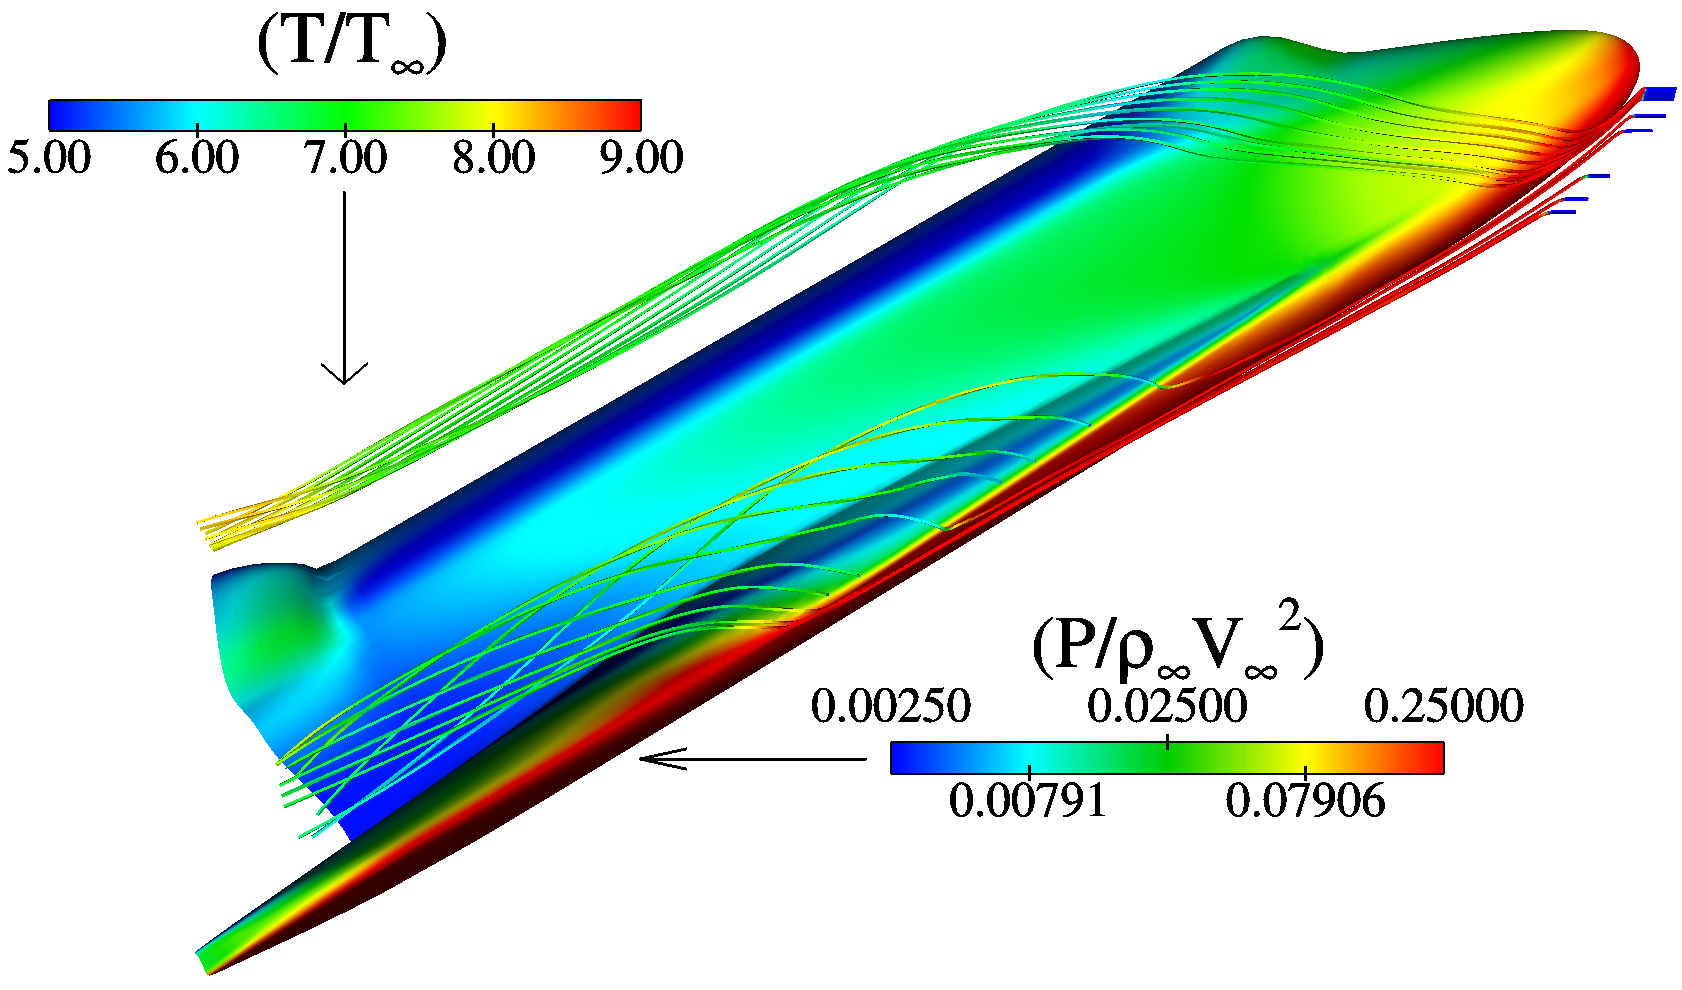
\includegraphics[width=.33\textwidth]{figures/orbiter/side_view_a30}
  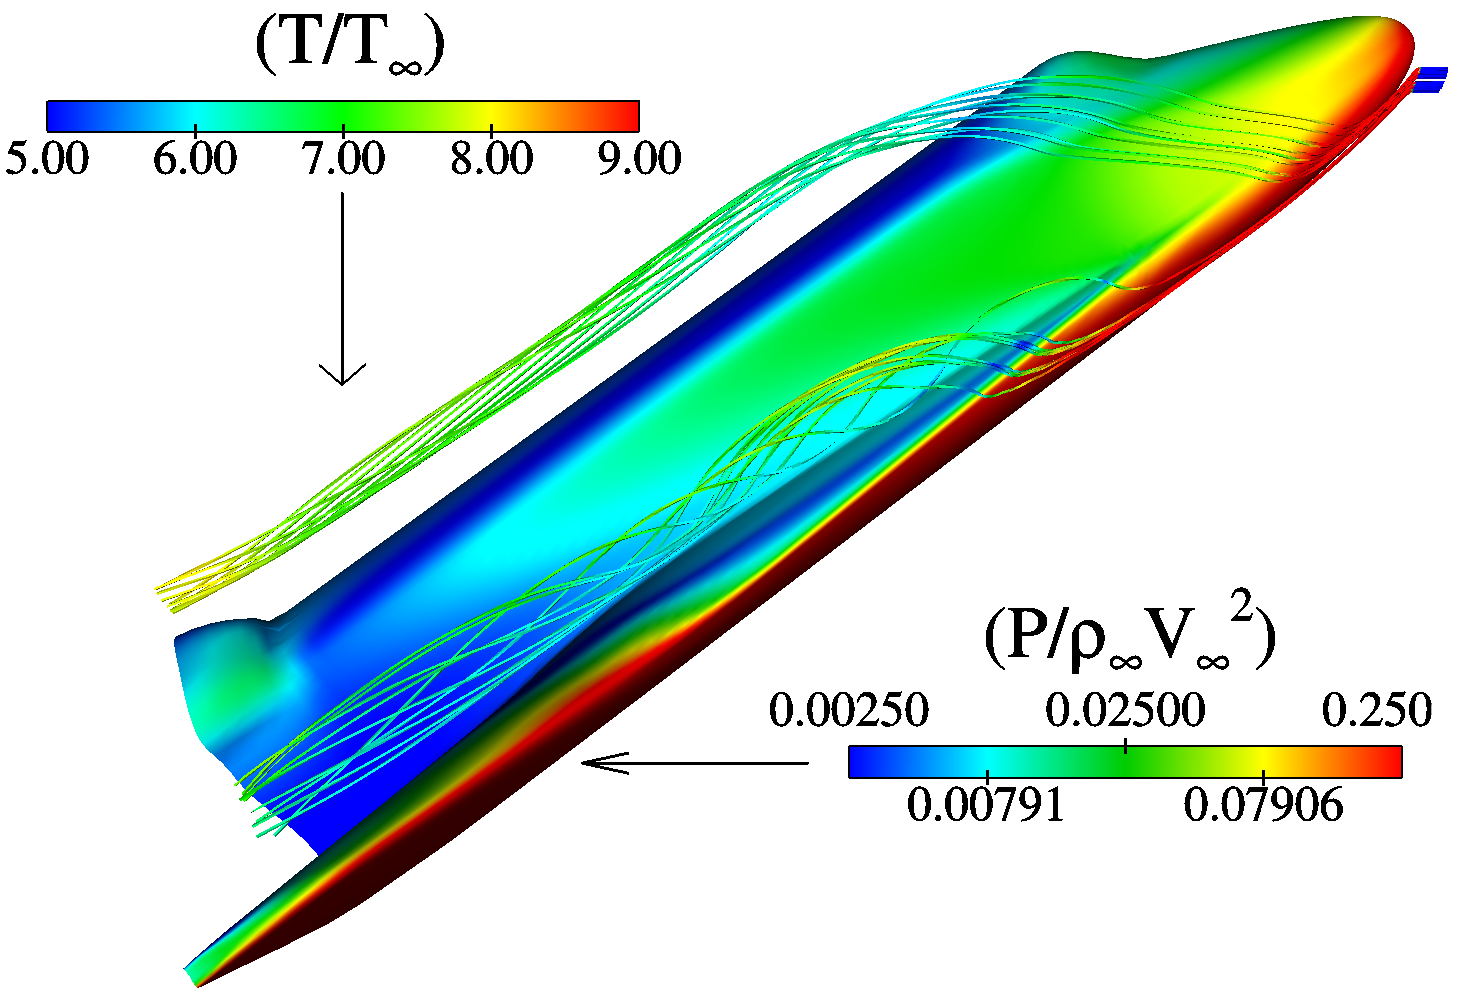
\includegraphics[width=.33\textwidth]{figures/orbiter/side_view_a35}
  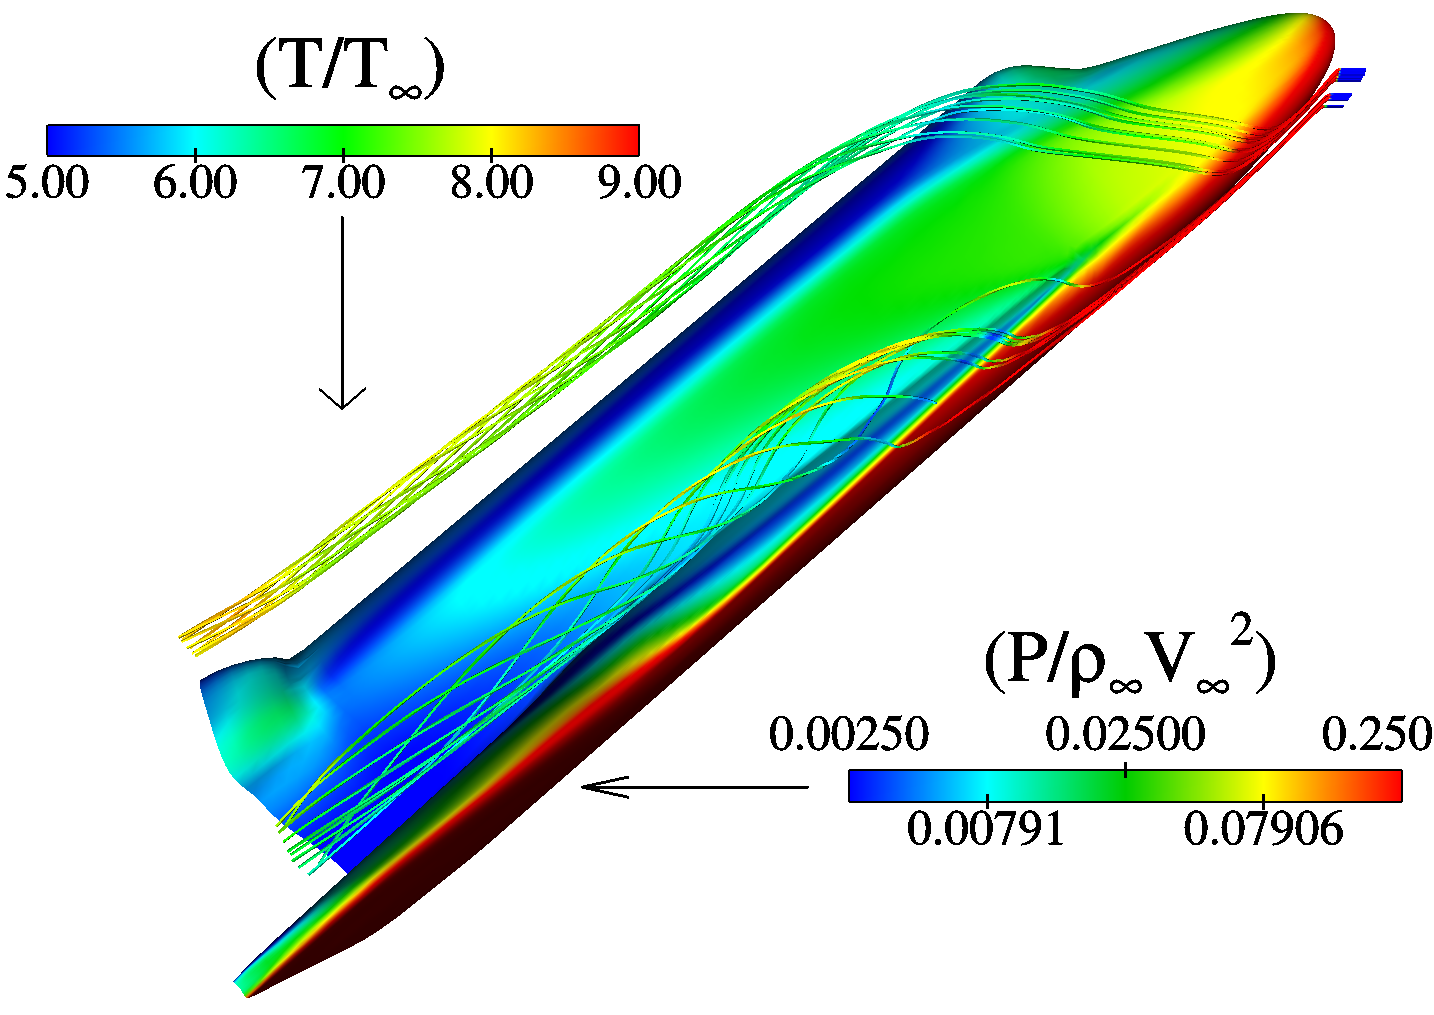
\includegraphics[width=.33\textwidth]{figures/orbiter/side_view_a40}

  \ldots is concerned with predicting aerodynamic forces on a vehicle which result predominantly from the surface pressure distribution, but also from viscous shear stress.
  \vspace{1em}

  Properly characterizing the aerodynamic performance of reentry vehicles is critical for optimal trajectory design.
}
 
\frame
{
  \frametitle{Aerothermodynamics}
  \begin{center}
    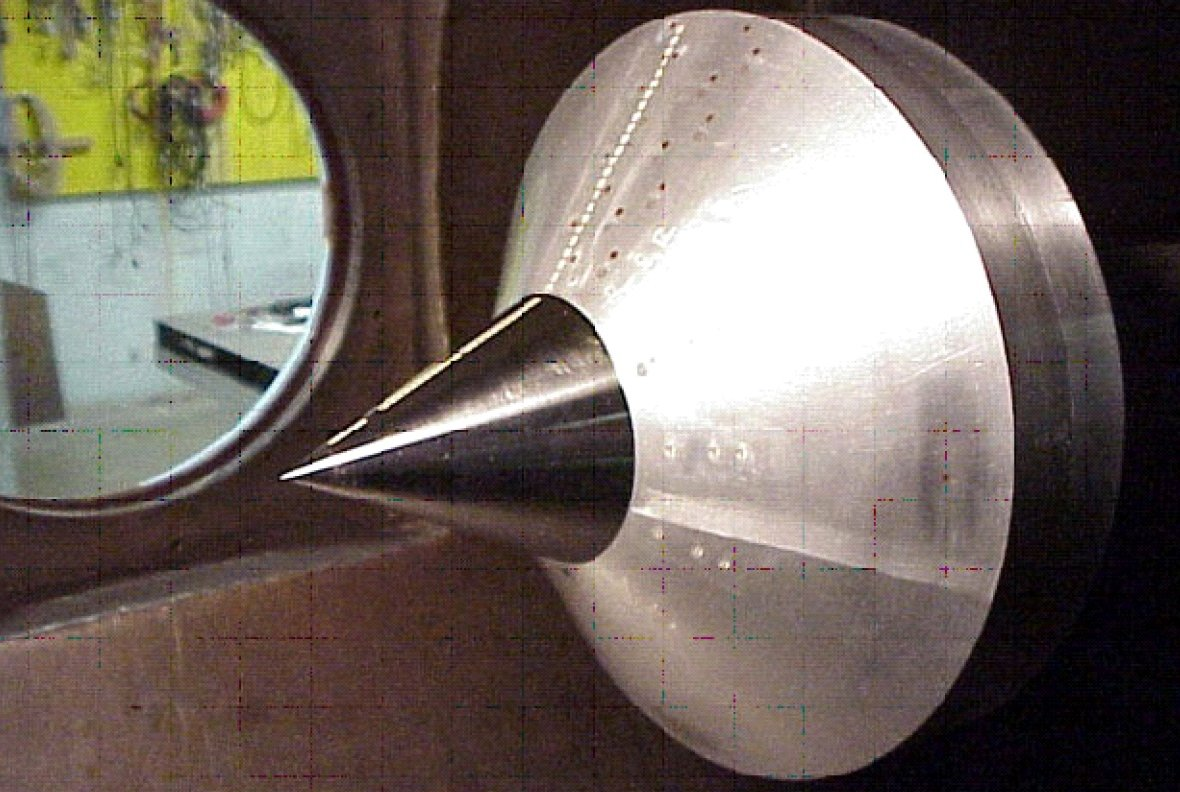
\includegraphics[height=.3\textheight]{figures/holden_double_cone/test_article}
    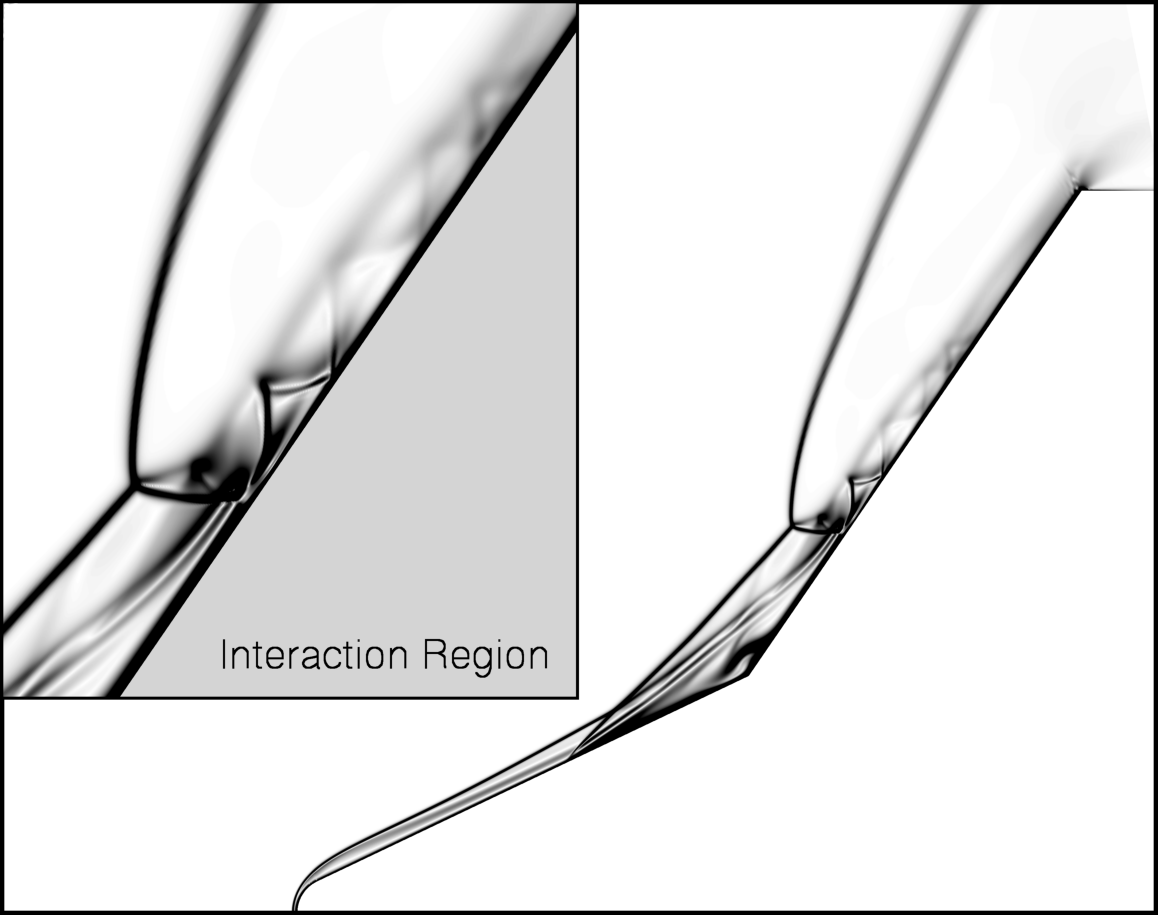
\includegraphics[height=.3\textheight]{figures/holden_double_cone/schlieren}
    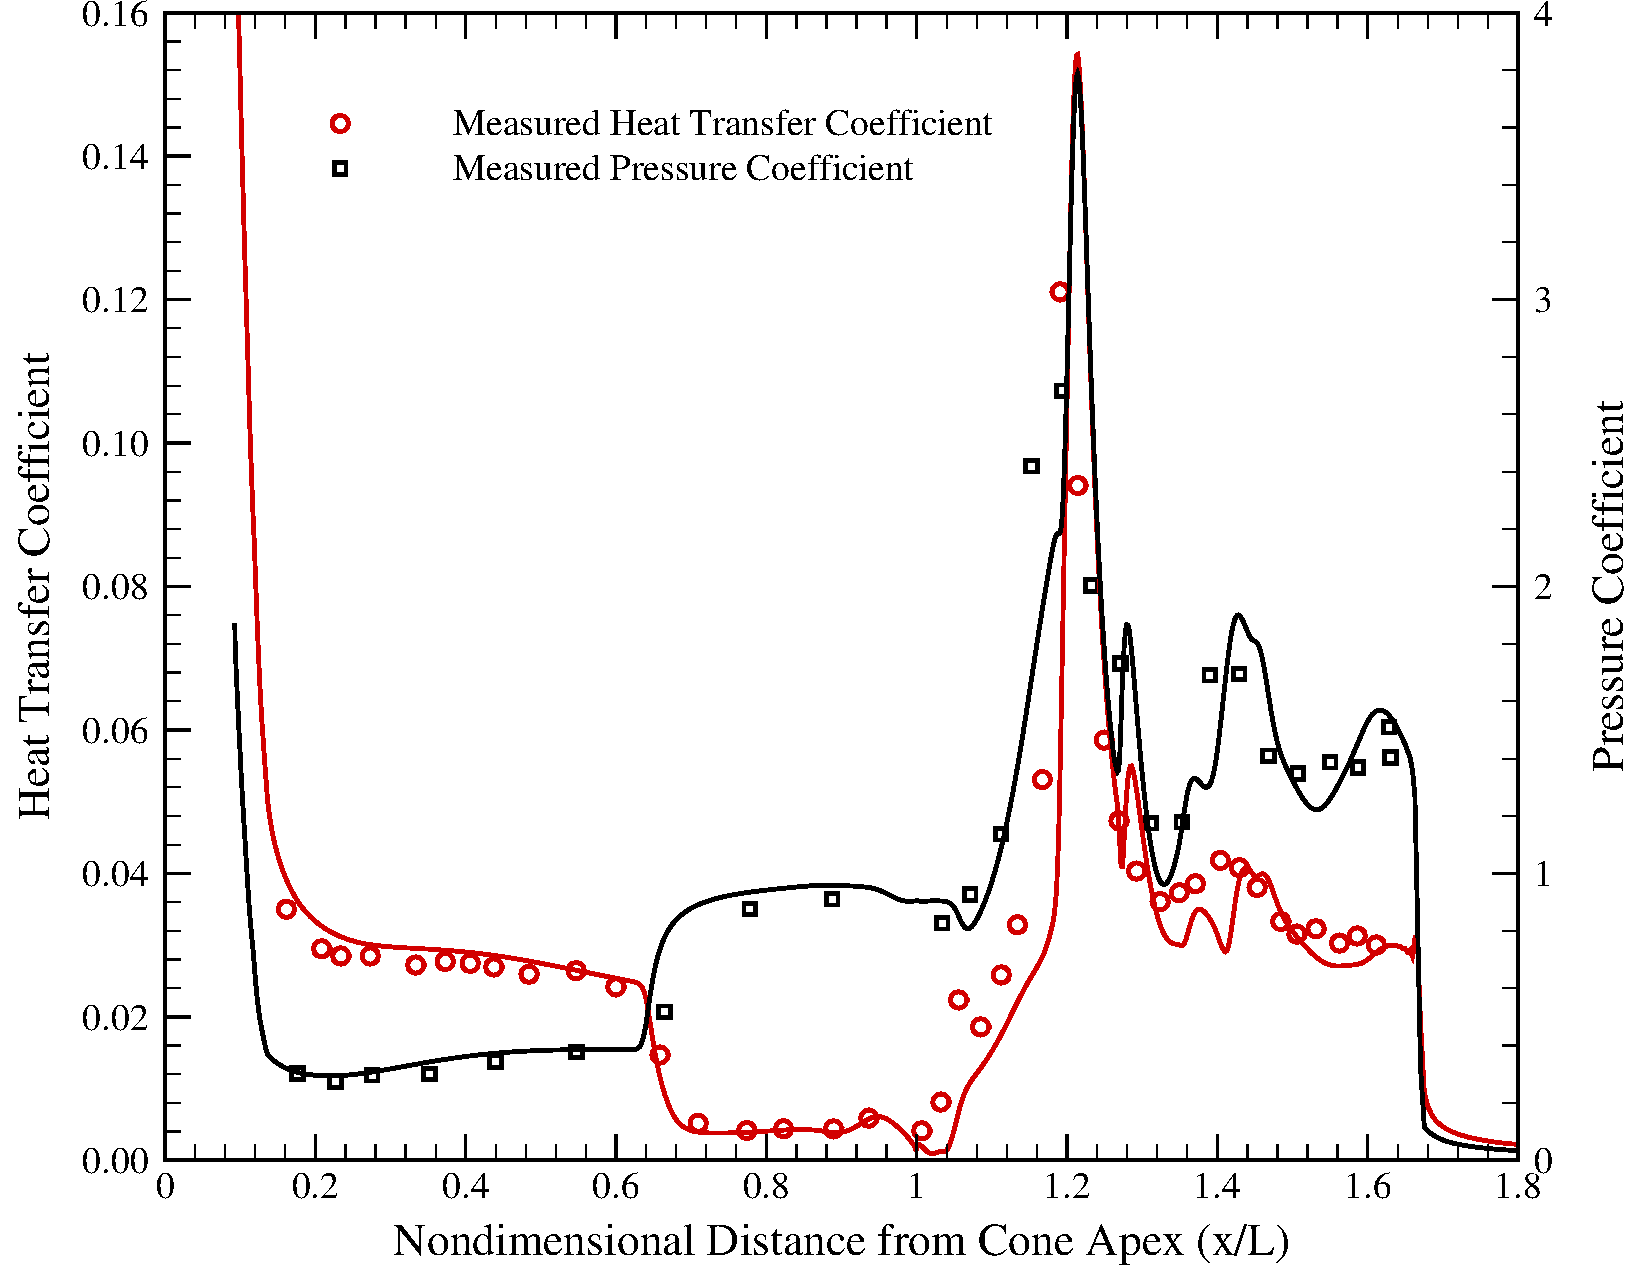
\includegraphics[height=.3\textheight]{figures/holden_double_cone/ch_cp_comparison}
  \end{center}
  
  \ldots is concerned with predicting the instantaneous total heat transfer rate and integrated heat load into a vehicle.
  \vspace{1em}

  Properly characterizing this environment is crucial because it provides the design conditions for the thermal protection system:
  \vspace{1em}
  
  \mbox{  }\textbf{heat transfer rate} $\rightarrow$ thermal protection material selection
  
  \mbox{  }\textbf{heat load} $\rightarrow$ thermal protection material thickness
}

\frame
{
  The primary goals of this presentation are:
  \vspace{.5em}
  
  \begin{enumerate}
    \item Present current research applying the Streamline Upwind Petrov-Galerkin Finite Element Method to aerothermodynamics applications
    \item Present validation studies comparing the developed numerical method with high-quality experimental data
    \item Identify potential collaboration 
  \end{enumerate}
}

\subsection{Governing Equations}
\frame
{
  The conservation of mass, momentum, and energy for a compressible fluid may be written as
  \begin{align}
    \label{eq:pde_comp_mass}
    \pdv{\rho}{t} &+ \grad{}\cdot \left(\rho\bv{u}\right) = 0 \\
    \label{eq:pde_comp_mom}
    \pdv{\rho\bv{u}}{t} &+ \grad{}\cdot\left(\rho\bv{u}\bv{u}\right) =
    -\grad{P} + \grad{}\cdot\bt{\tau} \\
    \label{eq:pde_comp_energy}
    \pdv{\rho E}{t} &+ \grad{}\cdot\left(\rho E \bv{u}\right) =
    -\grad{}\cdot\bv{q} - P\grad{}\cdot\bv{u} + \grad{}\cdot\left(\bt{\tau}\bv{u}\right)  
  \end{align}
  where $\rho$ is the density, $\bv{u}$ is the velocity, $E=e + \frac{\bv{u}\cdot\bv{u}}{2}$ is the total energy per unit mass, and $P$ is the pressure.
}

\frame
{
  \small
  The viscous stress tensor $\bt{\tau}$ and the heat flux vector $\bv{q}$ are defined as
  \begin{align}
    \label{eq:stress_tensor}
    \bv{\tau} &= \mu\left(\grad{\bv{u}} + \tgrad{\bv{u}}\right) + \lambda \left(\grad{}\cdot\bv{u}\right)\bt{I} \\
    \label{eq:fouriers_law}
    \bv{q} &= -k\grad{T}
  \end{align}
  where $\mu$ is the dynamic viscosity, $\lambda$ is the second coefficient of viscosity, $k$ is the thermal conductivity, and $T$ is the fluid temperature.  The two coefficients of viscosity are related to the bulk viscosity $\kappa$ by
  \begin{equation}
    \label{eq:bulk_viscosity}
    \kappa = \frac{2}{3} \mu + \lambda
  \end{equation}
  In general, the bulk viscosity is negligible except in detailed studies of shock wave structure or for investigations of the adsorption and attenuation of acoustic waves~\cite{cfmht}. Under this assumption, $\kappa=0$ in Equation~\eqref{eq:bulk_viscosity} and $\lambda$ is defined as
  \begin{equation}
    \label{eq:stokes_hypothesis}
    \lambda = -\frac{2}{3} \mu
  \end{equation}
  Equation~\eqref{eq:stress_tensor} with~\eqref{eq:stokes_hypothesis} is known as Stokes' hypothesis for a Newtonian fluid~\cite{panton_incompressible_flow}.
  \normalsize
}


\frame
{
  \begin{itemize}
    \item Provided the transport properties may be related to the unknowns, Equations~\eqref{eq:pde_comp_mass}--\eqref{eq:pde_comp_energy} form 5 equations in 7 unknowns (in three-dimensions).
    \item For a gas in thermodynamic equilibrium any two independent properties fix the state:
      \begin{equation*}
	T = T\left(\rho,e\right),\;\;\; P = P\left(\rho,e\right)
      \end{equation*}
    \item In the special case of a calorically perfect gas
      \begin{equation*}
	c_v T = e,\;\;\; P = \rho e\left(\gamma-1\right)
      \end{equation*}
  \end{itemize}
}

\frame
{
  \frametitle{\scriptsize High-Temperature Gas Dynamics}
  \begin{itemize}
      
  \item For the case of thermochemical nonequilibrium the equation set is enlarged to contain
      \begin{itemize}
	\item Local mass balance statements for constituent species.  That is,
	  \begin{equation*}
	    \pdv{\rho}{t} + \grad{}\cdot\rho \bv{u} = 0 
	  \end{equation*}
	  becomes
	  \begin{equation*}
	    \pdv{\rho_s}{t} + \grad{}\cdot\left(\rho_s \bv{u} - \bv{J}_s\right) = \omega_s 
	  \end{equation*}	  
	\item Local energy balance/exchange statements for internal modes.  That is, the ``temperature'' is no longer well defined. Must account for $T,T_r,T_v,T_e$ modes.  Usually done with a \emph{two temperature} model.
      \end{itemize}
    \item For a weakly ionized gas, becomes a set of 11+3+2 coupled, reacting  equations.
    \item At superorbital reentry velocities (above \unitfrac[10]{km}{sec}) must also account for radiative heat transfer.
	  
  \end{itemize}
}

\frame
{
  In the literature equations~\eqref{eq:pde_comp_mass}--\eqref{eq:pde_comp_energy} are often treated as the system\footnote{\tiny the notation is cumbersome, but it is fairly standard}
  \begin{equation}
    \label{eq:pde_comp}
    \pdv{\bv{U}}{t} + \pdv{\bv{F}_i}{x_i} = \pdv{\bv{G}_i}{x_i}
  \end{equation}
  which can be written in terms of the unknowns $\bv{U}=\left[\rho, \rho u, \rho v, \rho w, \rho E\right]^T$ as
  \begin{equation}
    \label{eq:pde_comp2}
    \pdv{\bv{U}}{t} + \bt{A}_i \pdv{\bv{U}}{x_i} =
    \pdv{}{x_i} \left( \bt{K}_{ij} \pdv{\bv{U}}{x_j} \right)
  \end{equation}
  where $\bt{A}_i = \pdv{\bv{F}_i}{\bv{U}}$ is the inviscid flux Jacobian, and the viscous flux vector $\bv{G}_i$ may be written as
  \begin{equation}
    \label{eq:viscous_flux_jacobian}
    \pdv{\bv{G}_i}{x_i} = \pdv{}{x_i} \left( \bt{K}_{ij} \pdv{\bv{U}}{x_j} \right)
  \end{equation}
  \normalsize
}

%% \frame
%% {
%%   \begin{itemize}
%%     \item  The choice of the \emph{conserved variables} $\bv{U}=\left[\rho, \rho u, \rho v, \rho w, \rho E\right]^T$ is convenient for high-speed compressible flows ($M\gtrsim 0.3$) as it allows for explicit algorithms for~\eqref{eq:pde_comp2}.
%%     \item Other choices are possible which have applicability to a larger range of flow problems~\cite{hauke_hughes_compressible_variables}
%%     \item Equation~\eqref{eq:pde_comp2}  may be transformed for any set of variables $\bv{V}$ via $\bv{U}= \bt{A}_0 \bv{V}$ where $\bt{A}_0\equiv\pdv{\bv{U}}{\bv{V}}$.
%%     \item Ease of applying boundary conditions varies widely with variable choice
%%   \end{itemize}
%%   \normalsize
%% }

%% \subsection{Godunov's Theorem}
%% \frame
%% {
%%   Godunov's theorem~\cite{godunov} is particularly relevant for numerical methods applied to high-speed gas dynamics:
%%   \begin{quote}
%%     Any linear monotone scheme cannot be better than first-order accurate. 
%%   \end{quote}
%%   For the model linear convection-diffusion problem
%%   \begin{equation}
%%     \nonumber
%%     -\varepsilon \Delta u + \bv{v}\cdot\grad{u} = f
%%   \end{equation}
%%   with $\bv{v}$ specified independently of $u$ this implies that \emph{even for linear problems}, a monotone second-order (or higher) scheme \emph{is necessarily nonlinear}.
%%   This has important implications going forth on the interplay between upwinding, shock capturing, and solution limiting.
%% }

\section[SUPG FEM]{SUPG Galerkin Finite Element Methods}
\frame
{
  \vspace{4em}
  \centerline{\huge{The Streamline-Upwind Petrov-Galerkin}}
  \vspace{.5em}

  \centerline{\huge{Finite Element Method}}
}

\subsection{Weak Formulation}
\frame
{
  \vspace{-1.5em}
  \small
  Upwinding is required to stabilize convection-dominated flows. In SUPG schemes this is accomplished by biasing the test functions $\hat{\bv{W}}$ in the upstream direction:
  \begin{equation}
     \hat{\bv{W}} = \bv{W} + \bt{\tau}_{SUPG}\;\bt{A}_i\pdv{\bv{W}}{x_i}
  \end{equation}
  \uncover<2->
   {
   	Standard Galerkin treatment \& SUPG-upwinding applied to~\eqref{eq:pde_comp2} to produce the stabilized weak form: \emph{find $\bv{U}$ such that}
   	\begin{eqnarray}
   	  \label{eq:comp_weak_SUPG}
   	  \int_\Omega  \left[ \bv{W}\cdot\left(\pdv{\bv{U}}{t} + \bt{A}_i \pdv{\bv{U}}{x_i} \right) + \pdv{\bv{W}}{x_i} \cdot \left( \bt{K}_{ij} \pdv{\bv{U}}{x_j} \right) \right] \dx \nonumber \\
   	  + \sum_{e=1}^{n_{el}} \int_{\Omega_e} \bt{\tau}_{SUPG} \pdv{\bv{W}}{x_k}\cdot\bt{A}_k
   	  \left[ \pdv{\bv{U}}{t} + \bt{A}_i \pdv{\bv{U}}{x_i} - \pdv{}{x_i} \left( \bt{K}_{ij} \pdv{\bv{U}}{x_j} \right) \right] \dx  \nonumber \\
   	  = \int_\Gamma \bv{W}\cdot\bv{g} \ds
   	\end{eqnarray}
   	\emph{for all $\bv{W}$ in an appropriate function space}.
   	\vspace{.5em}
  
   	For compressible flows $\bt{\tau}_{SUPG}$ is generally diagonal~\cite{hauke_hughes_compressible_variables}.
   }
}

\subsection{Shock Capturing}
\frame
{
  \small
  SUPG stabilization does not yield monotone solutions.  Additional treatment is needed to prevent spurious oscillations in regions of shockwaves.  Hence~\eqref{eq:comp_weak_SUPG} is augmented with a \emph{shock capturing} term to produce the augmented weak form: \emph{find $\bv{U}$ such that}
  \begin{eqnarray}
  \label{eq:comp_weak_SUPG_SC}
  \int_\Omega  \left[ \bv{W}\cdot\left(\pdv{\bv{U}}{t} + \bt{A}_i \pdv{\bv{U}}{x_i} \right) + \pdv{\bv{W}}{x_i} \cdot \left( \bt{K}_{ij} \pdv{\bv{U}}{x_j} \right) \right] \dx \nonumber \\
  + \sum_{e=1}^{n_{el}} \int_{\Omega_e} \bt{\tau}_{SUPG} \pdv{\bv{W}}{x_k}\cdot\bt{A}_k
  \left[ \pdv{\bv{U}}{t} + \bt{A}_i \pdv{\bv{U}}{x_i} - \pdv{}{x_i} \left( \bt{K}_{ij} \pdv{\bv{U}}{x_j} \right) \right] \dx  \nonumber \\
  + \sum_{e=1}^{n_{el}} \int_{\Omega_e} \delta \left(\pdv{\bv{W}}{x_i}\cdot\pdv{\bv{U}}{x_i}\right)\dx
   = \int_\Gamma \bv{W}\cdot\bv{g} \ds
\end{eqnarray}
  \emph{for all $\bv{W}$ in an appropriate function space}.
  \vspace{.5em}
  
  $\delta$ in this work is modified from~\cite{gjlebeau_thesis,skaliabadi_dissertation}.  Note that discretizations of~\eqref{eq:comp_weak_SUPG_SC} reduce to $\mathcal{O}(h)$ in regions of appreciable~$\delta$.
  \normalsize  
}

\frame
{
  \small
  The shock capturing operator, $\delta$, was adapted for a system of conservation variables by LeBeau and Tezduyar~\cite{gjlebeau_thesis,skaliabadi_dissertation,aliabadi_tezduyar_IJNMF_1995} from the original definition employed by Hughes et al.\ for the case of entropy variables~\cite{hughes_shock_capturing,shakib_hughes_ns}.  A modified form is employed in the present work and is defined as
\begin{equation}
  \label{eq:shock_capturing_parameter}
  \delta = \left[\frac{\left\|\pdv{\bv{U}}{t} + \bt{A}_i\pdv{\bv{U}}{x_i}
                       - \pdv{}{x_i} \left( \bt{K}_{ij} \pdv{\bv{U}}{x_j} \right)\right\|_{\bt{A}_0^{-1}}}
                      {\|\grad{\xi}  \cdot\grad{\bv{U}}\|_{\bt{A}_0^{-1}} +
		       \|\grad{\eta} \cdot\grad{\bv{U}}\|_{\bt{A}_0^{-1}} +
		       \|\grad{\zeta}\cdot\grad{\bv{U}}\|_{\bt{A}_0^{-1}}}\right]^{1/2}
\end{equation}
where $\left(\xi,\eta,\zeta\right)$ are the canonical reference element coordinates and $\bt{A}_0^{-1}$ is the mapping from conservation to entropy variables.
\vspace{.5em}

In this work the numerator is modified from its original form to retain consistency with~\eqref{eq:pde_comp2} in the case of transient, viscous flows.
}

\subsection{Inviscid Flux Discretization}
\frame
{
  \scriptsize
  Expand $\bv{U}(\bv{x},t)$ and $\bv{F}_i(\bv{x},t)$ in terms of standard Lagrange finite element basis functions:
  \begin{align}
    \bv{U}  (\bv{x},t) &= \sum_j \phi_j(\bv{x}) \bv{U}(\bv{x}_j,t)   \label{eq:disc_U_expanded} \\
    \bv{F}_i(\bv{x},t) &= \sum_j \phi_j(\bv{x}) \bv{F}_i(\bv{x}_j,t) \label{eq:disc_F_expanded}
  \end{align}
  where $\bv{U}(\bv{x}_j,t)$ and $\bv{F}_i(\bv{x}_j,t)=\bt{A}_i\left(\bv{U}\left(\bv{x}_j,t\right)\right)\bv{U}(\bv{x}_j,t)$ are the nodal solution inviscid flux values at time $t$. A standard piecewise linear Lagrange basis is chosen for $\{\phi\}$ (yielding a nominally 2\textsuperscript{nd}--order accurate scheme).

  \uncover<2->
  {
    This approach is in contrast to previous SUPG discretizations for compressible flows.~\cite{gjlebeau_thesis,skaliabadi_dissertation,hauke_hughes_compressible_variables,catabriga_coutinho_SUPG_convergence}
    \begin{align}
      \bv{F}_i(\bv{x},t) &= \sum_j \phi_j(\bv{x}) \bv{F}_i(\bv{x}_j,t) \nonumber \\
      &= \sum_j \phi_j(\bv{x}) \bt{A}_i\left(\bv{U}\left(\bv{x}_j,t\right)\right)\bv{U}(\bv{x}_j,t) \label{eq:disc_F=AU_expanded}
    \end{align}
  }
  
  \uncover<3->
  {
    contrasts to the typical approach in which
    \begin{equation}
      \bv{F}_i(\bv{x},t) = \bt{A}_i\left(\bv{U}\left(\bv{x},t\right)\right)\bv{U}(\bv{x},t) \label{eq:disc_F=AU_expanded_standard}
    \end{equation}
    where $\bv{U}(\bv{x},t)$ is interpolated from nodal values as in~\eqref{eq:disc_U_expanded}.
  }
}

\frame
{
  \small
  Consider a one-dimensional, inviscid, normal shock at Mach~5.  For this simple case the governing equations reduce to
  \begin{align*}
    \pdv{\rho}{t} &+ \pdv{}{x} \left(\rho u\right) = 0 \\
    \pdv{\rho u}{t} &+ \pdv{}{x}\left(\rho u^2 + P\right) = 0 \\
    \pdv{\rho E}{t} &+ \pdv{}{x} \left(\rho u H\right) = 0
  \end{align*}
  and, at steady state, become
  \begin{equation}
    \pdv{}{x} \left(\rho u\right) = \pdv{}{x} \left(\rho u^2 + P\right) = \pdv{}{x} \left(\rho u H\right) \equiv 0 \label{eq:1d_steady_NS}
  \end{equation}
  which implies that $\rho u$, $\rho u^2+P$, and $\rho u H$ are all constant.
}

\frame
{
  \frametitle{\scriptsize Comparison between reconstructed and interpolated inviscid flux discretizations}
  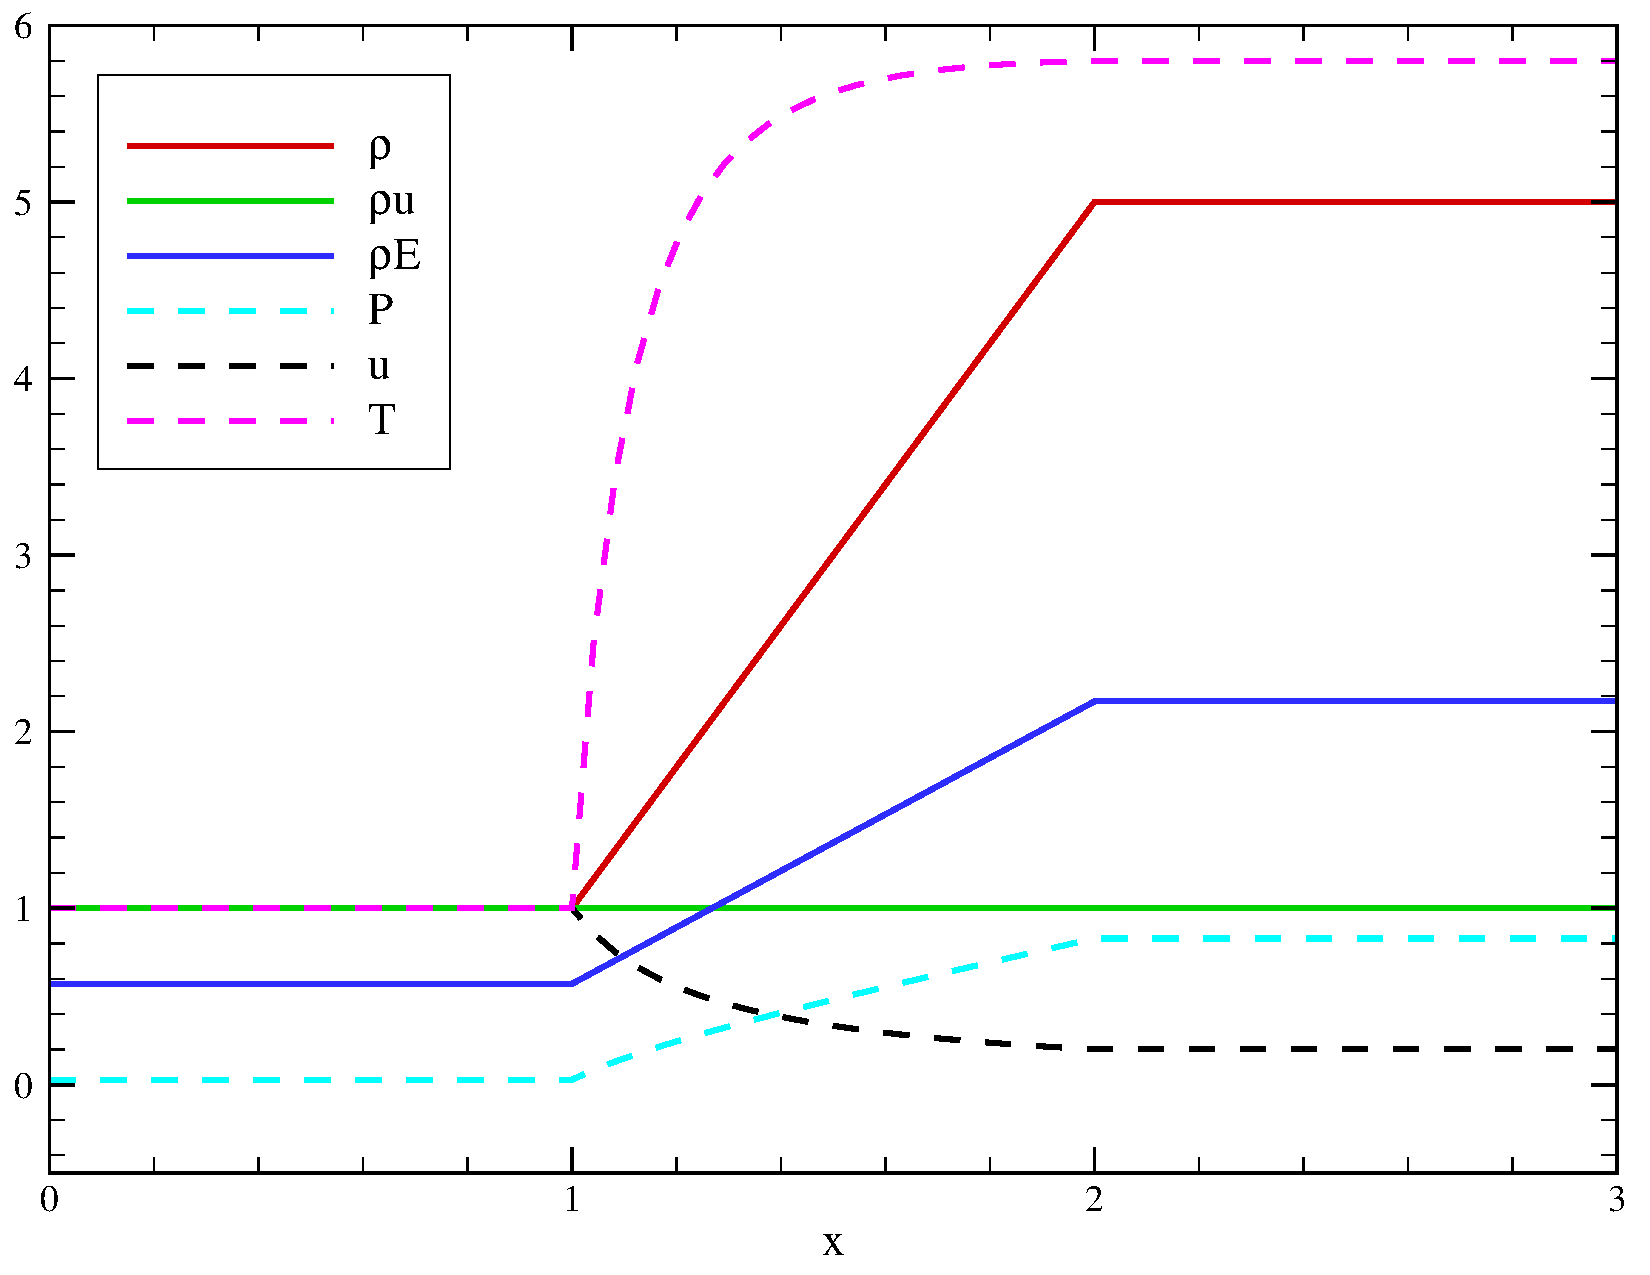
\includegraphics[width=.48\textwidth]{figures/comp_ns_interpolation/primitive_vars}
  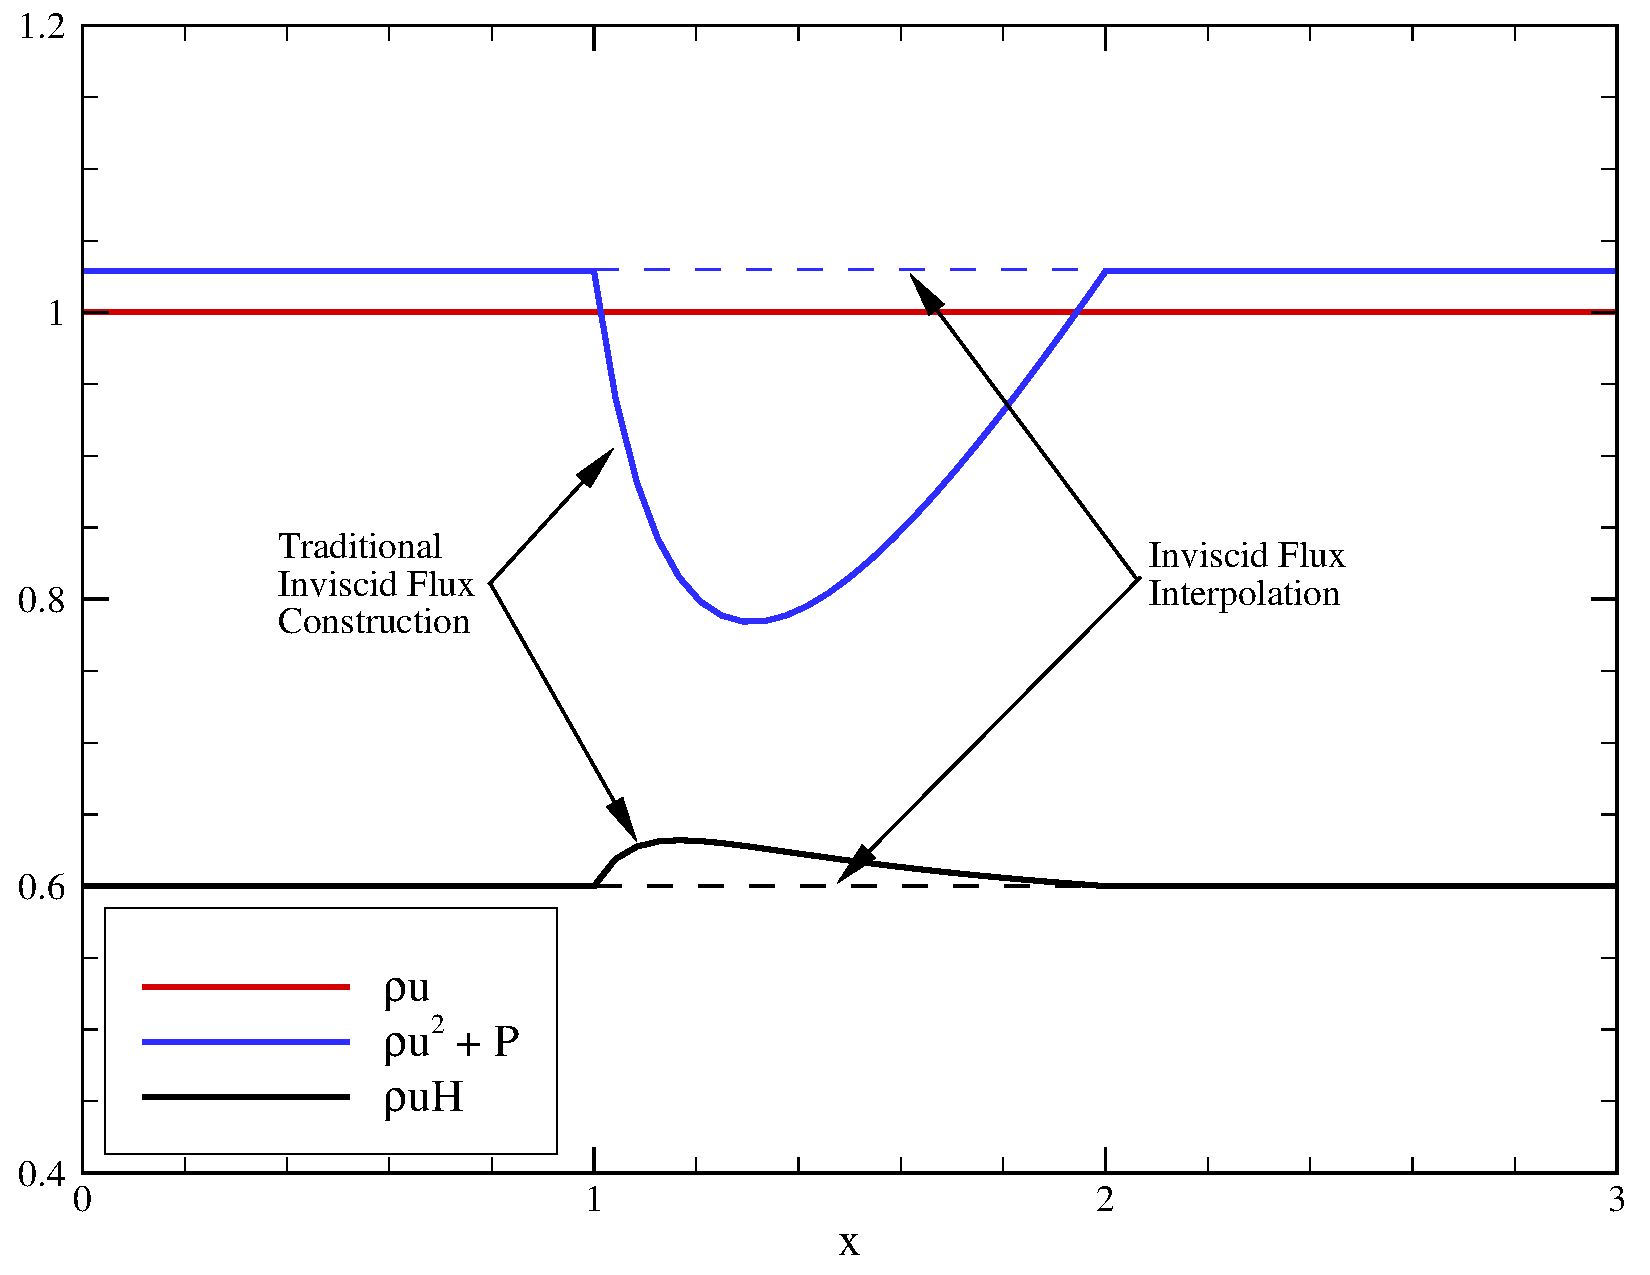
\includegraphics[width=.48\textwidth]{figures/comp_ns_interpolation/inv_flux}
}

\subsection{Time Discretization}
\frame
{
  \scriptsize
  The semidiscrete weak form in equation~\eqref{eq:comp_weak_SUPG_SC} is discretized in time using a backwards finite difference scheme.  Both first and second-order accurate in time schemes may be derived from Taylor series expansions in time about $\bv{U}_{n+1}$:
  
  \uncover<2->
  {
    \begin{align}
      \bv{U}_n     = \bv{U}_{n+1} &+ \pdv{\bv{U}_{n+1}}{t}\left(t_n-t_{n+1}\right) + \pdtwov{\bv{U}_{n+1}}{t}\frac{\left(t_n-t_{n+1}\right)^2}{2} \nonumber \\
      &+ \mathcal{O}\left(\left(t_n-t_{n+1}\right)^3\right) \nonumber \\
      & \nonumber \\
      \bv{U}_{n-1} = \bv{U}_{n+1} &+ \pdv{\bv{U}_{n+1}}{t}\left(t_{n-1}-t_{n+1}\right) + \pdtwov{\bv{U}_{n+1}}{t}\frac{\left(t_{n-1}-t_{n+1}\right)^2}{2} \nonumber \\
      &+ \mathcal{O}\left(\left(t_{n-1}-t_{n+1}\right)^3\right) \nonumber
    \end{align}
  }
      
  \uncover<3->
  {
    which, upon substituting $t_{n+1} - t_n\equiv\Delta t_{n+1}$ and $t_{n+1} - t_{n-1}=\Delta t_{n+1} + \Delta t_n$, becomes
    \begin{align}
      \bv{U}_n     = \bv{U}_{n+1} &- \pdv{\bv{U}_{n+1}}{t}\Delta t_{n+1} + \pdtwov{\bv{U}_{n+1}}{t}\frac{\Delta t_{n+1}^2}{2} - \mathcal{O}\left(\Delta t_{n+1}^3\right) \nonumber \\ 
      & \nonumber \\
      \bv{U}_{n-1} = \bv{U}_{n+1} &- \pdv{\bv{U}_{n+1}}{t}\left(\Delta t_{n+1}+\Delta t_n\right) + \pdtwov{\bv{U}_{n+1}}{t}\frac{\left(\Delta t_{n+1}+\Delta t_n\right)^2}{2} \nonumber \\
      &- \mathcal{O}\left(\left(\Delta t_{n+1}+\Delta t_n\right)^3\right) \nonumber
    \end{align}
  }
}

\frame
{
  \scriptsize
  Which can be rewritten for $\pdv{\bv{U}_{n+1}}{t}$ as:
  \begin{align}
    \pdv{\bv{U}_{n+1}}{t} = &\frac{\bv{U}_{n+1}}{\Delta t_{n+1}} - \frac{\bv{U}_n}{\Delta t_{n+1}} + \pdtwov{\bv{U}_{n+1}}{t} \frac{\Delta t_{n+1}}{2}
    - \mathcal{O}\left(\Delta t_{n+1}^2\right) \label{eq:udot,un} \\
    & \nonumber \\
    \pdv{\bv{U}_{n+1}}{t} = &\frac{\bv{U}_{n+1}}{\Delta t_{n+1} + \Delta t_n} - \frac{\bv{U}_{n-1}}{\Delta t_{n+1} + \Delta t_n} + \pdtwov{\bv{U}_{n+1}}{t}\frac{\left(\Delta t_{n+1} + \Delta t_n\right)}{2} \nonumber \\
    &- \mathcal{O}\left(\left(\Delta t_{n+1} + \Delta t_n\right)^2\right) \label{eq:udot,unm1}
  \end{align}
}

\subsubsection{Time Marching to Steady State}
\frame
{
  The familiar backwards Euler time discretization follows directly from~\eqref{eq:udot,un} by recognizing
\begin{equation}
  \pdv{\bv{U}_{n+1}}{t} = \frac{\bv{U}_{n+1}-\bv{U}_n}{\Delta t_{n+1}} + \mathcal{O}\left(\Delta t_{n+1}\right)
  \label{eq:udot_backward_euler}
\end{equation}
which provides a first-order in time approximation upon neglecting the $\mathcal{O}\left(\Delta t_{n+1}\right)$ term.
}

\subsubsection{Time-Accurate Flows}
\frame
{
  \vspace{-.5em}
  \scriptsize
  A linear combination of $\left(1+\frac{\Delta t_{n+1}}{\Delta t_n}\right)\times$\eqref{eq:udot,un} and $-\frac{\Delta t_{n+1}}{\Delta t_n}\times$\eqref{eq:udot,unm1} can be used to annihilate the leading $\pdtwov{\bv{U}_{n+1}}{t}$ term to create a backwards, second-order accurate approximation to $\pdv{\bv{U}_{n+1}}{t}$.
  \vspace{.5em}
  
  This approximation, along with~\eqref{eq:udot_backward_euler}, can be generalized in the form
  \begin{equation}
    \pdv{\bv{U}_{n+1}}{t} = \alpha_t \bv{U}_{n+1} + \beta_t \bv{U}_n + \gamma_t \bv{U}_{n-1} + \mathcal{O}\left(\Delta t_{n+1}^p\right)
    \label{eq:udot_thee_pt_backward}
  \end{equation}
  to yield either a first or second-order accurate scheme.  The weights $\alpha_t, \beta_t$, and $\gamma_t$ are given below for $p=1$ and $p=2$.

  \normalsize
  \begin{center}
    \begin{tabular}{c||ccc}
      $\bv{p}$ & $\bv{\alpha_t}$ & $\bv{\beta_t}$ & $\bv{\gamma_t}$ \\ \hline\hline
          &          &         & \\
       1  & $\frac{1}{\Delta t_{n+1}}$ & $\frac{-1}{\Delta t_{n+1}}$ & 0 \\
          &          &         & \\
       2  & $-\beta_t - \gamma_t$ %$\left[\frac{1}{\Delta t_{n+1}} + \frac{1}{\Delta t_n} - \frac{\Delta t_{n+1}}{\Delta t_n\left(\Delta t_n+1 + \Delta t_n\right)}\right]$ 
          & $-\left[\frac{1}{\Delta t_{n+1}} + \frac{1}{\Delta t_n}\right]$
          & $\frac{\Delta t_{n+1}}{\Delta t_n\left(\Delta t_{n+1} + \Delta t_n\right)}$ 
    \end{tabular}
  \end{center}
}

\frame
{
  \frametitle{\scriptsize Time Step Selection}
  \vspace{-1em}
  \footnotesize
  The simulation begins with the domain initialized to freestream conditions everywhere and a user-specified initial time step $\Delta t_0$ is used to advance the solution.  The time step then grows geometrically with the relative change in the unsteady residual measured over $k$ time steps.  Explicitly, 
\begin{align}
  \Delta \bar{t}_{n+1} &= \Delta t_{n-k} \max\left(\left[\frac{\mathcal{R}_{n-k}}{\mathcal{R}_{n}}\right]^r,1\right) \label{geometric_timestep_growth} \\ \vspace{1em}
                 & \nonumber \\
  \Delta t_{n+1} &= \min\left(\Delta \bar{t}_{n+1},\Delta t_{\text{max}}\right) \label{dt_limiting}
\end{align}
where $\mathcal{R}_{n} \equiv \left\|\frac{\Delta \bv{U}_n}{\Delta t}\right\|_{\infty}$ and $r=1.2$ is the geometric growth rate.  The time step size is updated every $k=5$ time steps.
\vspace{1em}

Typically the maximum allowable time step for steady problems is $\Delta t_{\text{max}}=1$, which corresponds to the amount of time required for a fictitious point in the freestream to be convected one reference length.

}


\subsection{Linearization}
\frame
{
  After temporal \& spatial discretization,  Equation~\eqref{eq:comp_weak_SUPG_SC} can be written in residual form for the unknown nodal values $\bv{U}_{n+1}\equiv\bv{U}_h\left(t_{n+1}\right)$ as the nonlinear algebraic system
\begin{equation}
  \label{eq:comp_residual}  
  \bv{R}\left(\bv{U}_{n+1}\right) = 0 
\end{equation}
We seek to define a sequence of linear problems $\left\{\bv{U}_{n+1}^l\right\}$ that converge to $\bv{U}_{n+1}$, the solution of~\eqref{eq:comp_residual}.
}

\frame
{
  \frametitle{\scriptsize Newton Scheme}
  \vspace{-1em}
  \footnotesize
  Expanding~\eqref{eq:comp_residual} with a Taylor series about iterate $\bv{U}_{n+1}^l$ gives
  \begin{equation}
    \label{eq:comp_residual_linearized}  
    \bv{R}\left(\bv{U}_{n+1}^{l+1}\right) = \bv{R}\left(\bv{U}_{n+1}^l\right) +\left[\pdv{\bv{R}\left(\bv{U}_{n+1}^l\right)}{\bv{U}_{n+1}}\right]\;\delta\bv{U}_{n+1}^{l+1} + \mathcal{O}\left(\left(\delta\bv{U}_{n+1}^{l+1}\right)^2\right)
  \end{equation}
  where $\pdv{\bv{R}}{\bv{U}}$ is the Jacobian matrix for the nonlinear system and $\delta \bv{U}_{n+1}^{l+1}=\bv{U}_{n+1}^{l+1}-\bv{U}_{n+1}^l$.
  \vspace{1em}
  
  \uncover<2->
  {
    Truncating this expansion and setting $\bv{R}\left(\bv{U}_{n+1}^{l+1}\right)=0$ yields Newton's method:
    \begin{align}
      0 &= \bv{R}\left(\bv{U}_{n+1}^l\right) + \left[\pdv{\bv{R}\left(\bv{U}_{n+1}^l\right)}{\bv{U}_{n+1}}\right]\;\delta\bv{U}_{n+1}^{l+1} \nonumber \\
      \left[\pdv{\bv{R}\left(\bv{U}_{n+1}^l\right)}{\bv{U}_{n+1}}\right]\;\delta\bv{U}_{n+1}^{l+1} &= -\bv{R}\left(\bv{U}_{n+1}^l\right) \label{eq:comp_newton_system}
    \end{align}
  }
}

\frame
{
  \frametitle{\scriptsize Newton Scheme -- Comments}
  \vspace{-.5em}
  
  \begin{itemize}
    \item Newton's method exhibits second-order \emph{conditional} convergence
    \item Even for a calorically perfect gas, full Newton implementation is complicated by the nonlinear transport properties and convective terms
    \item Asymptotic convergence rate is rarely achieved for flows with strong shocks
    \item Computational cost of full-Newton may be mitigated with an approximate Newton-Krylov technique which accounts for the action of the Jacobian matrix in~\eqref{eq:comp_newton_system} without explicitly forming it
    \item This approach is especially attractive for ``real gas'' flows
  \end{itemize}
}

\frame
{
  \frametitle{\scriptsize Newton-Krylov Techniques}
  \vspace{-1em}
  \footnotesize
  
  \begin{itemize}
    \item The resulting sparse implicit linear systems are amenable to solution with iterative Krylov subspace techniques
    \item The kernel operation for such methods is the \emph{action} of a matrix-vector product.  That is, solving
      \begin{equation*}
	\bt{K} \bv{u} = \bv{f}
      \end{equation*}
      requires repeated computations of $\bv{w}=\bt{K}\bv{v}$
    \item For the Newton linearization,
      \begin{equation*}
	\left[\pdv{\bv{R}}{\bv{U}}\right]\;\delta\bv{U} = -\bv{R}\left(\bv{U}\right)
      \end{equation*}
      and the required matrix-vector product is of the form $\bv{w}=\left[\pdv{\bv{R}}{\bv{U}}\right]\bv{v}$, which is simply the derivative of $\bv{R}$ in the direction of $\bv{v}$
    \item This may be approximated via differencing residual evaluations, yielding a so-called matrix-free method:
      \begin{equation*}
	\bv{w} = \left[\pdv{\bv{R}}{\bv{U}}\right]\;\bv{v} \approx \frac{\bv{R}\left(\bv{U} + \varepsilon \bv{v}\right) - \bv{R}\left(\bv{U}\right)}{\varepsilon}
	\label{eq:comp_linsolve_mf}
      \end{equation*}
  \end{itemize}
}

\subsection{Implicit Solution Strategies}
\frame
{
  \vspace{-1.5em}
  \begin{columns}[t]
    \column{.6\textwidth}
    \begin{block}{}
      \footnotesize
      \begin{itemize}
        \item Time-marching to steady-state is almost always used for high-speed flows
	\item Implicit techniques required for viscous problems with tight wall spacing (also for stiff chemistry in the case of nonequilibrium)
	\item For steady problems, at each time step the resulting nonlinear problem is usually solved only approximately (usually 1 Newton step)
	\item DOF coupling defined via standard finite element basis function support determines sparse matrix structure
	\item Matrix-free GMRES with block-diagonal preconditioning used in earlier work~\cite{skaliabadi_dissertation}
	\item This work uses matrix \& matrix-free GMRES with full ILU-0 preconditioning -- \emph{linearization is important}
      \end{itemize}
    \end{block}
    \column{.4\textwidth}
    \begin{block}{}
      \tiny
      \begin{center}
	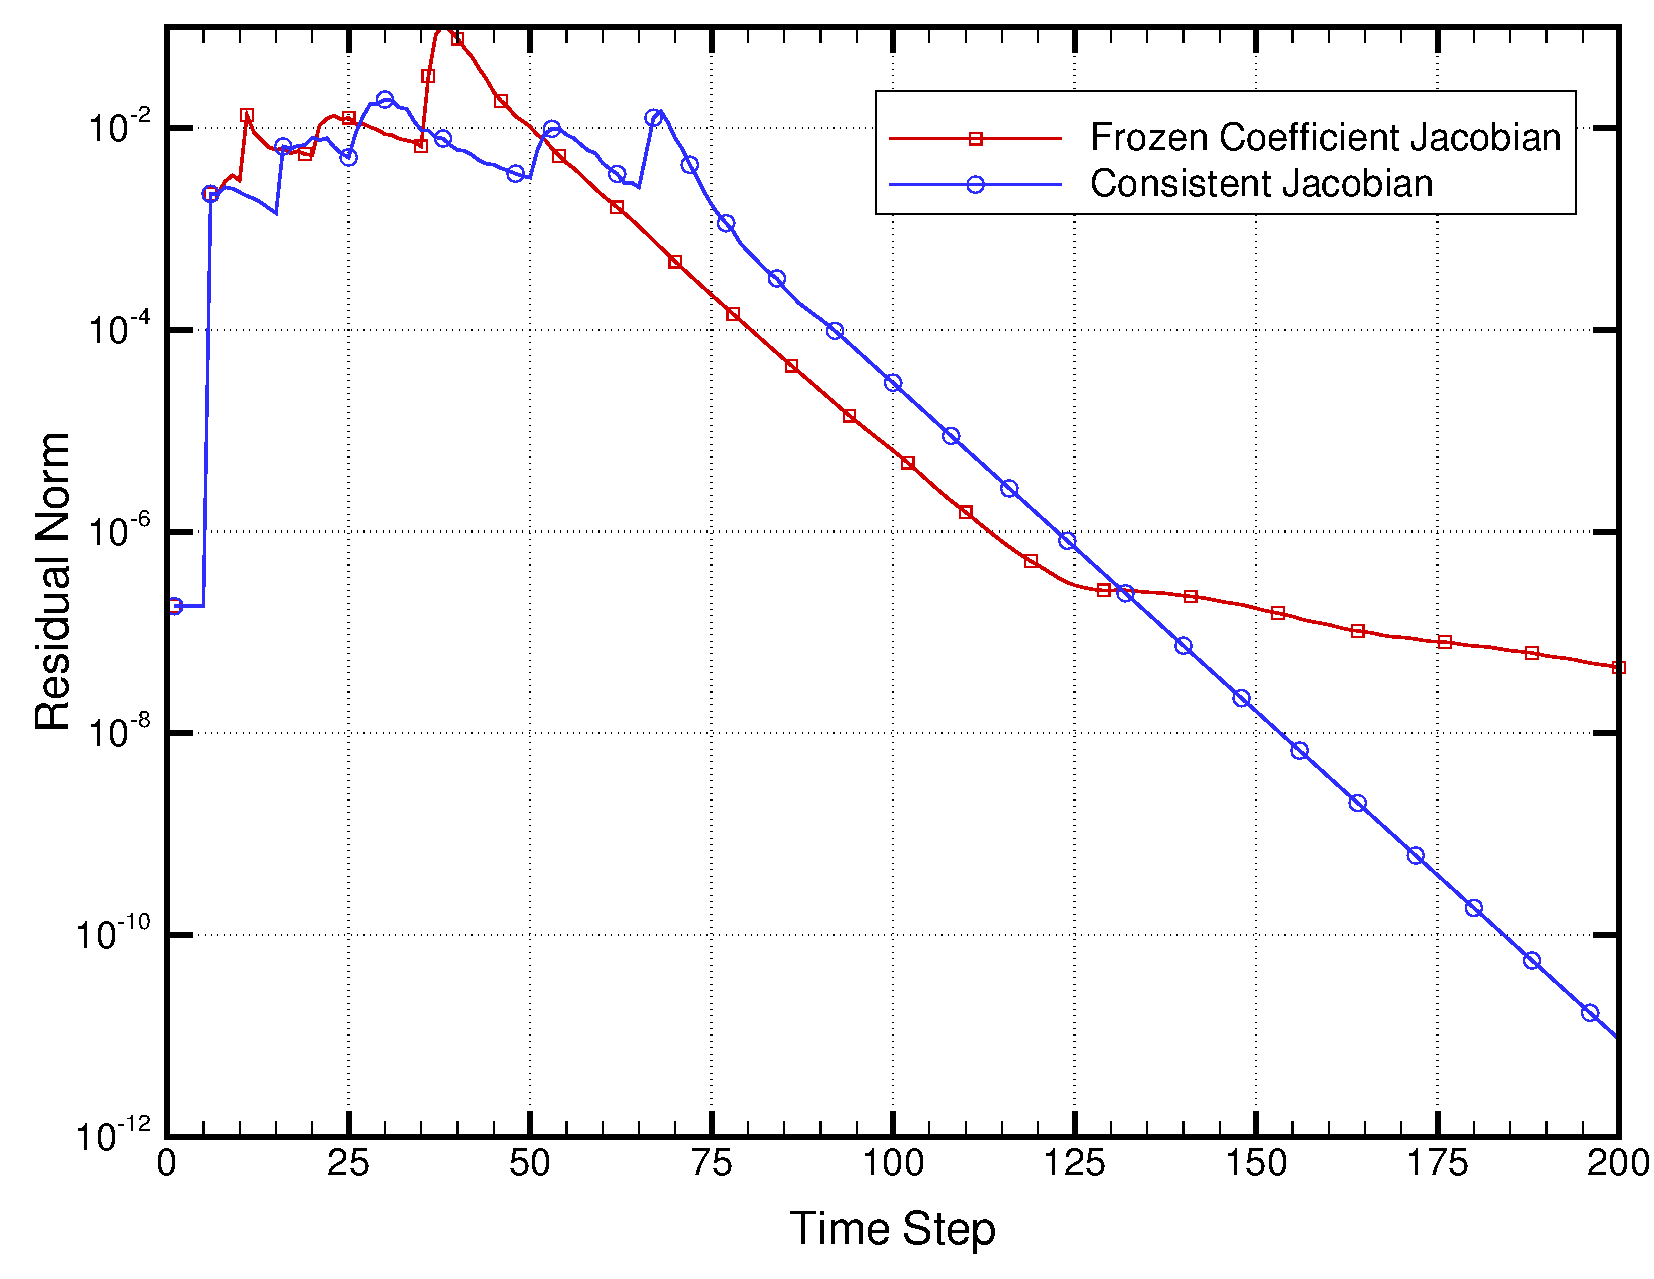
\includegraphics[width=\textwidth]{figures/convergence}

	Influence of linearization strategy on iterative convergence for Mach~3 flow over a cylinder
      \end{center}
    \end{block}
  \end{columns}
}

\section{Applications}
\frame
{
  \vspace{4em}
  \centerline{\huge{Hypersonic Aerothermodynamics -- }}
  \vspace{.5em}
  
  \centerline{\huge{ Application Studies}}
}


\subsection{Type~IV Shock Interaction}
\frame
{
  \frametitle{\scriptsize The X-15 Experience}
  \vspace{-1.5em}
  \begin{center}
    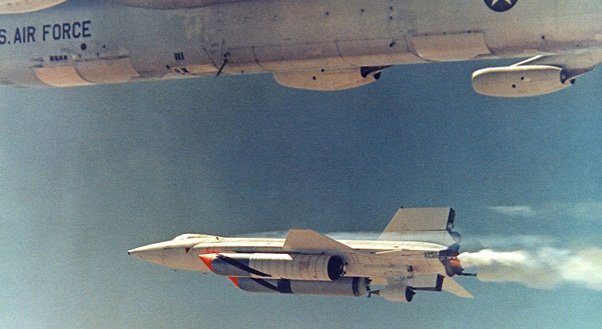
\includegraphics[width=.71\textwidth]{figures/x15/x15-25} \\

    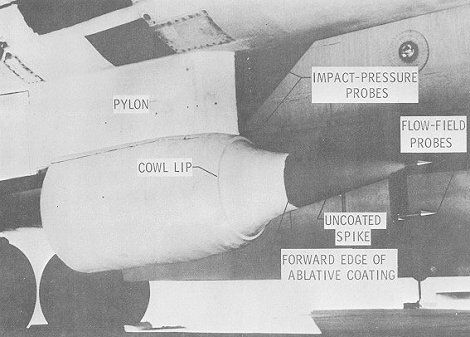
\includegraphics[height=.3\textheight]{figures/x15/x15-ramjet} \hspace{.5em}
    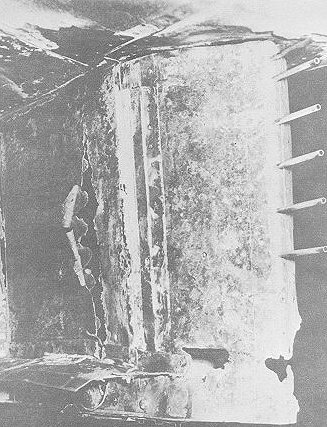
\includegraphics[height=.3\textheight]{figures/x15/x15-pylon} \hspace{.2em}
    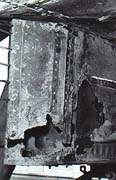
\includegraphics[height=.3\textheight]{figures/x15/x15-pylon2}
  \end{center}
}

\frame
{
  \frametitle{\scriptsize Edney's Type~IV Interaction Pattern~\cite{edney-ssi}}
  \vspace{-1.5em}
  \begin{center}
    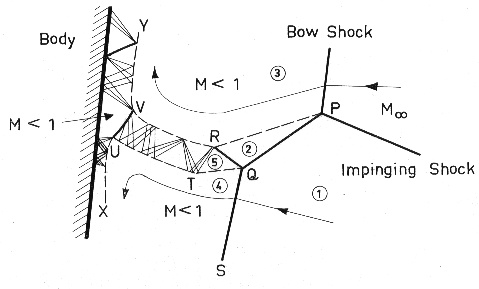
\includegraphics[width=.65\textwidth]{figures/edney/type4_schem}
    
    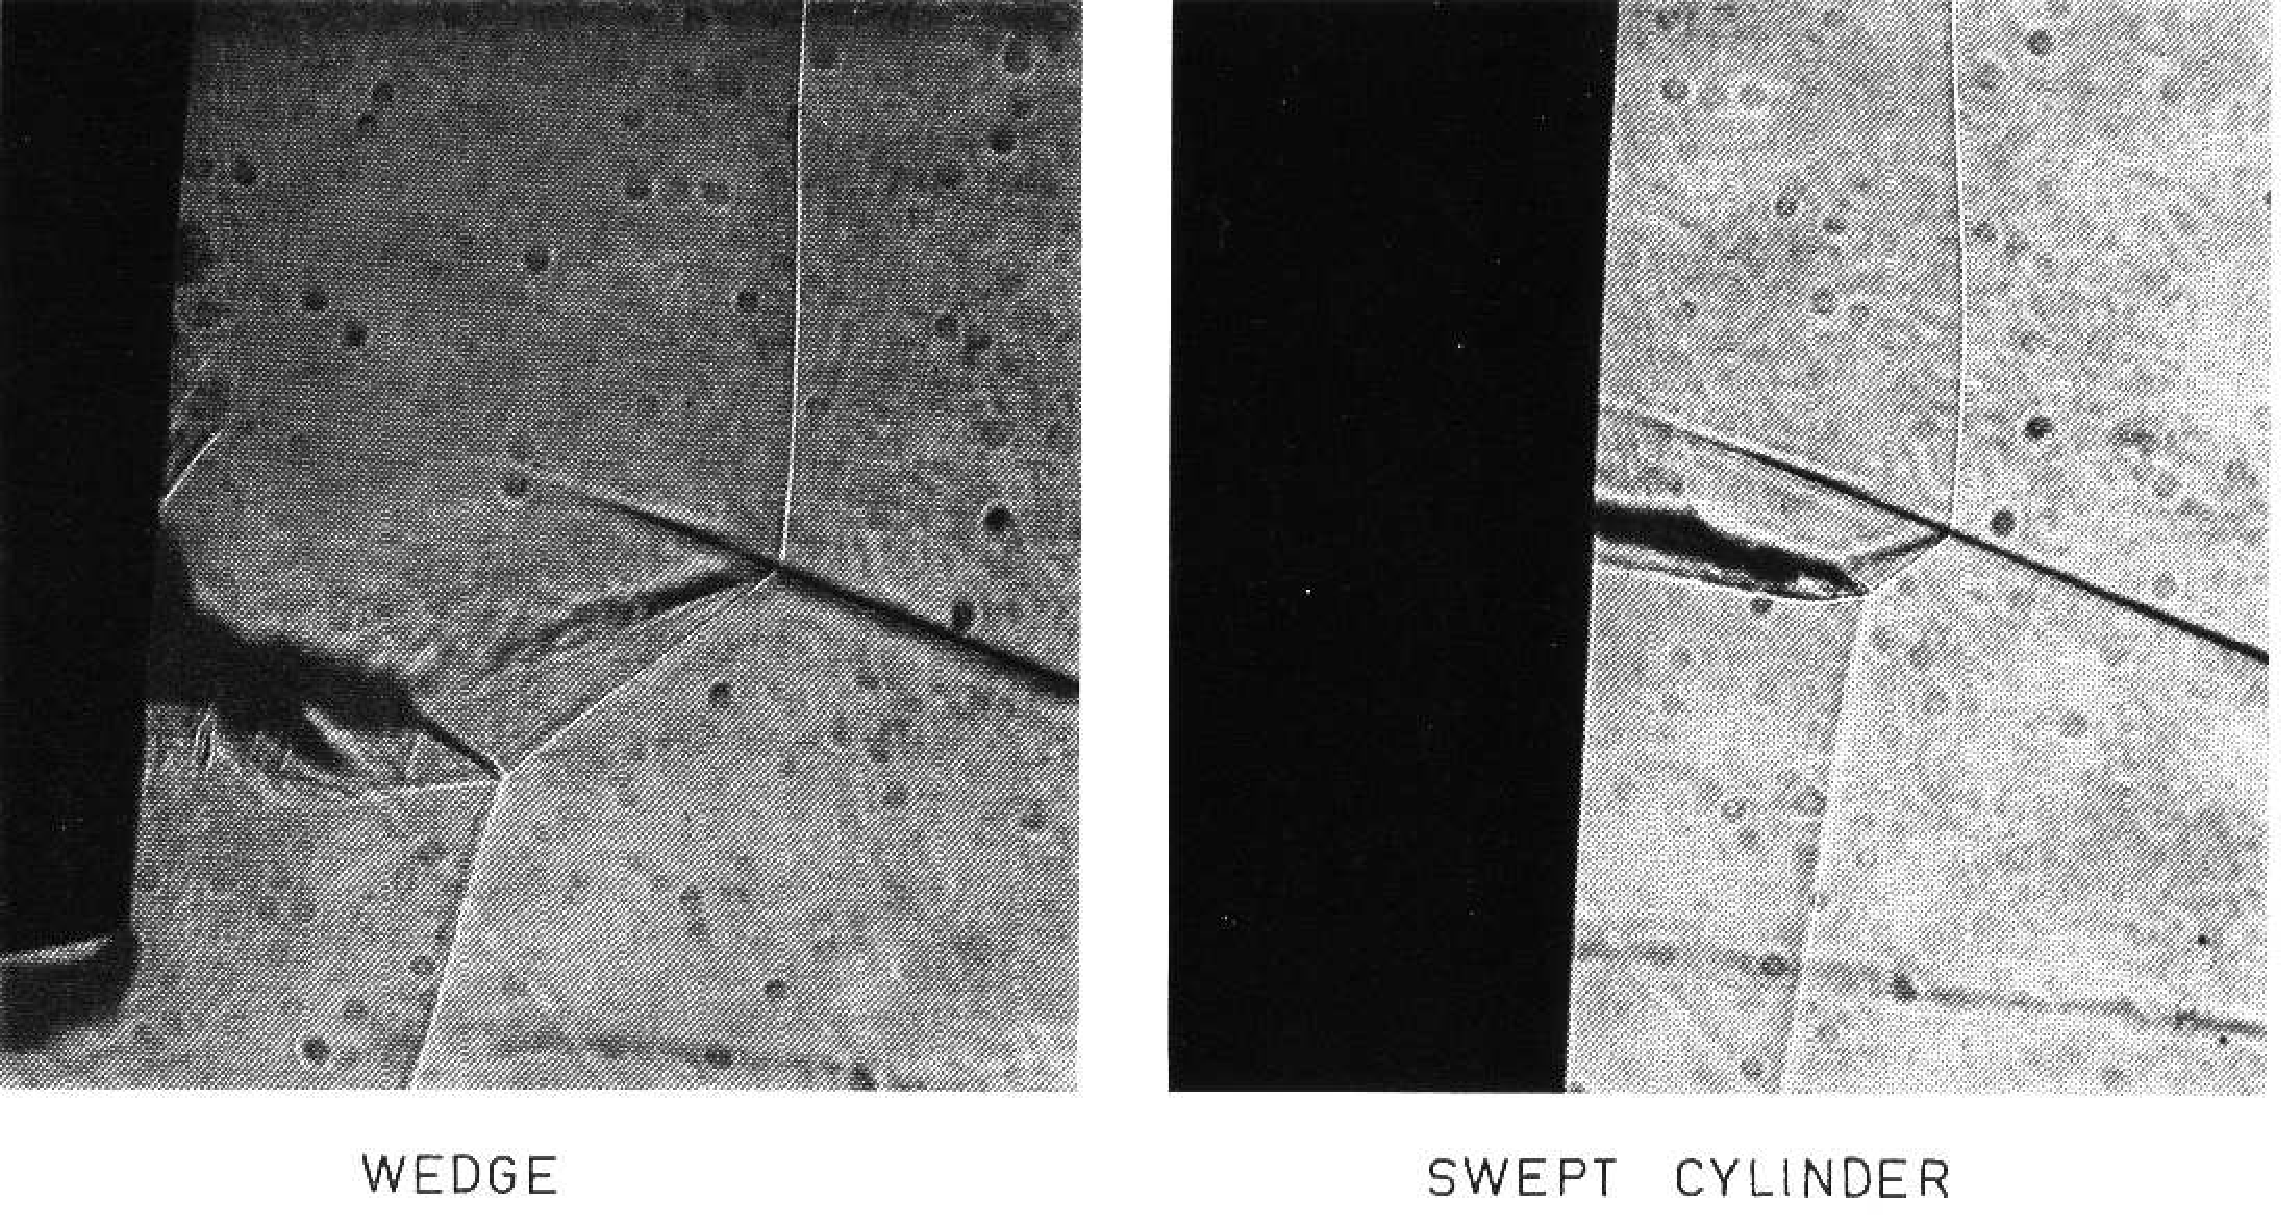
\includegraphics[width=.48\textwidth]{figures/edney/type4}
  \end{center}
}

\frame
{
  \scriptsize
 An experimental test program was conducted in 1998 by France's Office National d`Etudes et de Recherches A\'{e}rospatiales (ONERA) to investigate shock-shock interactions produced by an oblique shock impinging on the bow shock of a cylinder~\cite{onera-hypersonic-ssi}.  This configuration is examined here to assess the quality of surface heat transfer predictions.

 \begin{center}
    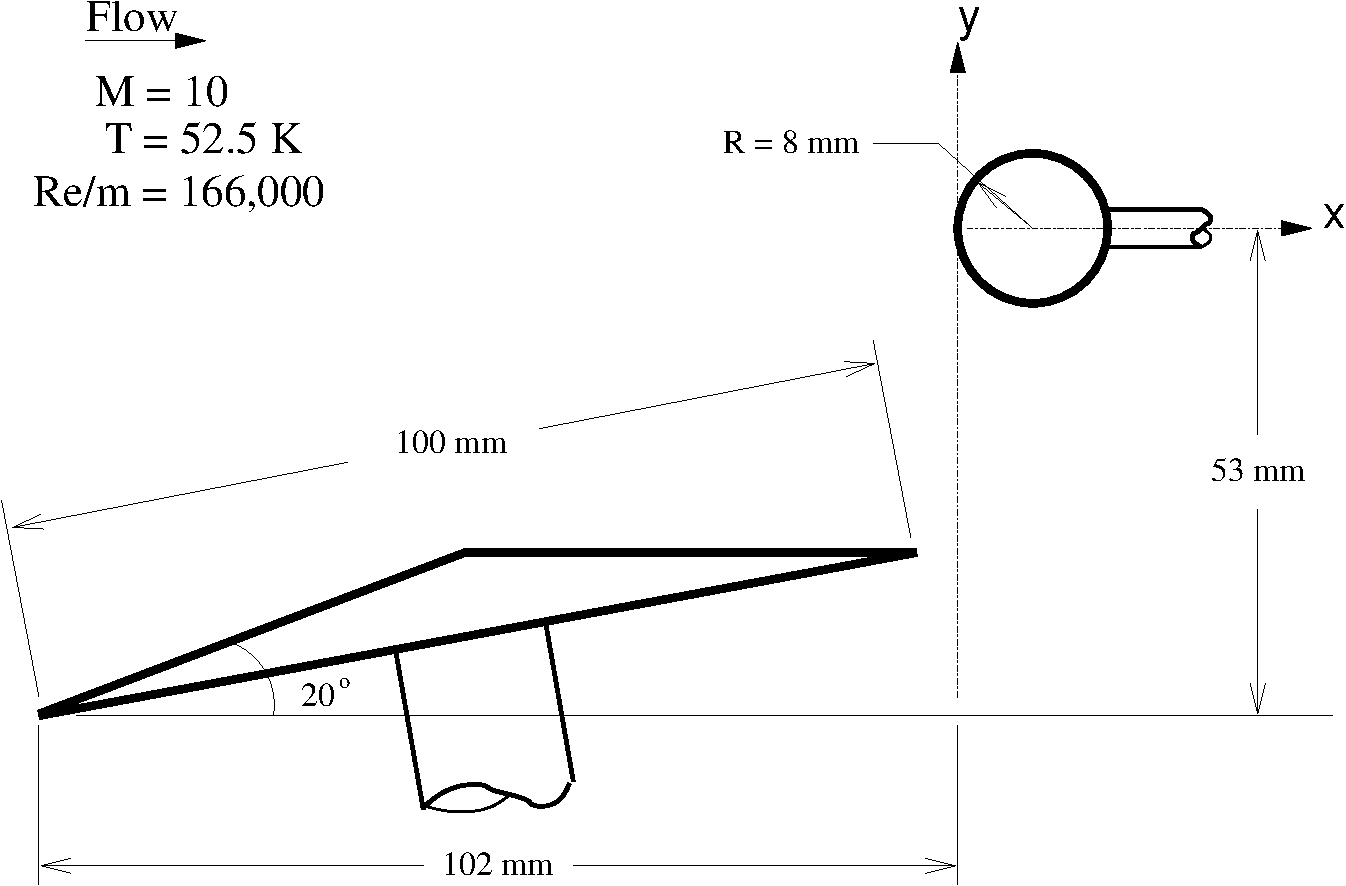
\includegraphics[width=.7\textwidth]{figures/onera_type4_ssi/schematic}
  \end{center}
}

\frame
{
  \begin{center}
    \scriptsize
    Static temperature contours
    
    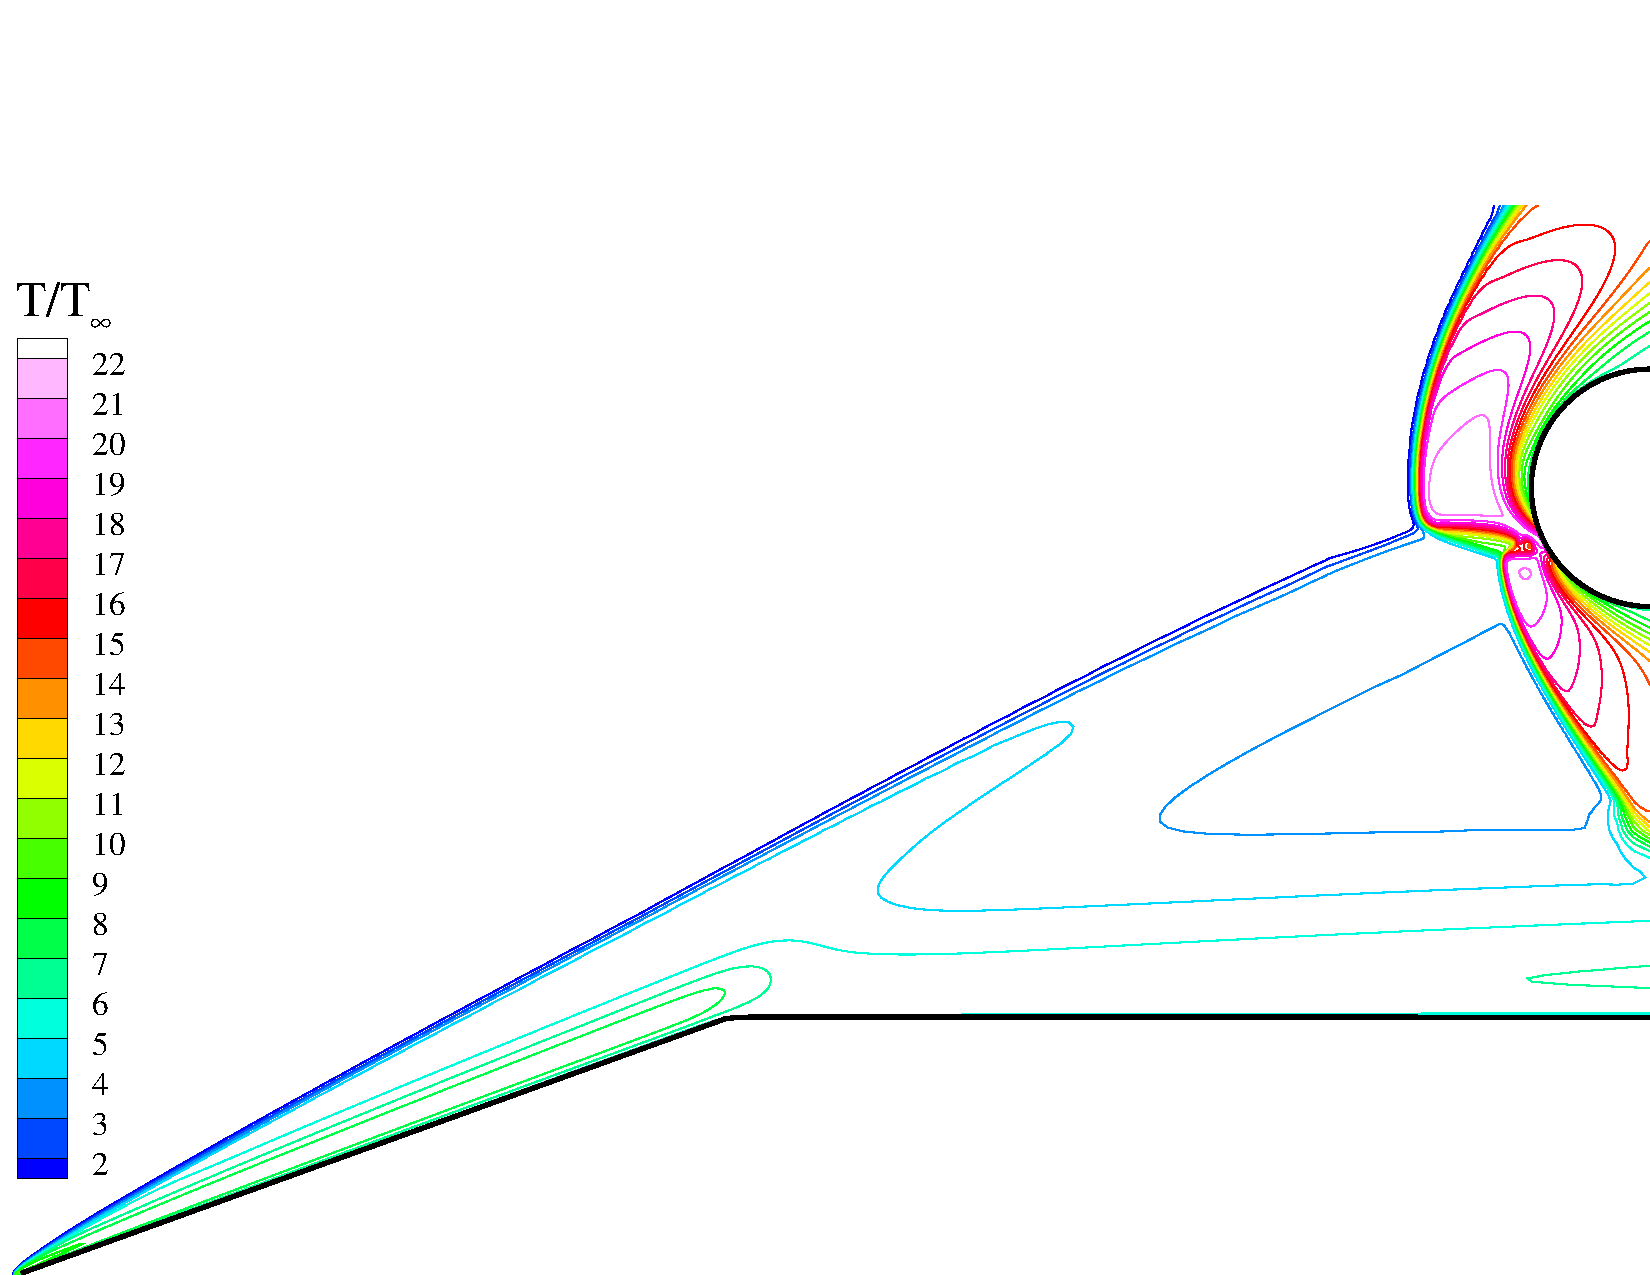
\includegraphics[width=.95\textwidth]{figures/onera_type4_ssi/T_global}
  \end{center}
}

\frame
{
  \begin{center}
    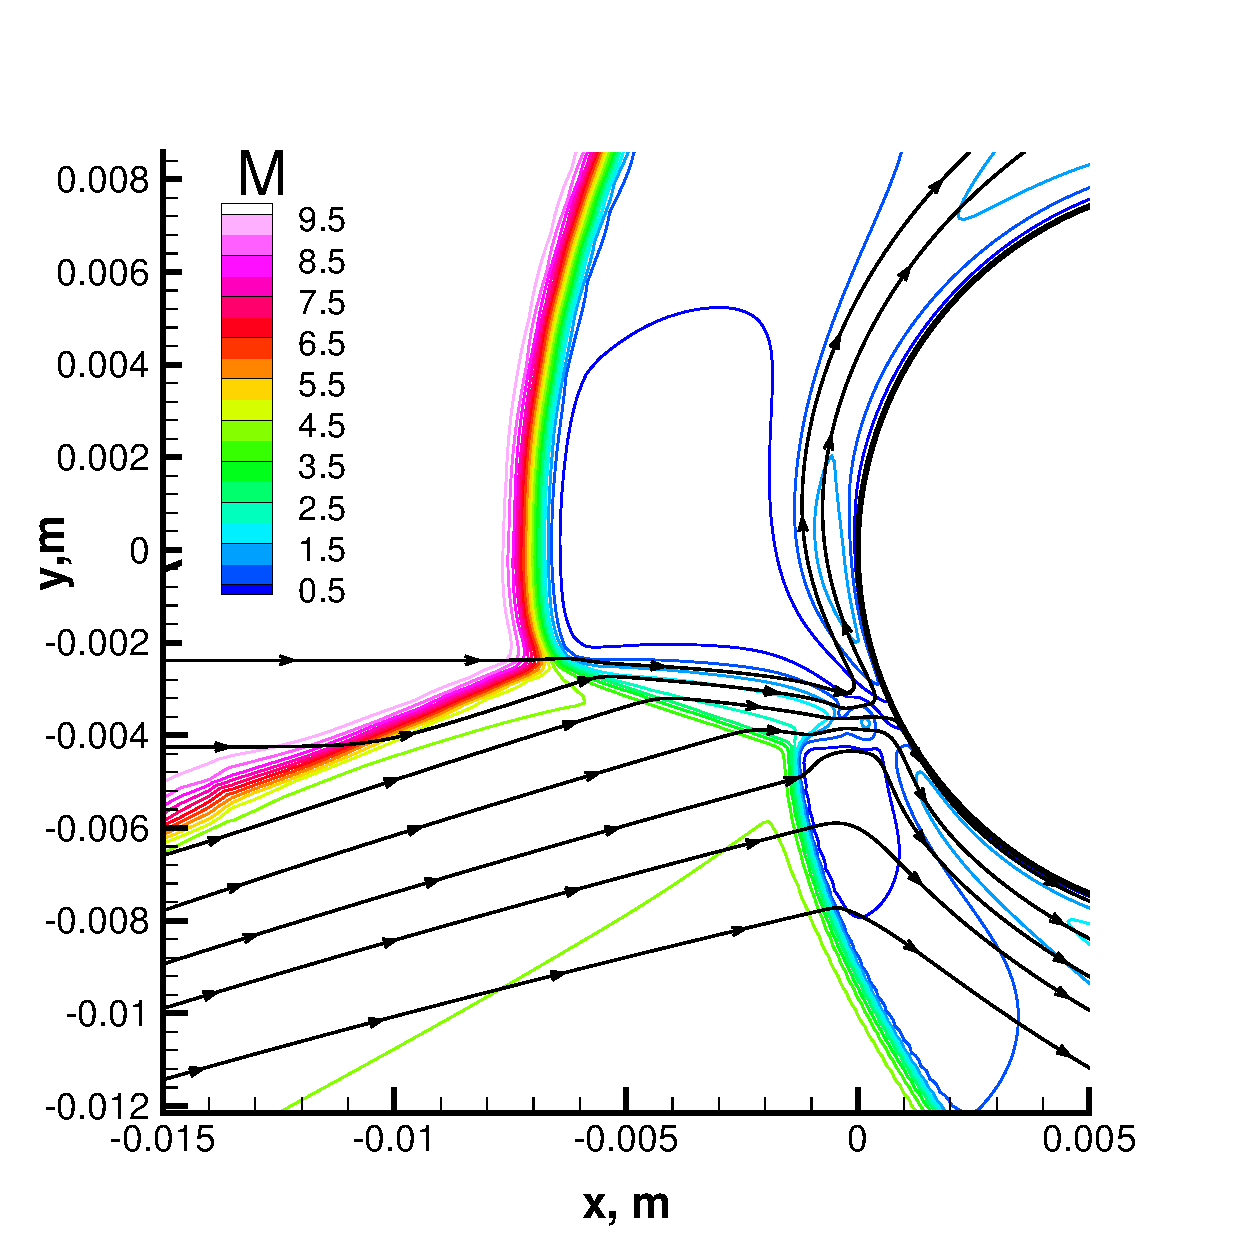
\includegraphics[width=.48\textwidth]{figures/onera_type4_ssi/M_local}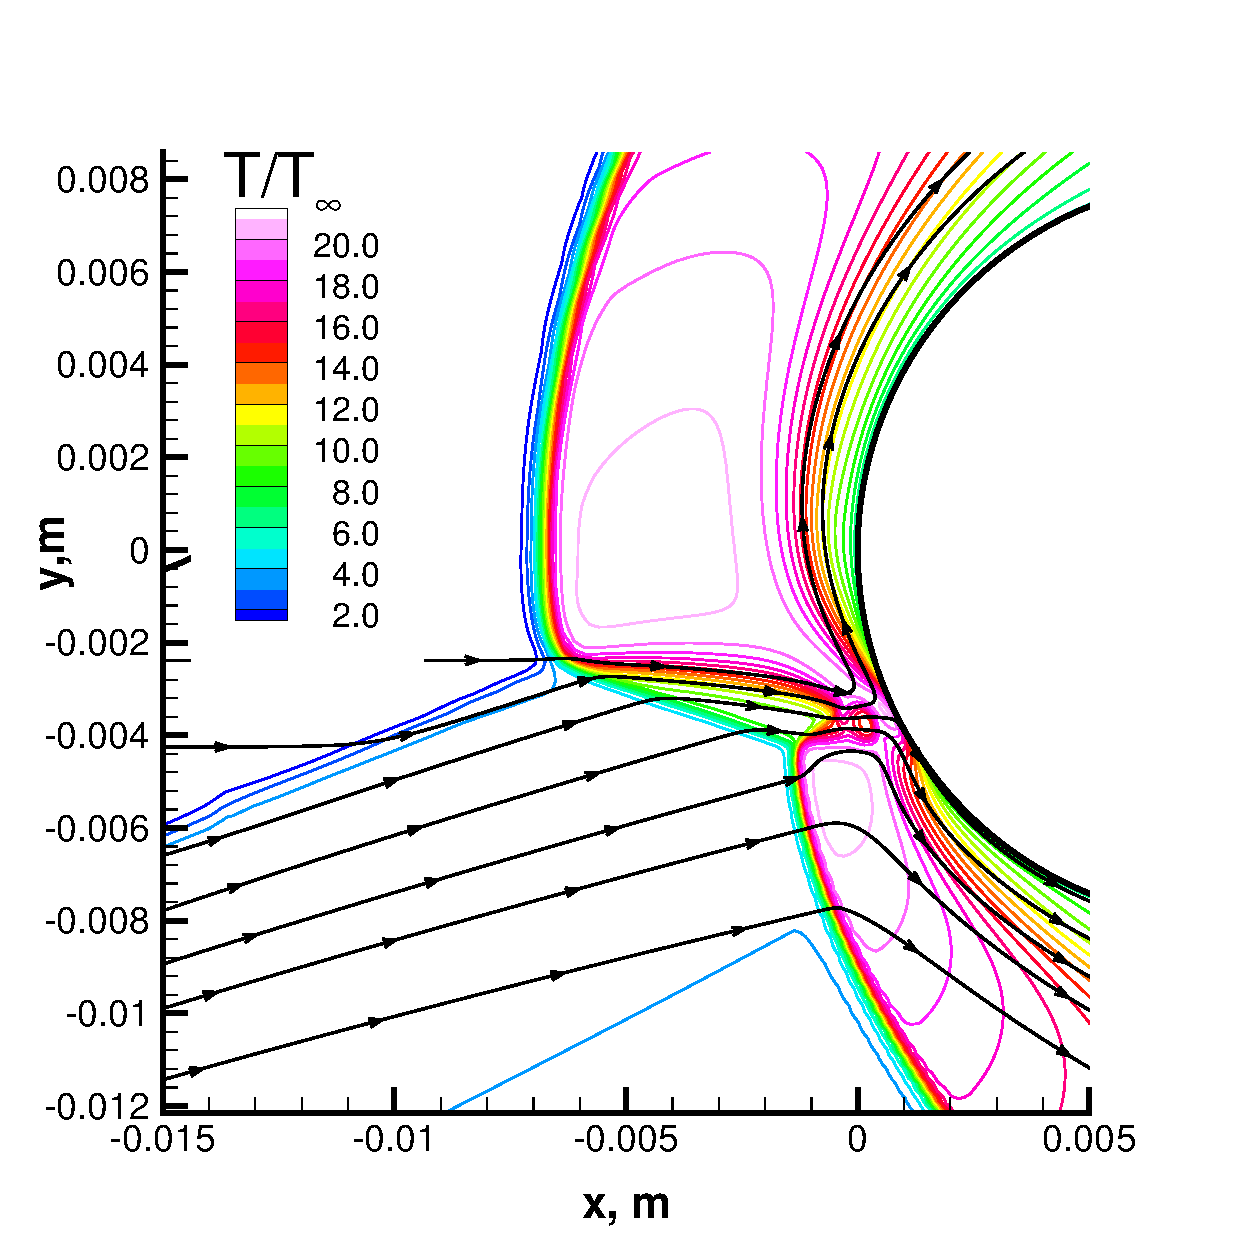
\includegraphics[width=.48\textwidth]{figures/onera_type4_ssi/T_local}
  \end{center}
}

\frame
{
  \begin{center}
    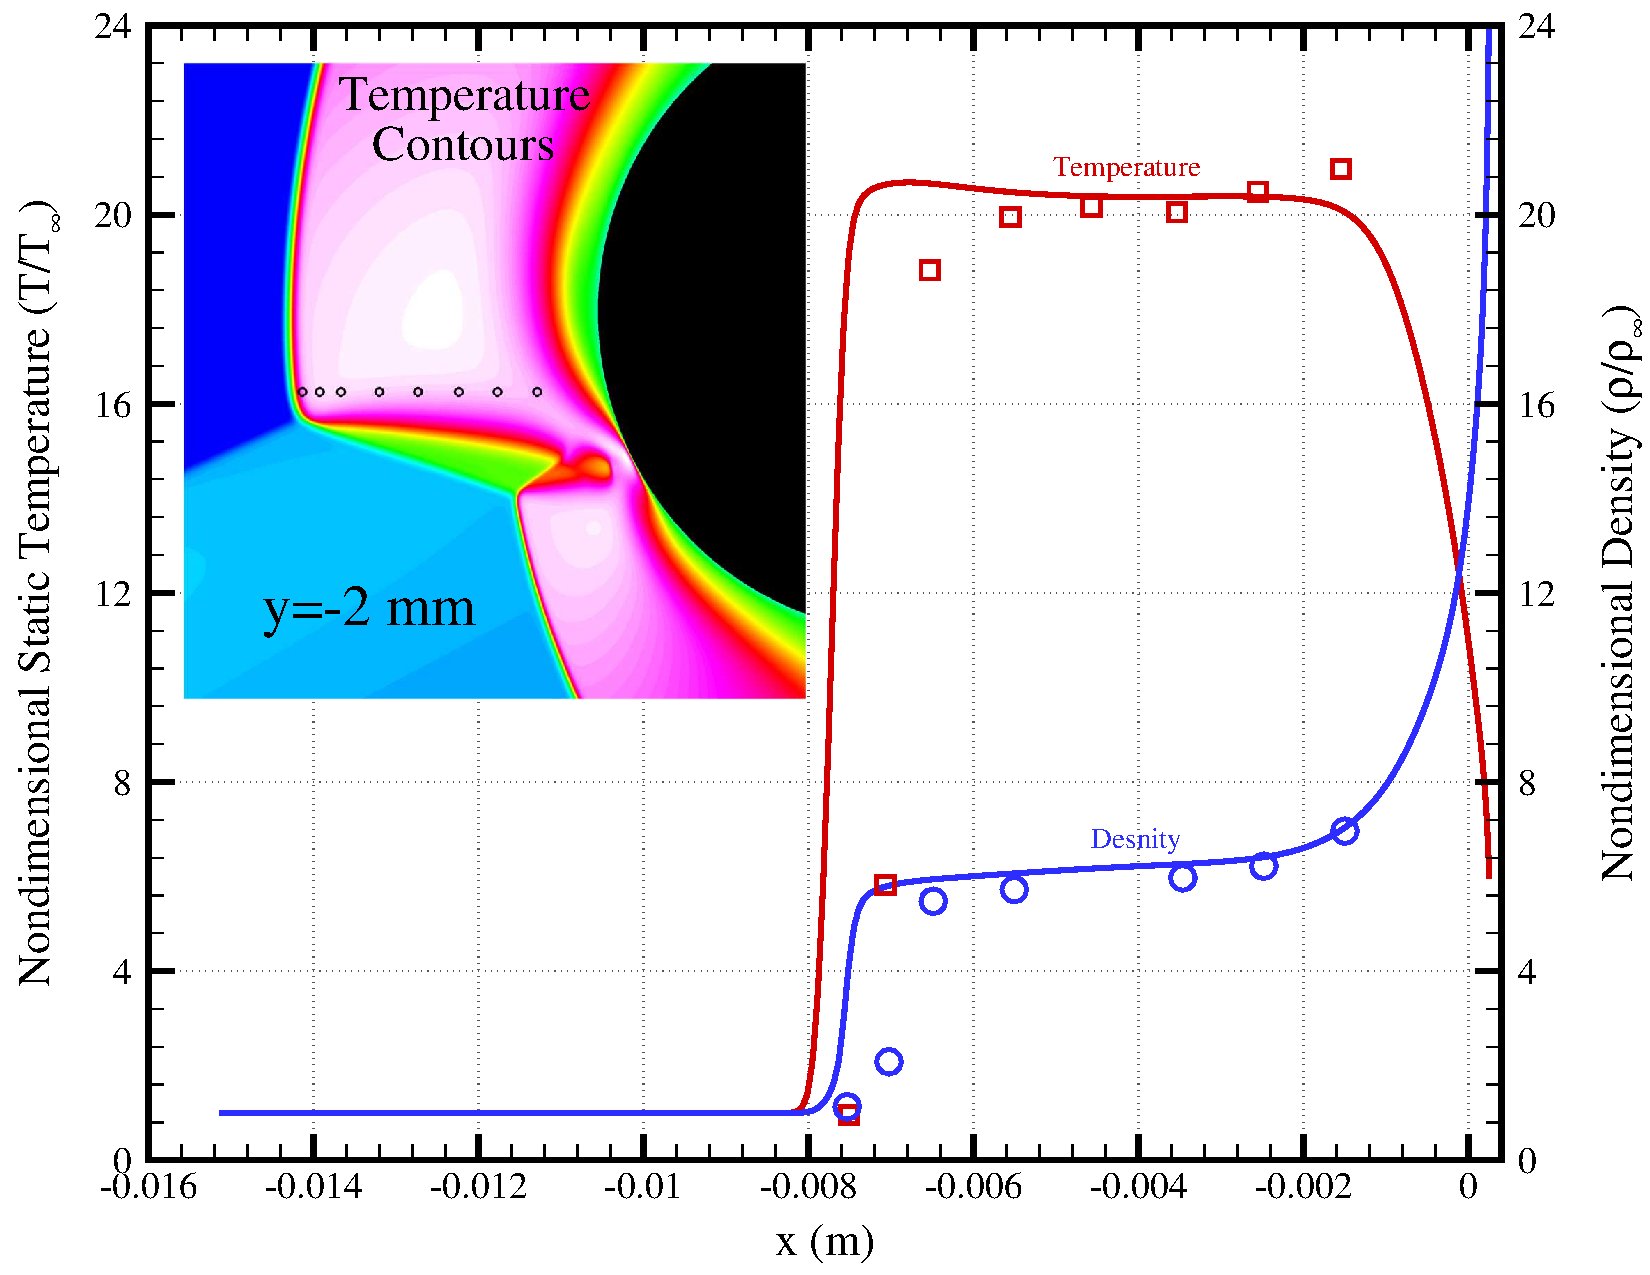
\includegraphics[width=.45\textwidth]{figures/onera_type4_ssi/y-2mm}\hspace{1em}
    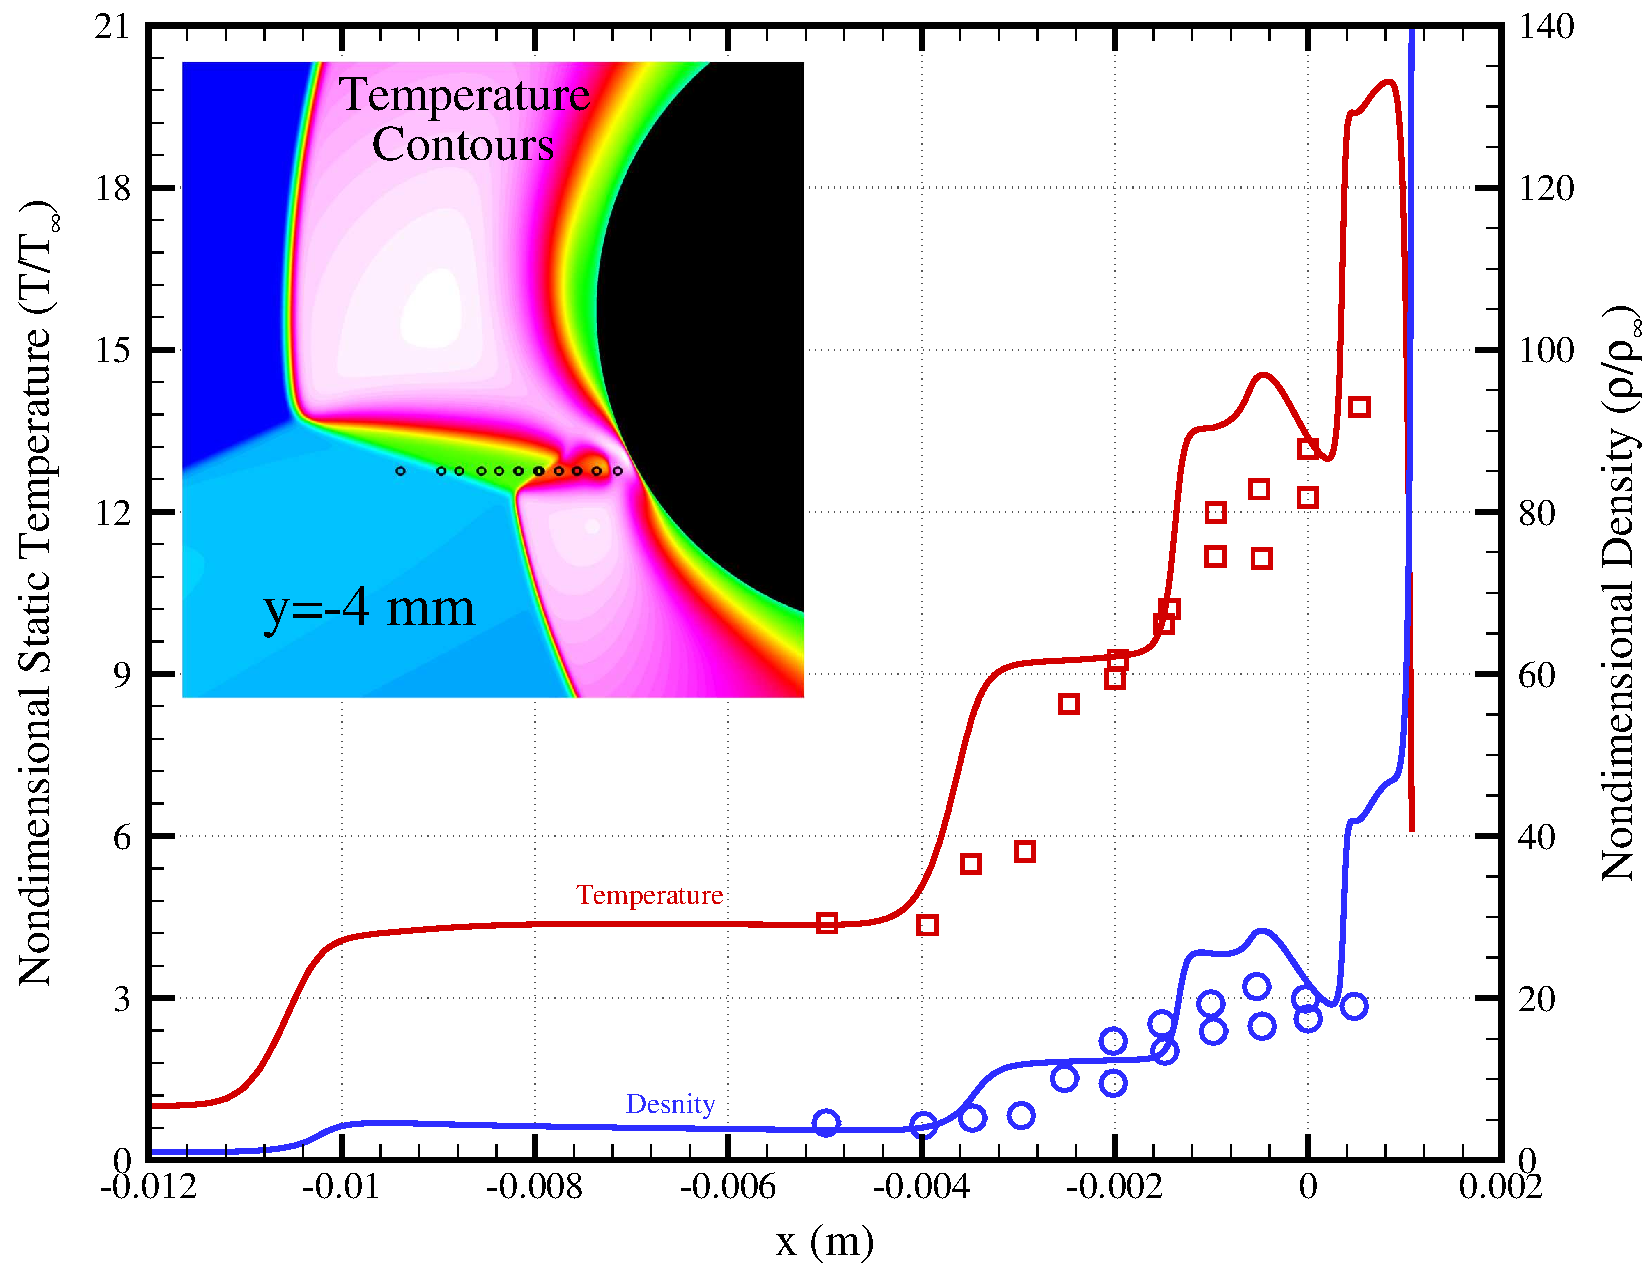
\includegraphics[width=.45\textwidth]{figures/onera_type4_ssi/y-4mm}
  
    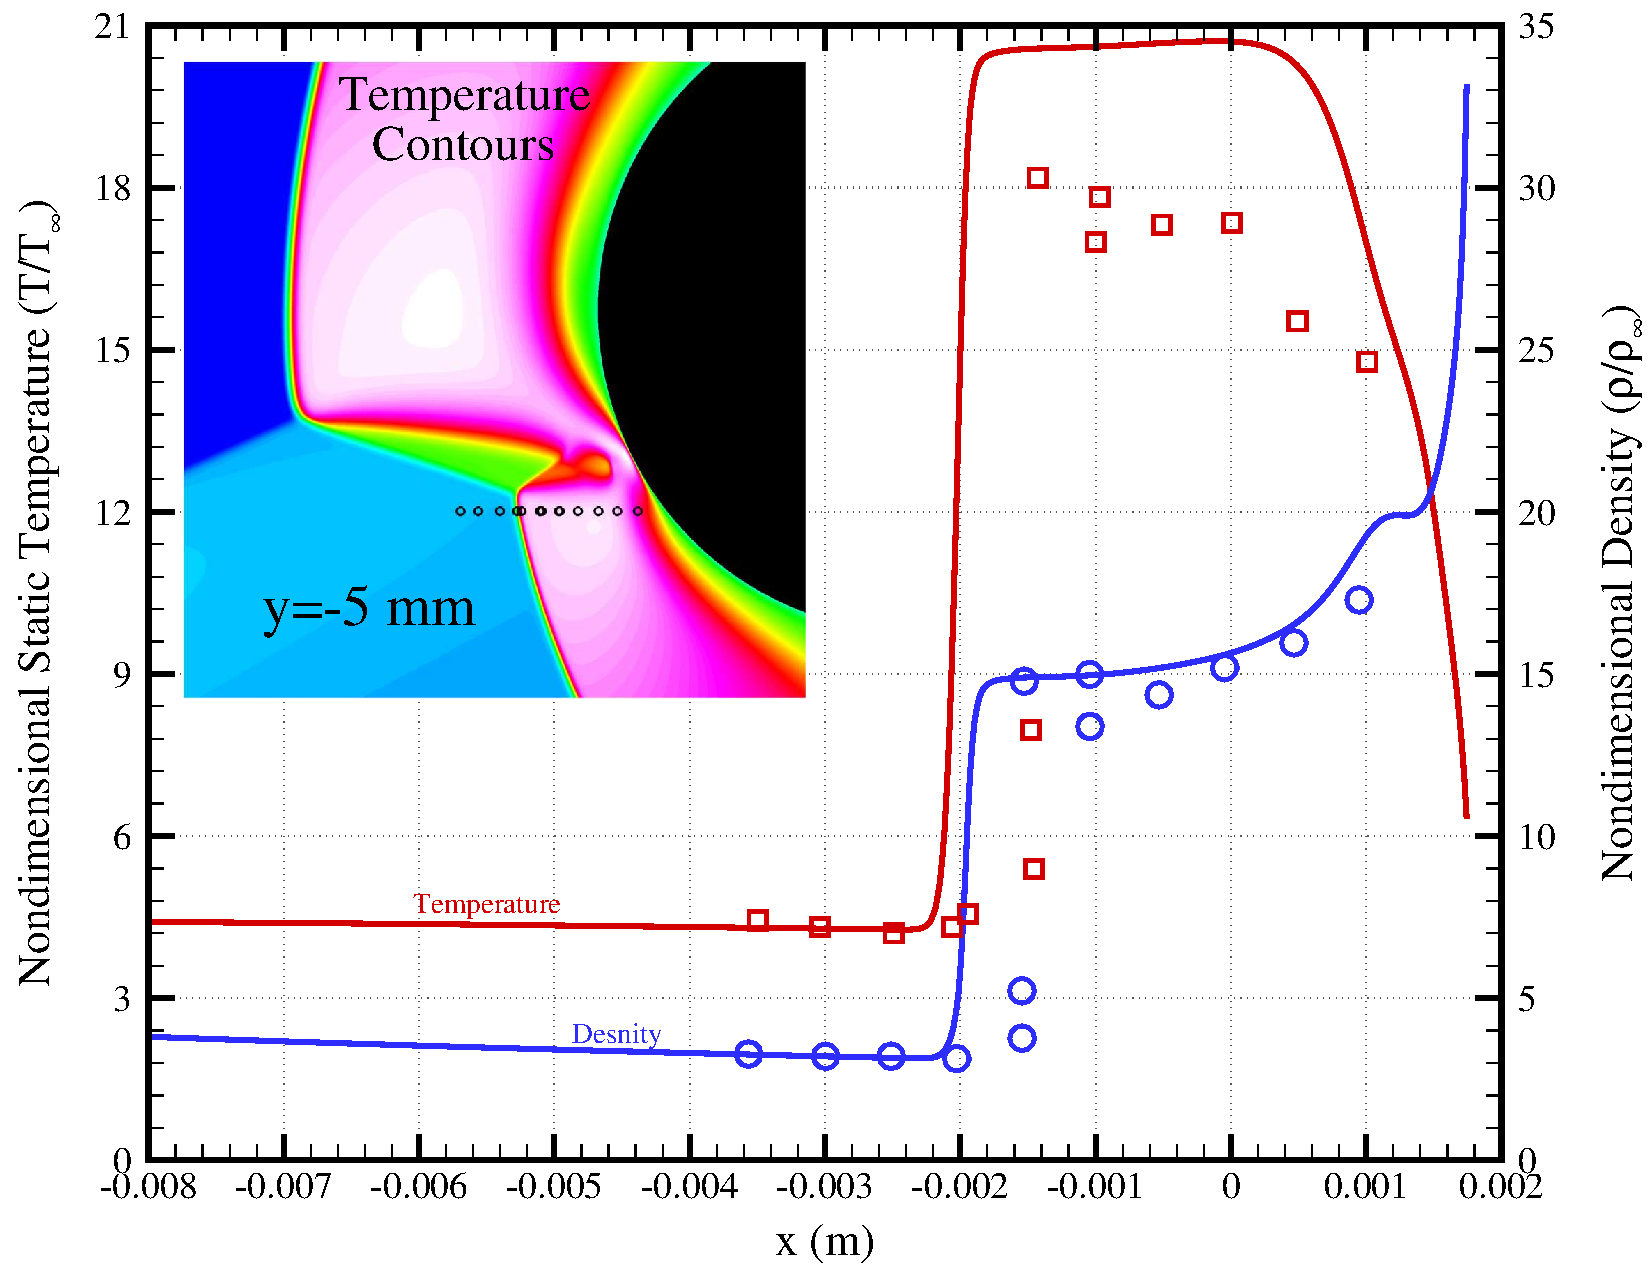
\includegraphics[width=.45\textwidth]{figures/onera_type4_ssi/y-5mm}
  \end{center}
}

\frame
{
  \centerline{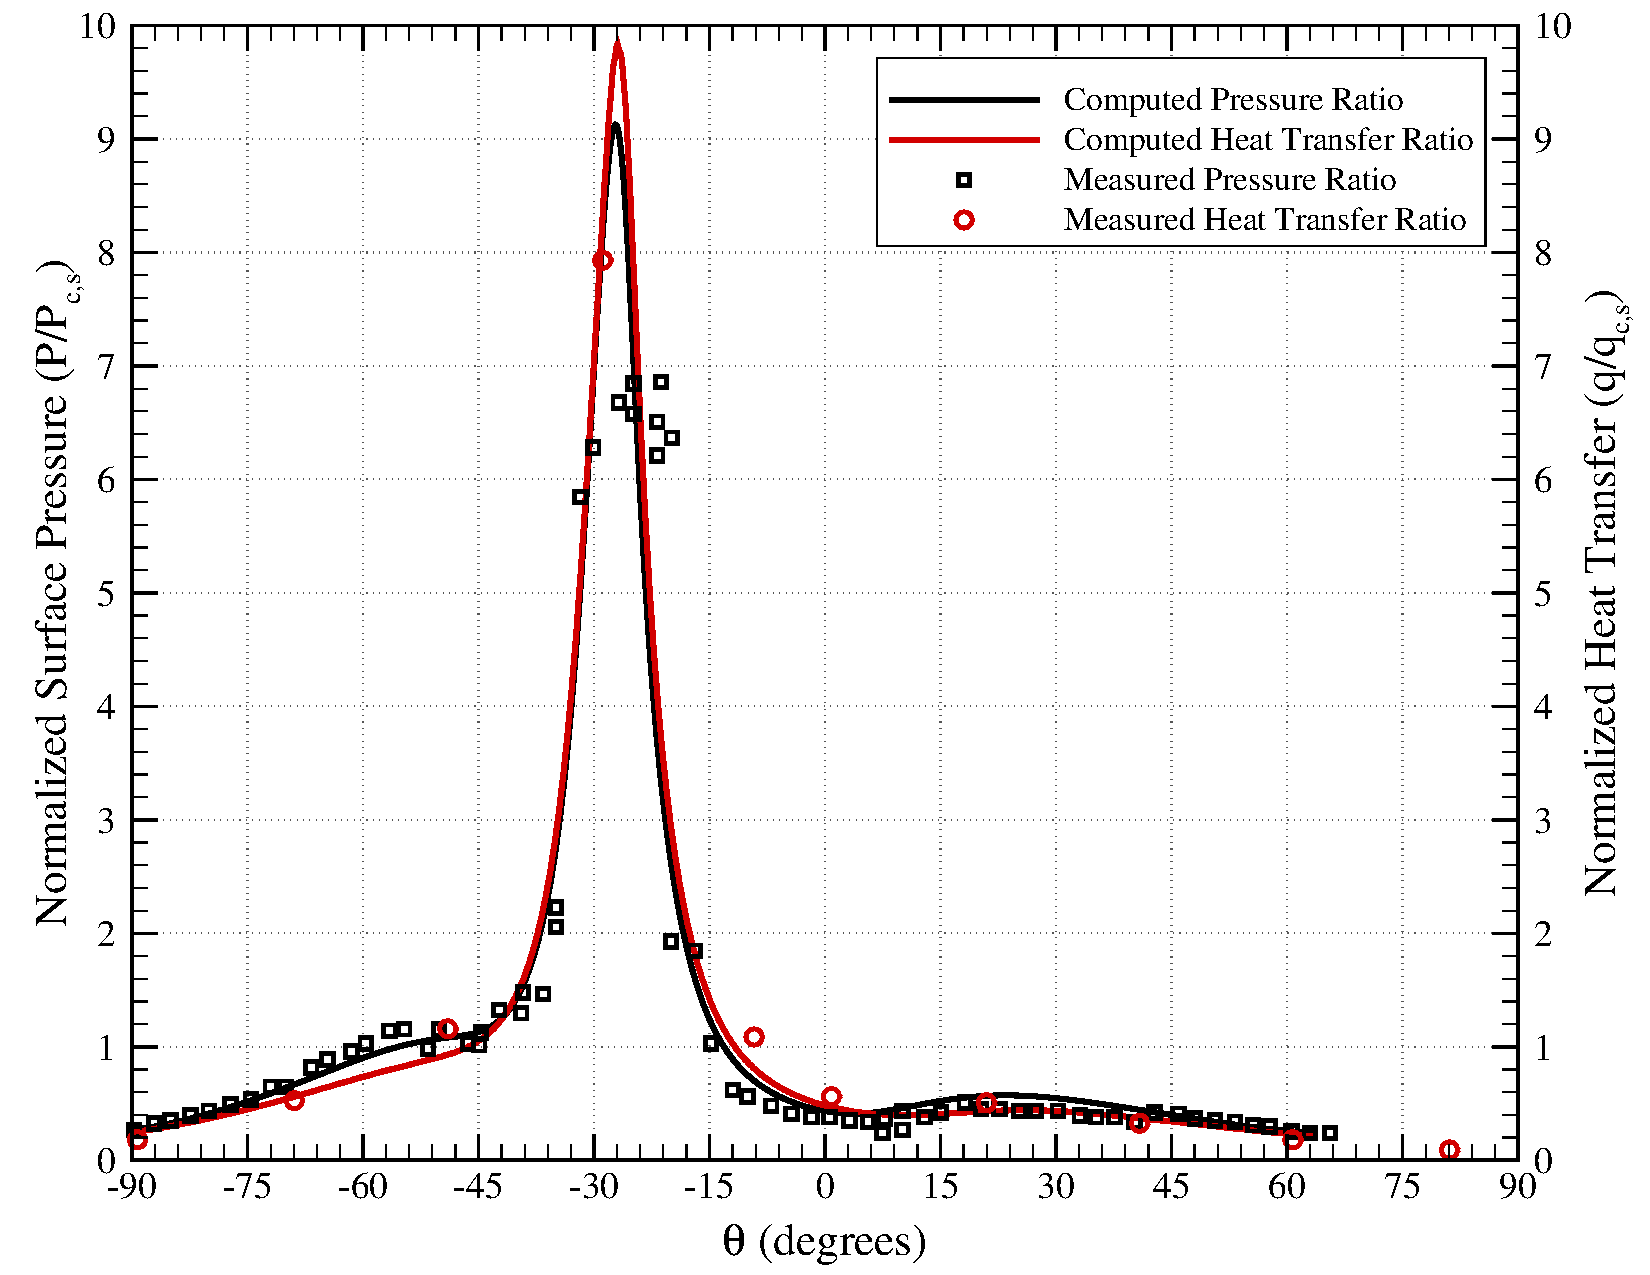
\includegraphics[width=.9\textwidth]{figures/onera_type4_ssi/p_q_ratios}}
}

%% \frame
%% {
%%   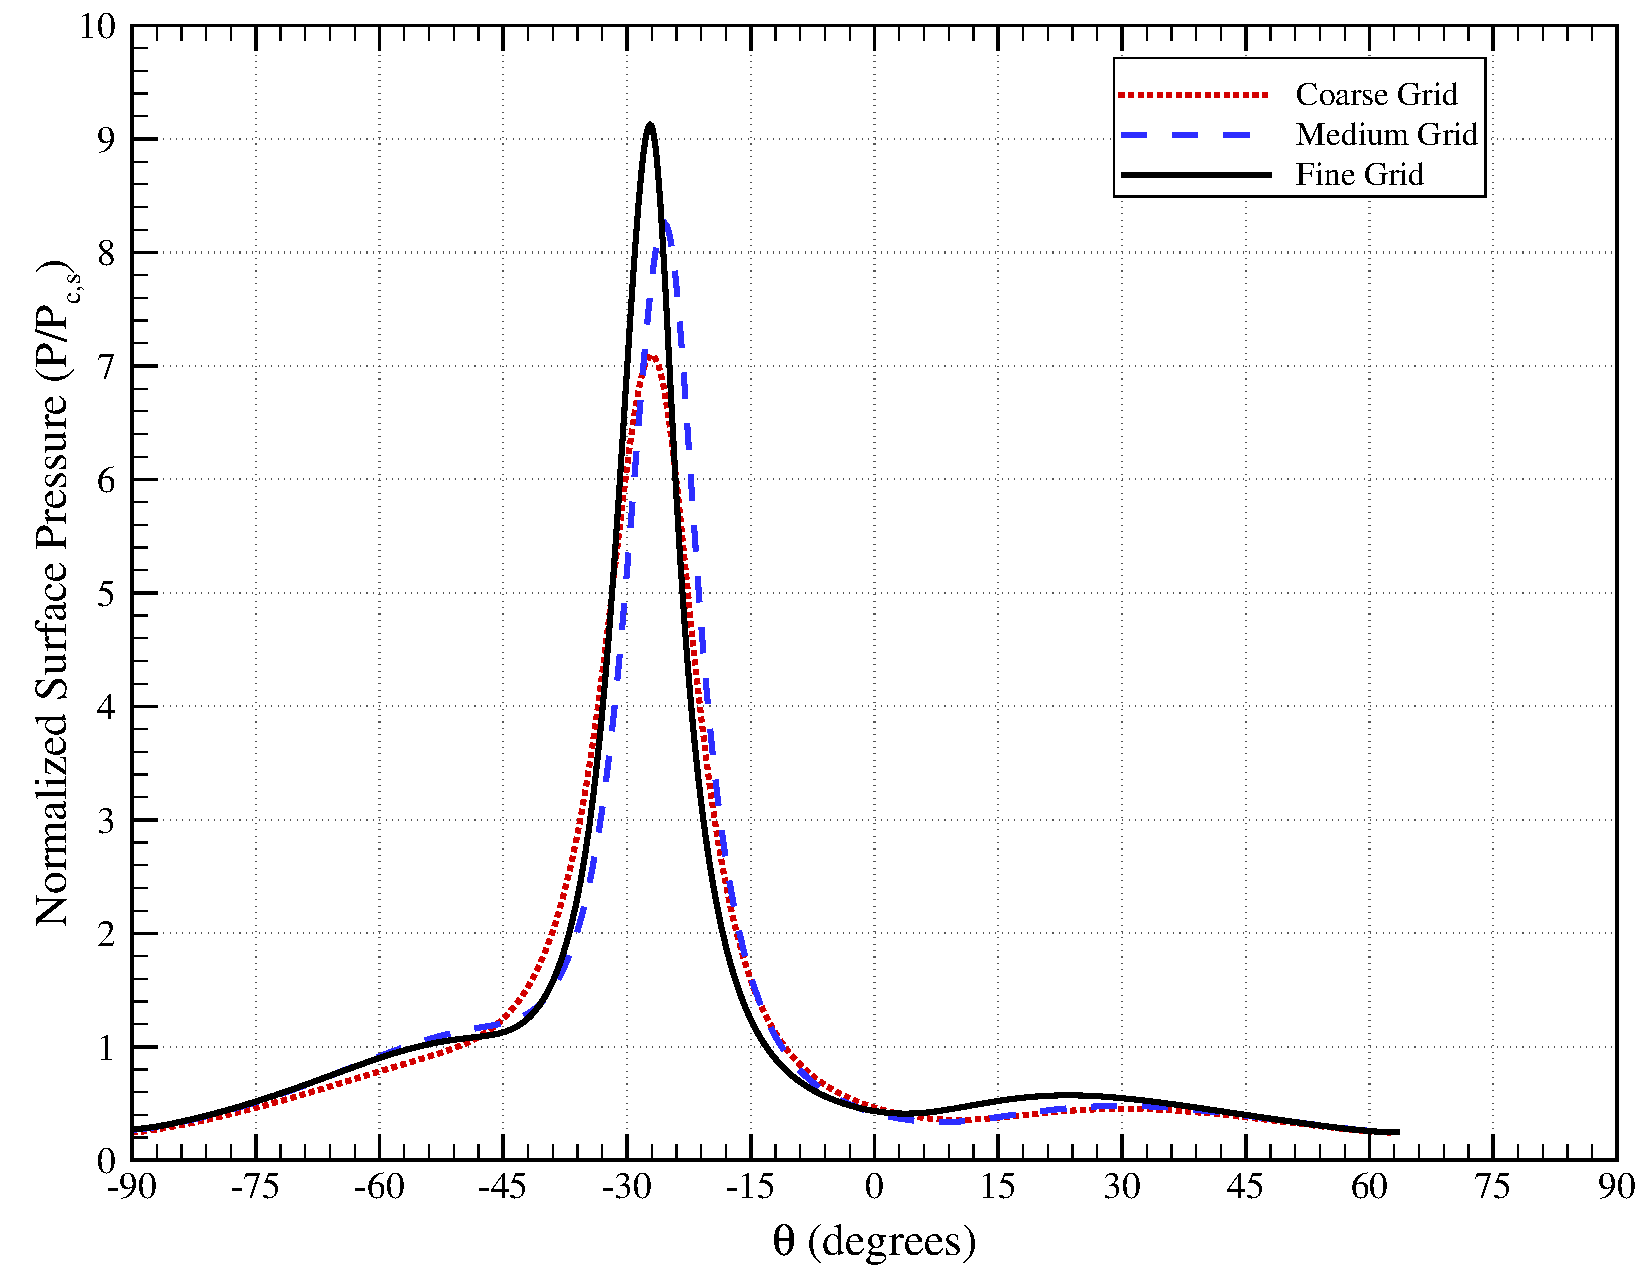
\includegraphics[width=.48\textwidth]{figures/onera_type4_ssi/pressure_convergence}
%%   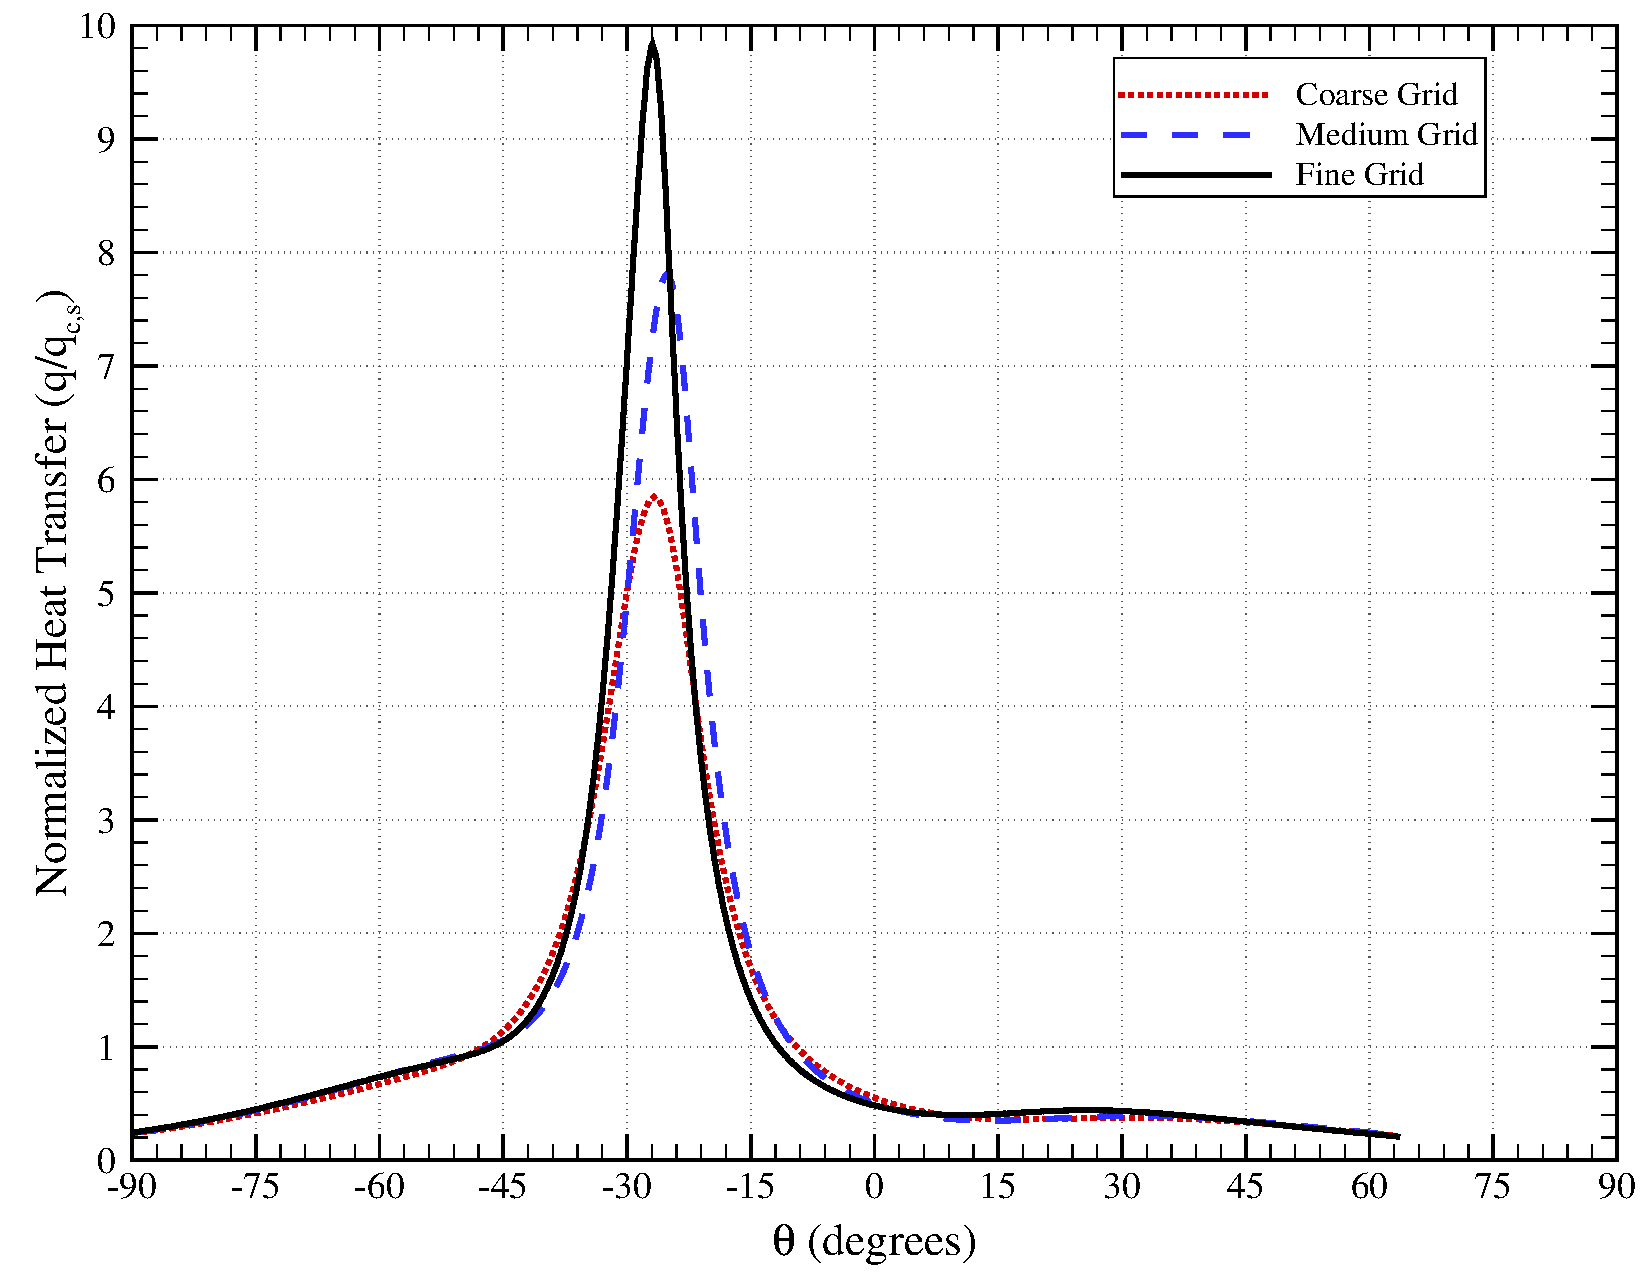
\includegraphics[width=.48\textwidth]{figures/onera_type4_ssi/heat_transfer_convergence}
%% }

\subsection{Forward-Facing Cavity}
\frame
{
  \scriptsize
  Hypersonic flow over a missile nose tip with a forward facing cavity has been observed to exhibit transient flowfield response in both experimental investigations and numerical simulations~\cite{engblom_goldstein_AIAA-1996-354,silton_goldstein_JTHPHT}. The flowfield response characteristics are largely driven by the cavity length-to-diameter ratio (L/D).  
  \begin{center}
    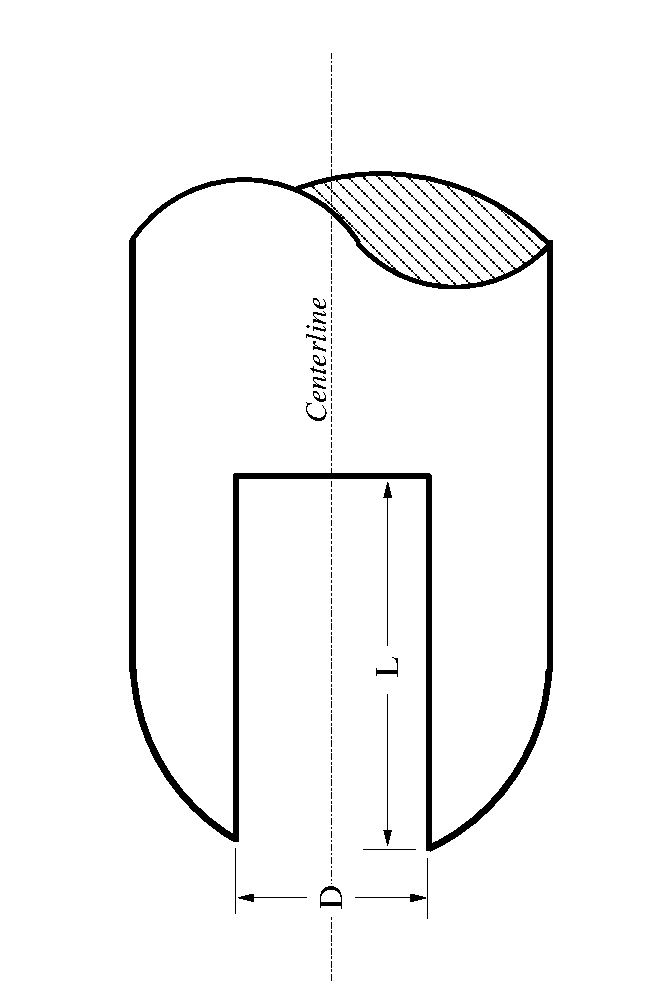
\includegraphics[angle=270,width=0.5\textwidth]{figures/sphere_cavity/LD_2.0/schematic}
  \end{center}
  
  Experimental studies in conventional tunnels report oscillatory response even for relatively shallow cavities, suggesting a threshold L/D of 0.4. Numerical simulations predict a higher threshold L/D of $\approx 1.25$.  Subsequent studies in a quiet wind tunnel verify the computational results, indicating freestream noise is the mechanism for driving unsteady response in shallow cavities~\cite{engblom_goldstein_AIAA-1996-667}.
}

\frame
{
  \centerline{\includemovie[autoplay,loop,text={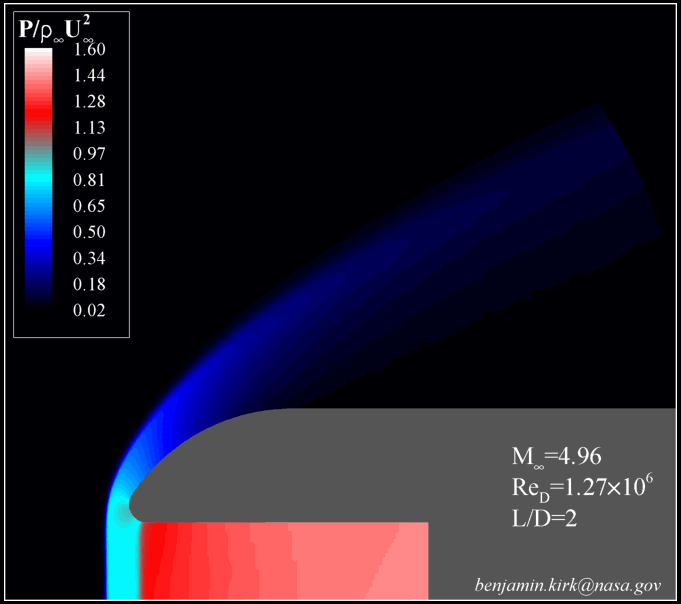
\includegraphics[height=.78\textheight]{figures/sphere_cavity/LD_2.0/P}}]{.8\textwidth}{.8\textheight}{movies/P_small.avi}}  
}

\frame
{
  \centerline{\includemovie[autoplay,loop,text={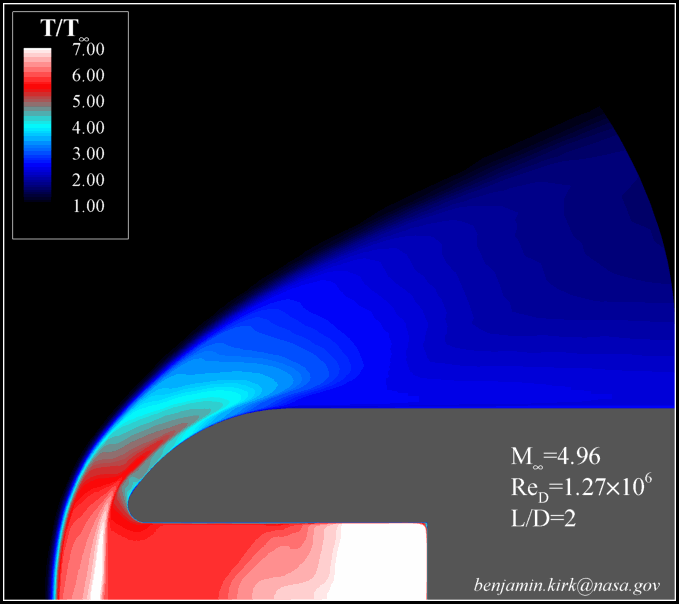
\includegraphics[height=.78\textheight]{figures/sphere_cavity/LD_2.0/T}}]{.8\textwidth}{.8\textheight}{movies/T_small.avi}}  
}

\frame
{
  \vspace{-.5em}
  \scriptsize
  Cavity base pressure versus time for a series of simulations used to assess time convergence.

  For CFL$_{\text{max}}=20\times 10^3$ there are $\approx 200$ time steps per oscillation cycle.
  \vspace{.5em}

  \centerline{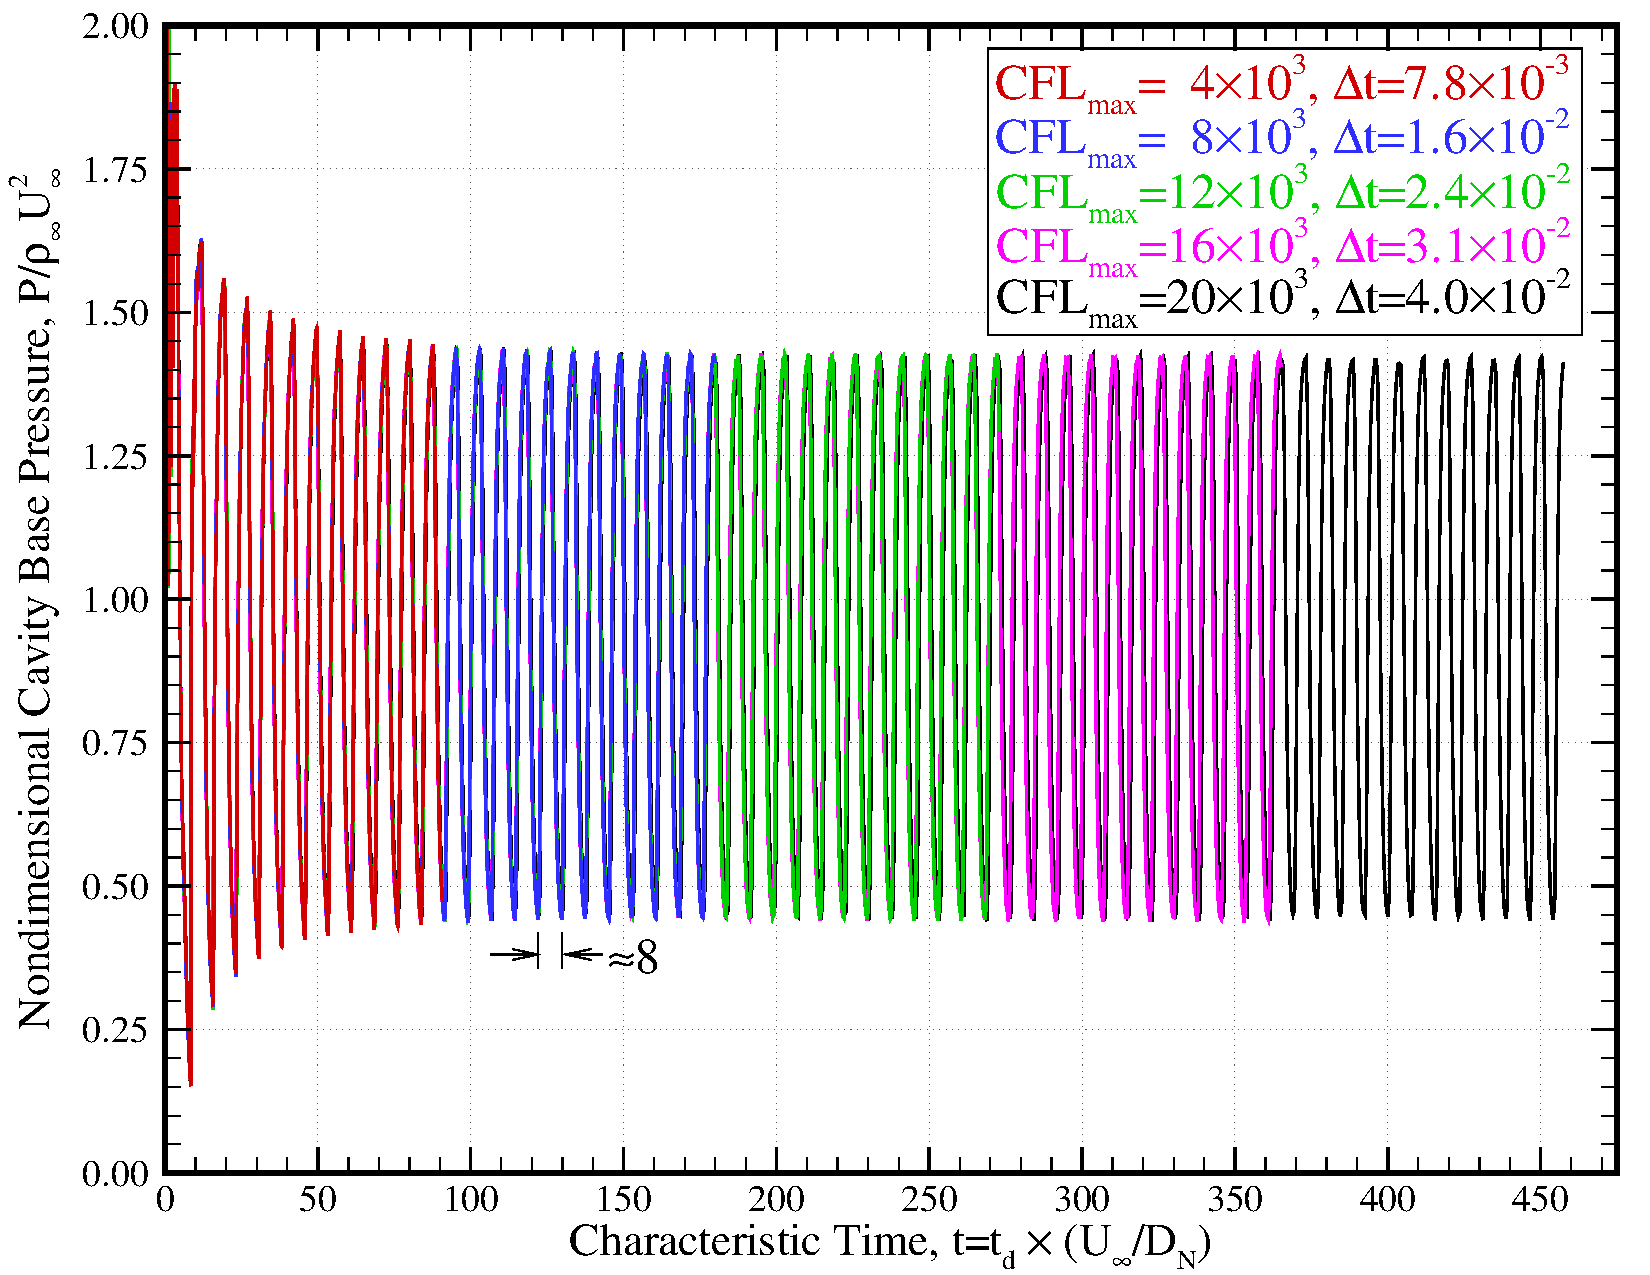
\includegraphics[width=0.85\textwidth]{figures/sphere_cavity/LD_2.0/base_pressure_history}}
}

\subsection{AEDC Sharp Double Cone}
\frame
{
  \begin{columns}[t]
    \column{.5\textwidth}
    \vspace{-1em}
    \begin{block}{Background}
      \footnotesize
      \begin{itemize}
        \item A sharp 25$^\circ$--55$^\circ$ double cone was tested in N$_2$ at CUBRC
	\item It was discovered that freestream vibrational nonequilibrium must be properly modeled for CFD to match experiment~\cite{nompelis_candler_holden_double_cone}
	\item The AEDC Hypervelocity Wind Tunnel No.~9 also uses N$_2$ as its test gas
	\item A series of tests were conducted at AEDC using the same model to investigate the presence of vibrational nonequilibrium in the freestream~\cite{AEDC_HVWT9_double_cone}
      \end{itemize}
    \end{block}
    
    \column{.5\textwidth}
    \vspace{2em}
    
    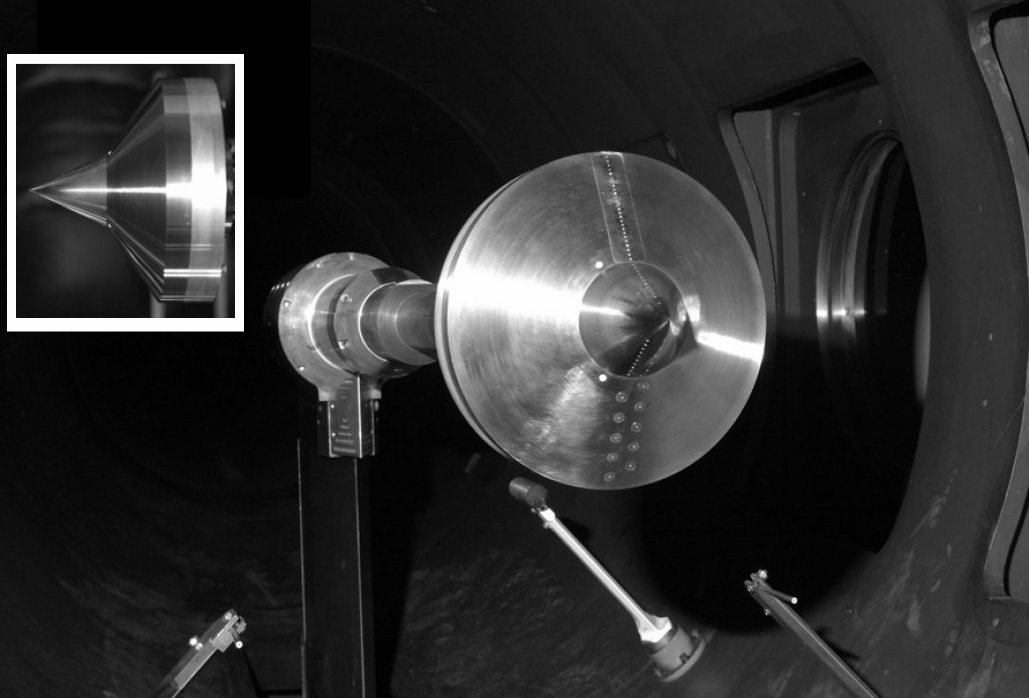
\includegraphics[width=\textwidth]{figures/aedc_double_cone/double_cone_HVWT9}
  \end{columns}
}

\frame
{
  \frametitle{\scriptsize Observations}
  \footnotesize
  \begin{itemize}
    \item Four Reynolds numbers were tested in the nominally Mach~14 nozzle
    \item No appreciable vibrational nonequilibrium effects observed
    \item Highly unsteady flow observed for \emph{all} Reynolds numbers tested
    \item For a uniform freestream, CFD predicts steady flow for the two lowest Reynolds numbers
  \end{itemize}

  \scriptsize
  \begin{center}
    \begin{tabular}{|l||ccccl|}\hline
      Run             & 2890 & 2891  & 2893  & 2894  & \\ \hline\hline
      &      &       &       &       & \\
      M$_\infty$      & 13.6 & 13.17 & 12.73 & 12.63 & \\
      &      &       &       &       & \\
      Re$_{\text{D}}$ & $1.12\times 10^{6}$ &  $4.11\times 10^{5}$ & $8.44\times 10^{4}$ & $5.86\times 10^{4}$ & \\
      &      &       &       &       & \\
      $\rho_\infty$      & 7.81$\times 10^{-3}$     & 2.96$\times 10^{-3}$     & 5.90$\times 10^{-4}$       & 3.98$\times 10^{-4}$     &   $\unitfrac{kg}{m^3}$ \\
      U$_\infty$      & 2006.6 & 1949.8 &  1763.5      & 1682.6     &   \unitfrac{m}{sec} \\
      T$_\infty$      & 52.3 & 52.7 & 46.1   & 42.7 & \unit{K} \\ \hline
    \end{tabular}
  \end{center}
}

\frame
{
  \frametitle{\scriptsize Steady states, runs 2893 and 2894}
  \begin{center}
    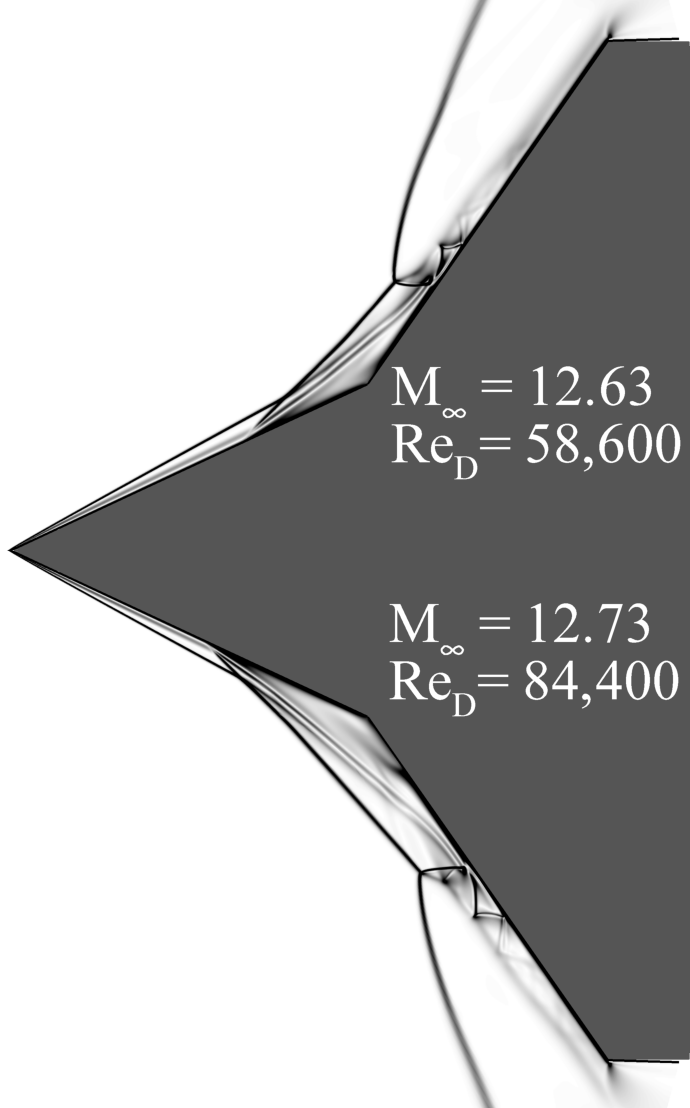
\includegraphics[height=.85\textheight]{figures/2893_2894_composite_schlieren}
    \hspace{2em}
    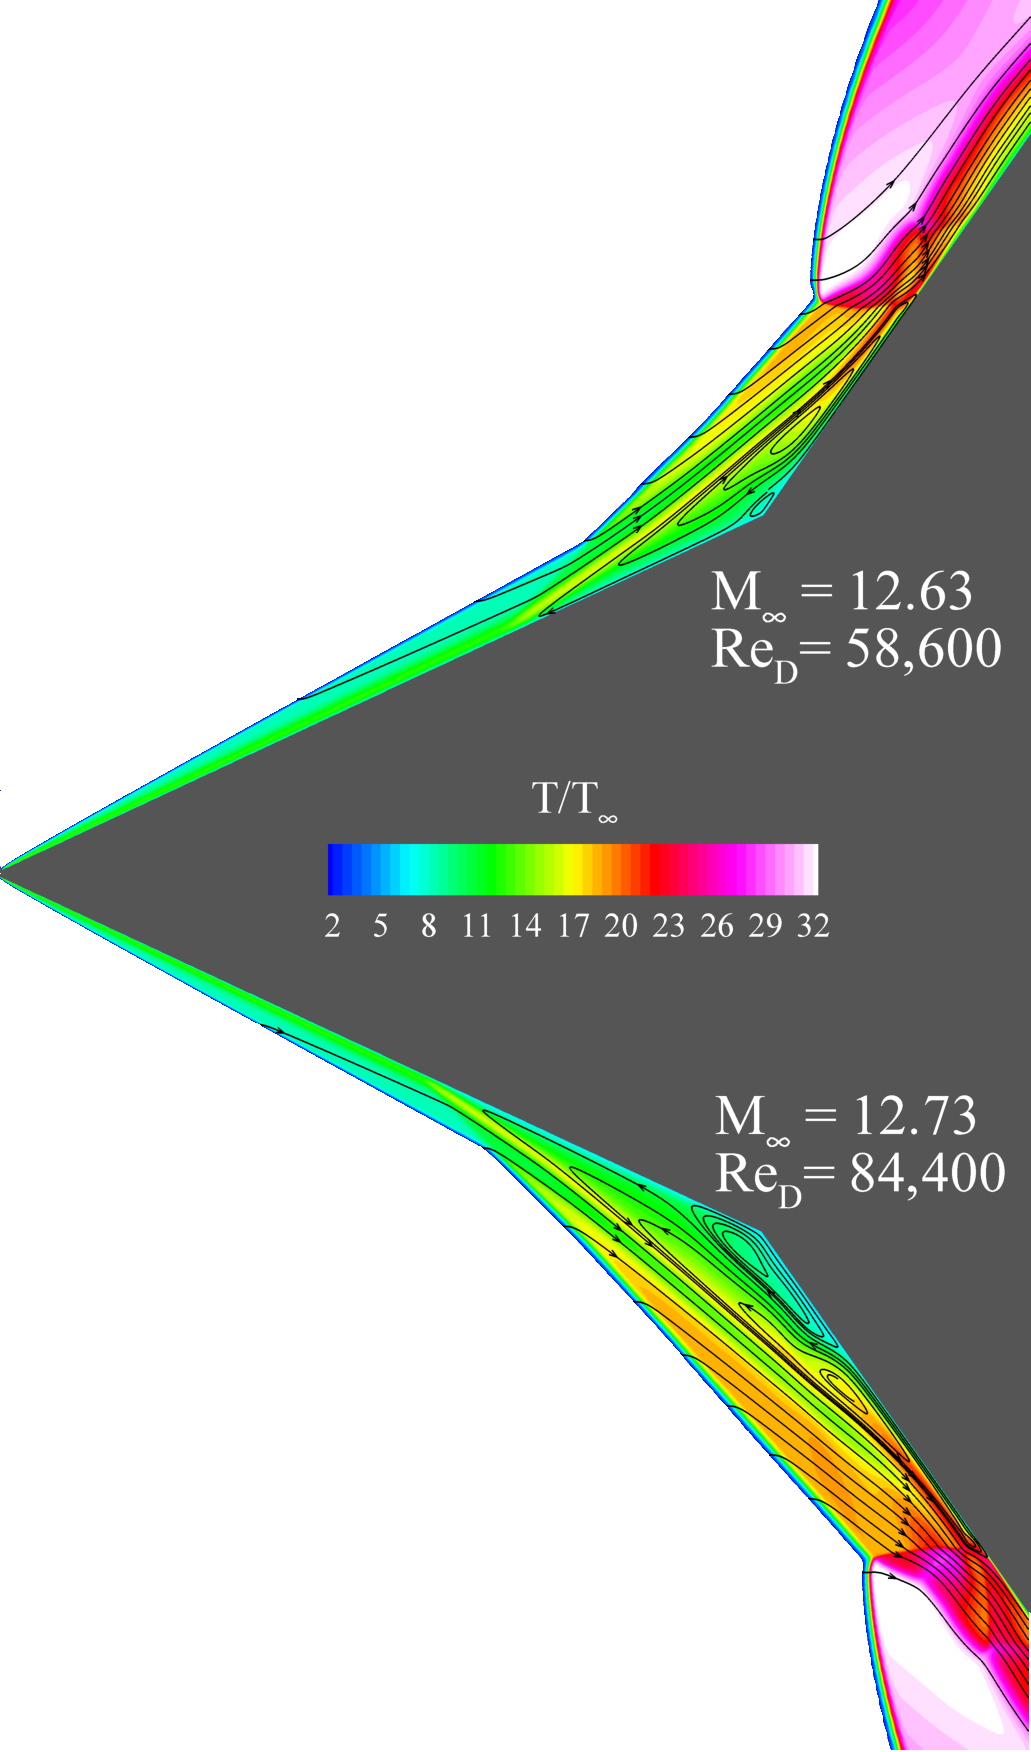
\includegraphics[height=.85\textheight]{figures/2893_2894_composite_streamlines}
  \end{center}
}

\frame
{
  \frametitle{\scriptsize Time Convergence, run 2894}
  \centerline{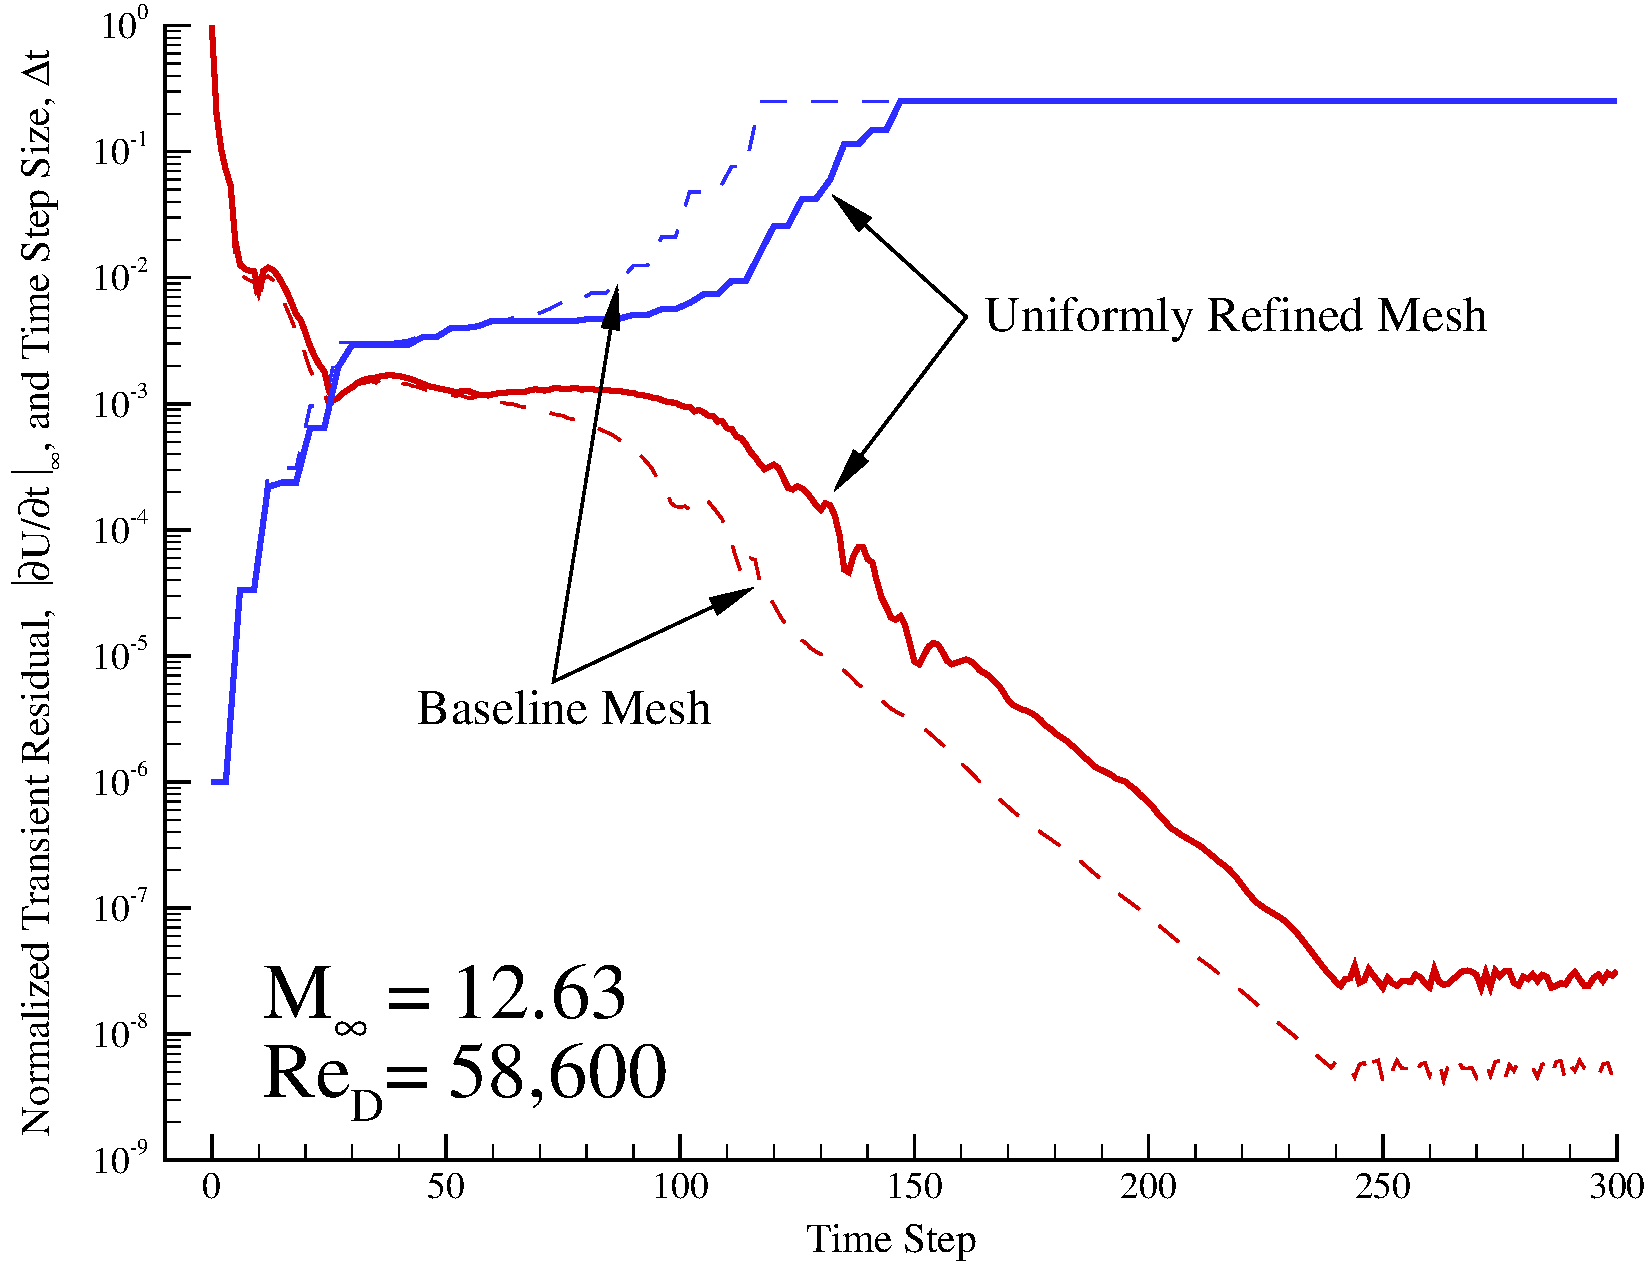
\includegraphics[height=.85\textheight]{figures/aedc_double_cone/2894/resid_history}}
}

\frame
{
  \frametitle{\scriptsize High speed schlieren, run 2890}
  \centerline{\includemovie[autoplay,loop,text={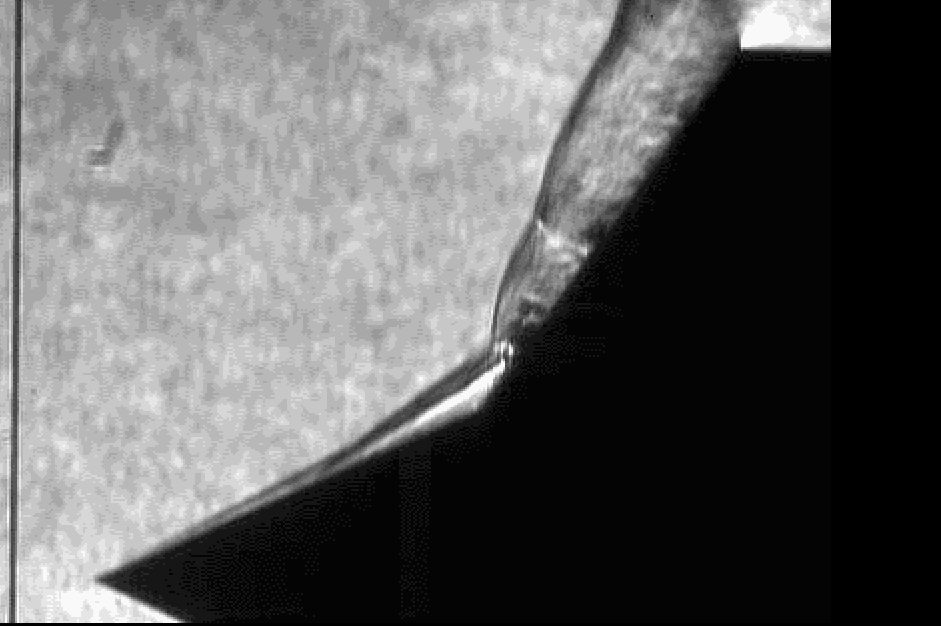
\includegraphics[height=.78\textheight]{figures/run2890}}]{.925\textwidth}{.78\textheight}{movies/run2890.avi}}  
}

\frame
{
  \frametitle{\scriptsize Computed schlieren, run 2890}
  \centerline{\includemovie[autoplay,loop,text={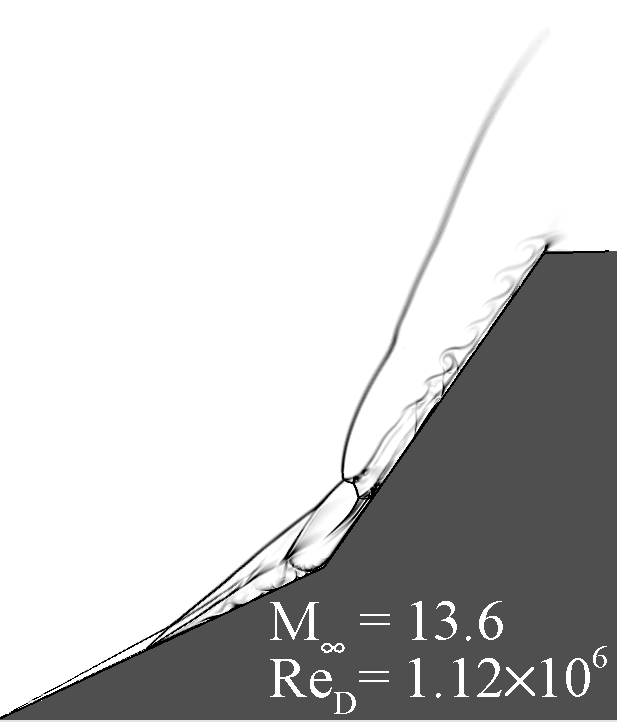
\includegraphics[height=.8\textheight]{figures/run2890_computed}}]{.55\textwidth}{.8\textheight}{movies/Schlieren_run2890.avi}}
}

\frame
{
  \frametitle{\scriptsize Possible Mechanism for Observed Unsteadiness}
  \begin{itemize}
    \item For a uniform inflow, CFD converges to a steady--state for the two lowest Reynolds numbers tested
    \item This is in contrast to the experimental results
    \item My conjecture is that freestream noise drives the unsteady behavior at these low Reynolds number
    \item Remaining analysis is focused on testing this theory
  \end{itemize}
}

\frame
{
  \frametitle{\scriptsize Noise Characterization~\cite{mcnalley_AEDC_noise}}
  \begin{center}
    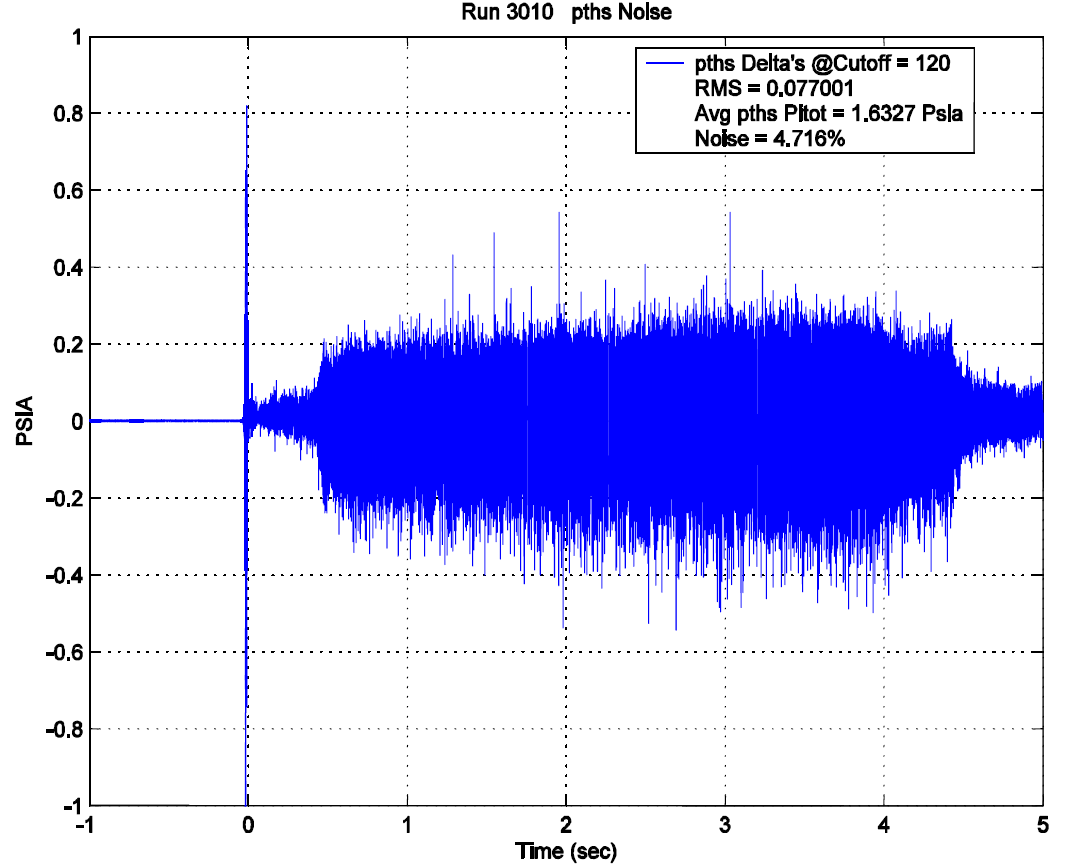
\includegraphics[width=.48\textwidth]{figures/aedc_noise/fluct}
    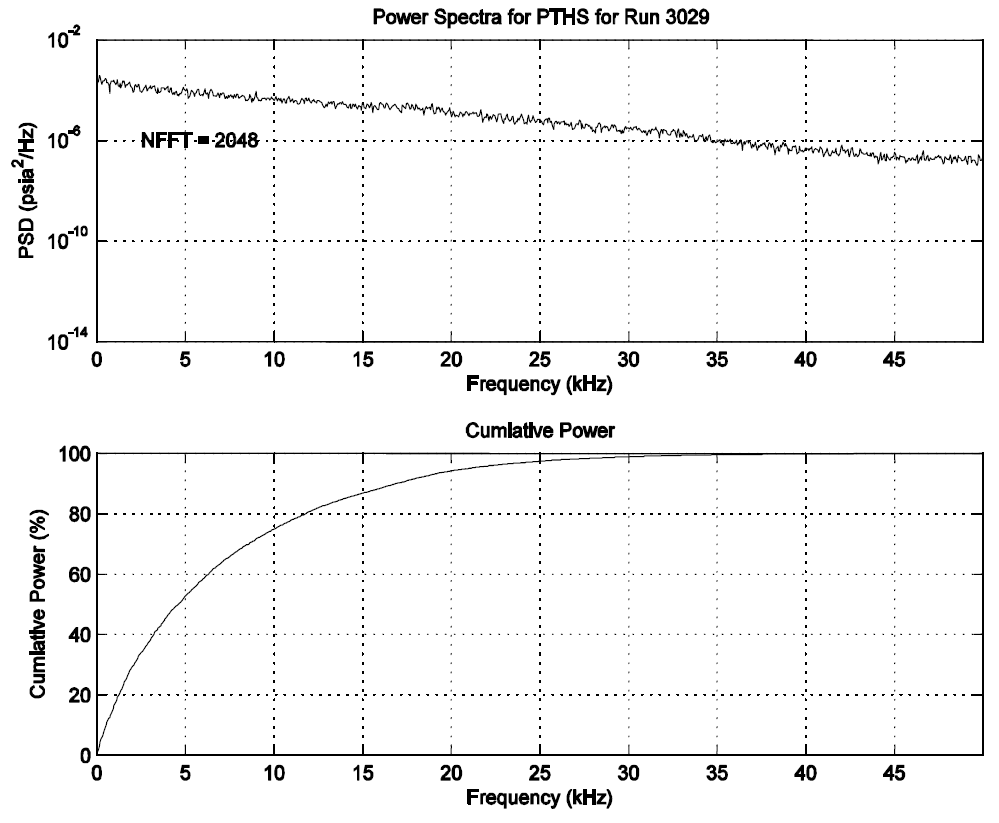
\includegraphics[width=.48\textwidth]{figures/aedc_noise/spectra}
  \end{center}
}

\frame
{
  \frametitle{\scriptsize Noise Characterization~\cite{mcnalley_AEDC_noise}}
  \vspace{-1em}
  \begin{center}
    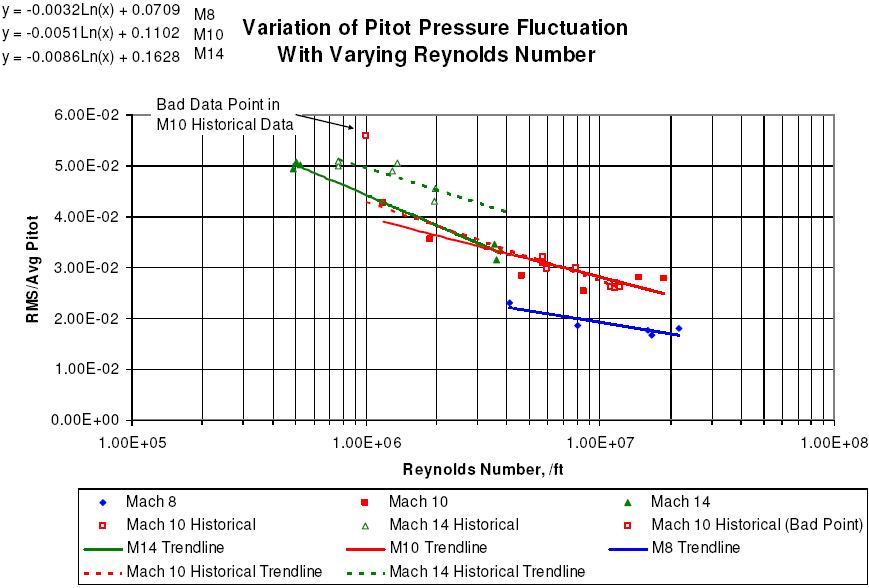
\includegraphics[height=.8\textheight]{figures/aedc_noise/noise}
  \end{center}
}

\frame
{
  \frametitle{\scriptsize Results -- Flowfield}
  \centerline{\includemovie[autoplay,loop,text={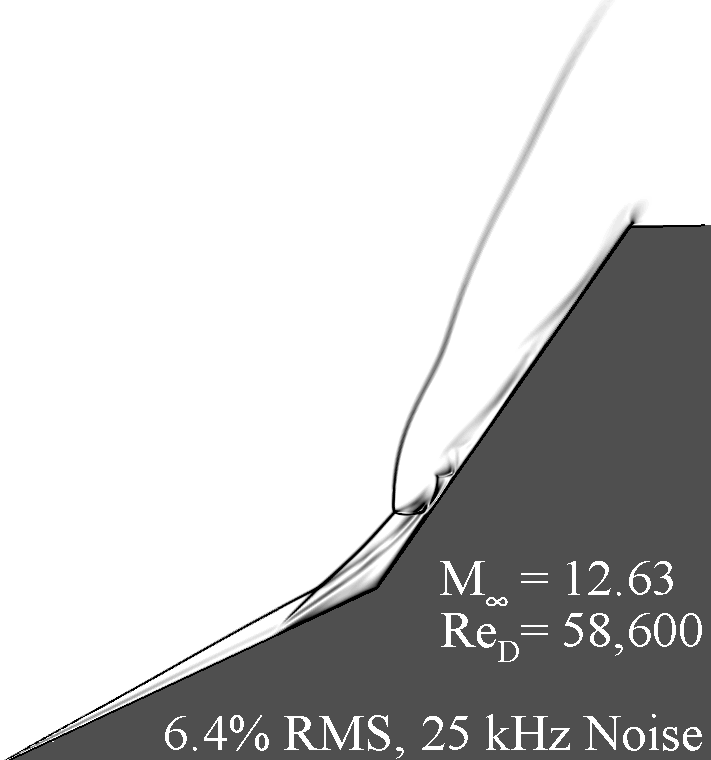
\includegraphics[height=.8\textheight]{figures/Schlieren_run2864}}]{.6\textwidth}{.8\textheight}{movies/Schlieren_run2864.avi}}
}

\frame
{
  \frametitle{\scriptsize Results -- Surface Pressure}
  \centerline{\includemovie[autoplay,loop,text={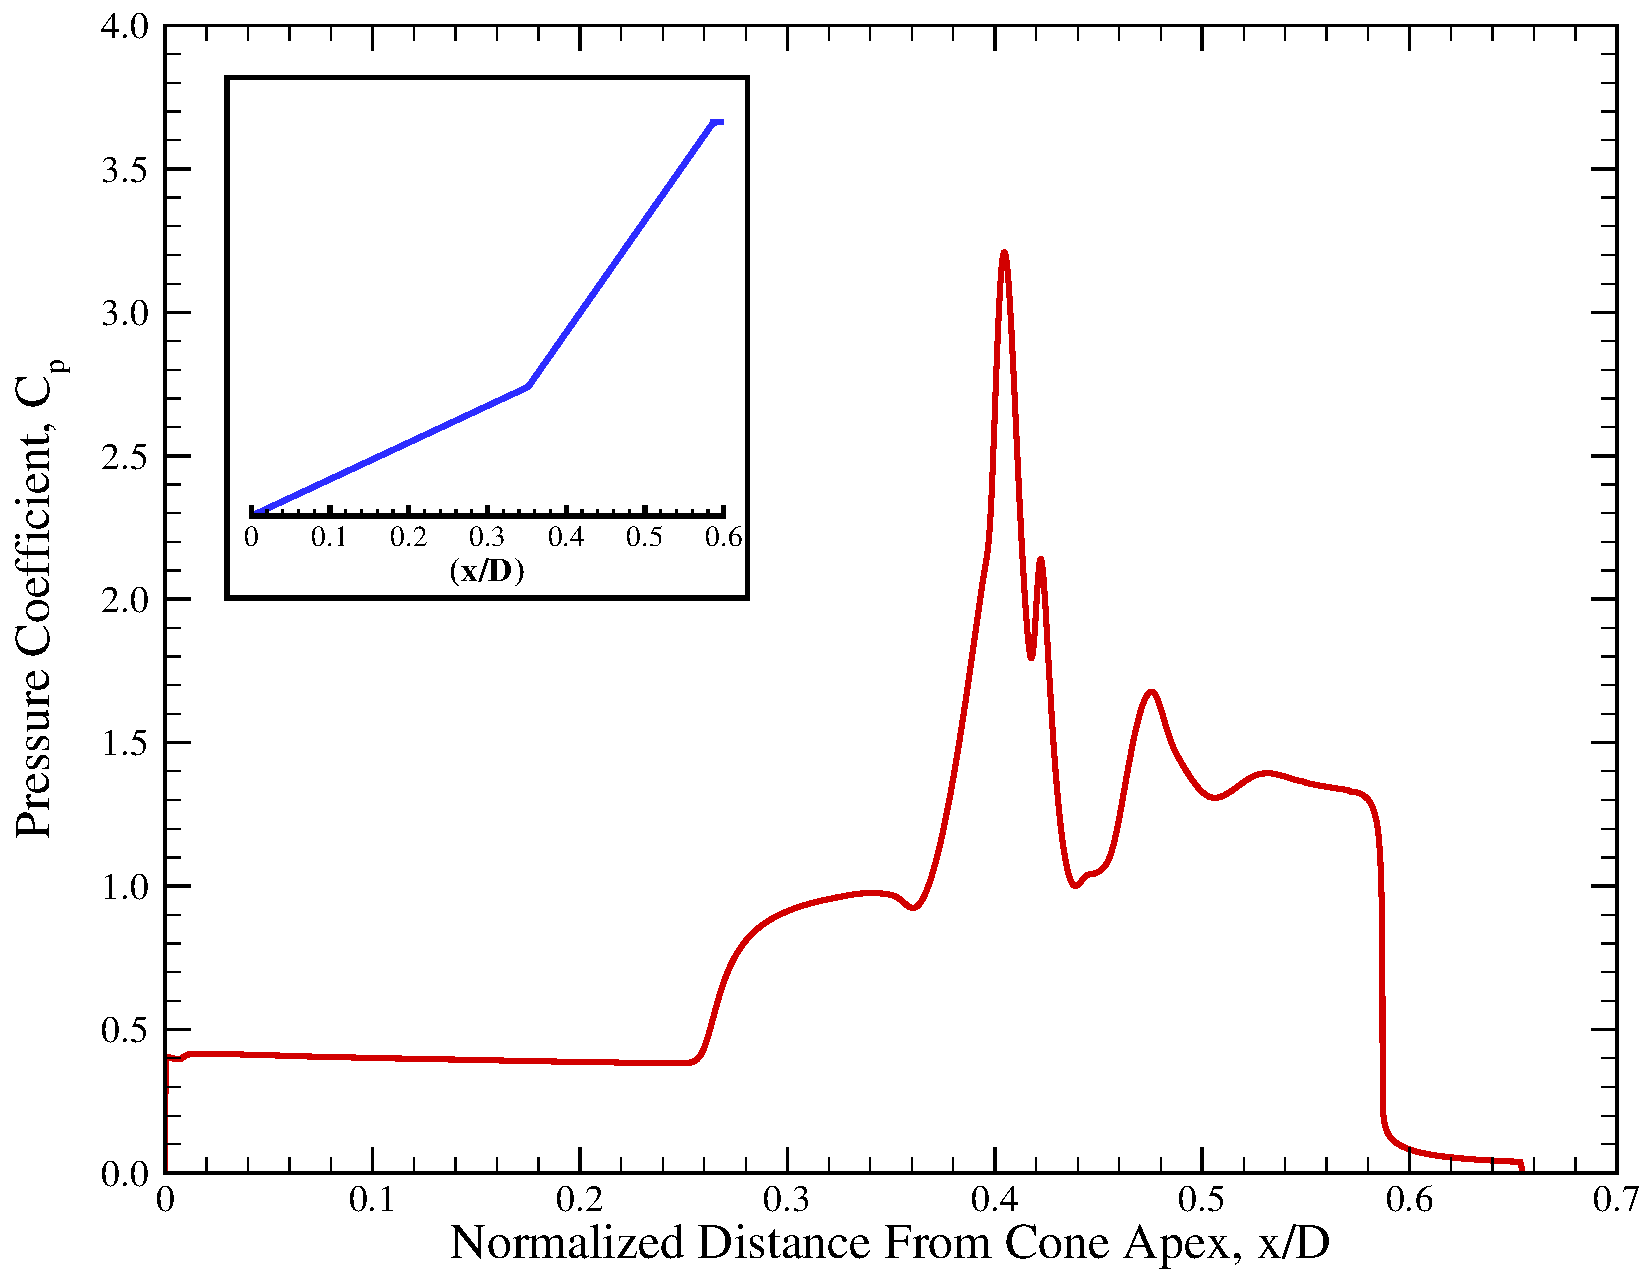
\includegraphics[height=.8\textheight]{figures/Cp_run2864}}]{.825\textwidth}{.8\textheight}{movies/Cp_run2864.avi}}
}

\frame
{
\frametitle{\scriptsize \unit[25]{kHz}, 6\% RMS Pitot Pressure Fluctuation}
\begin{center}
  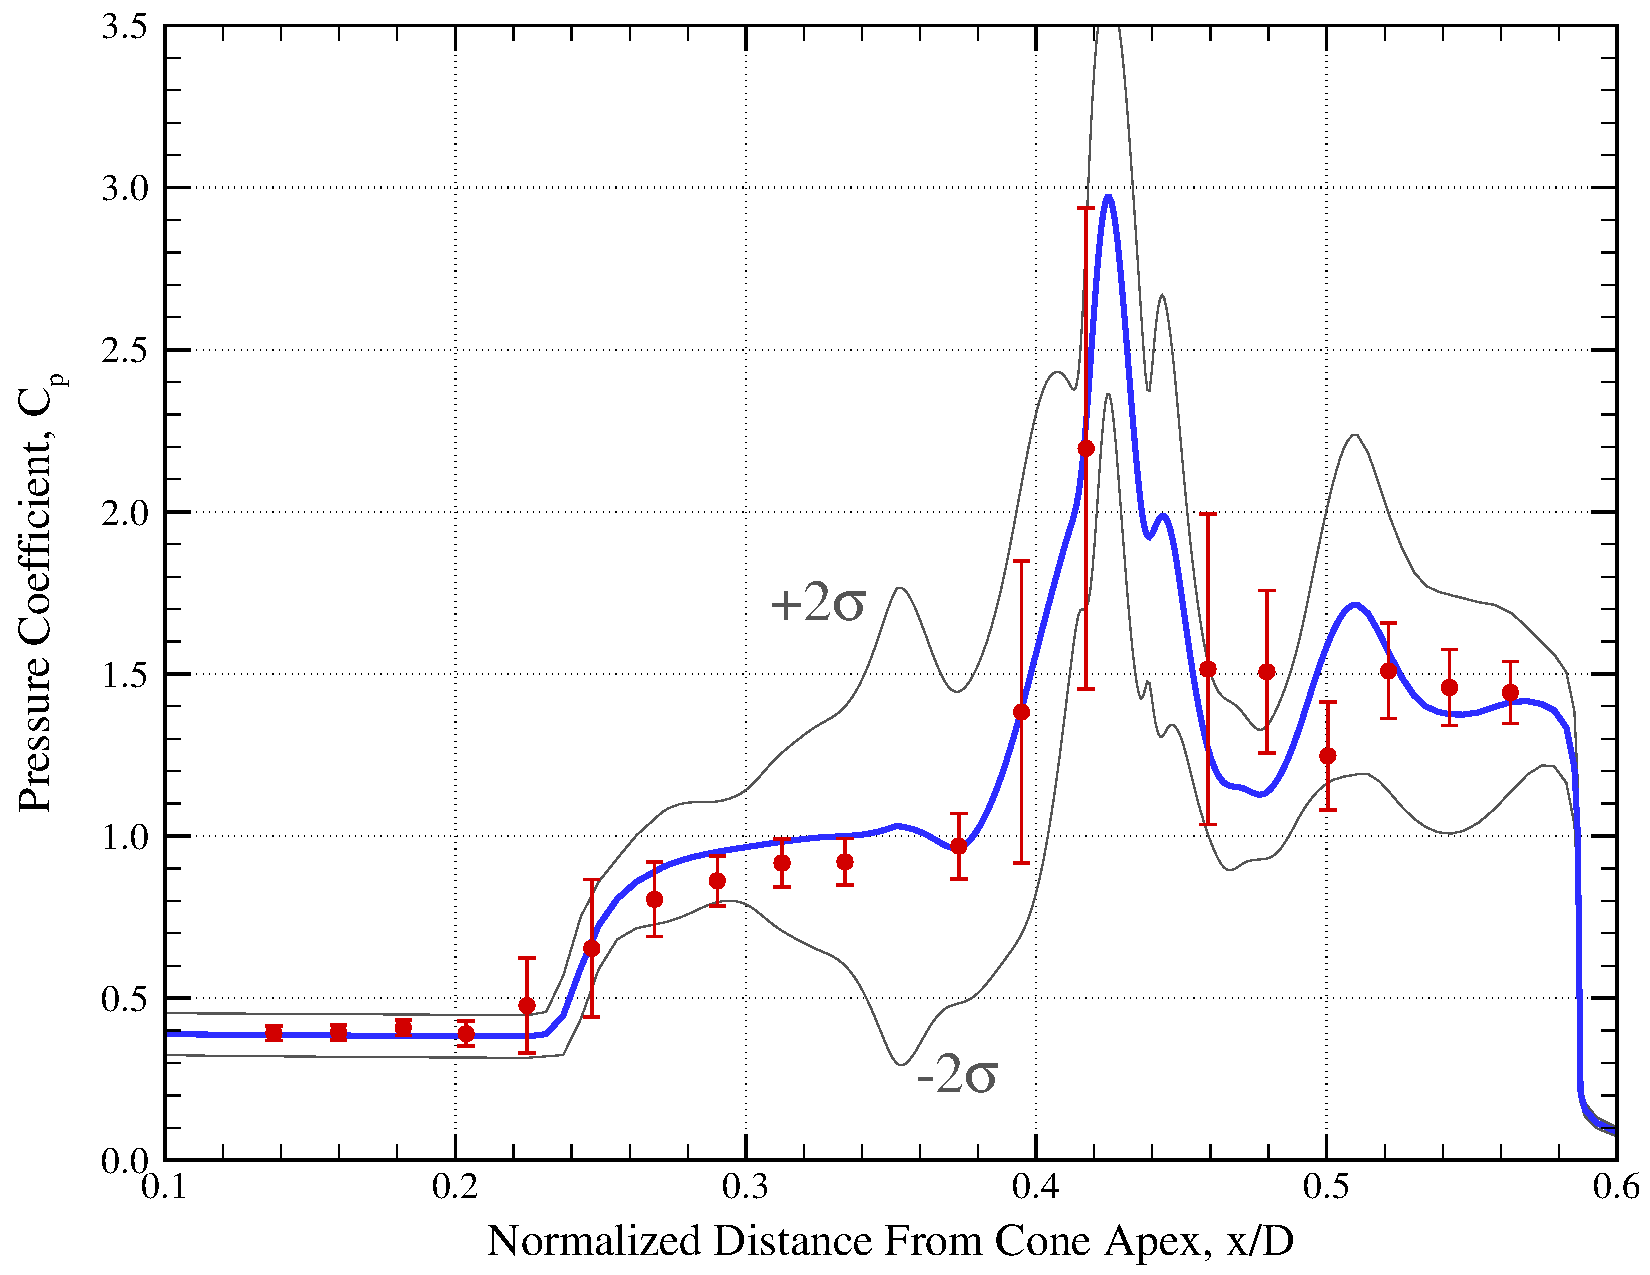
\includegraphics[width=.48\textwidth]{figures/aedc_double_cone/2894/Cp_25kHz_6percent}\hspace{.5em}
  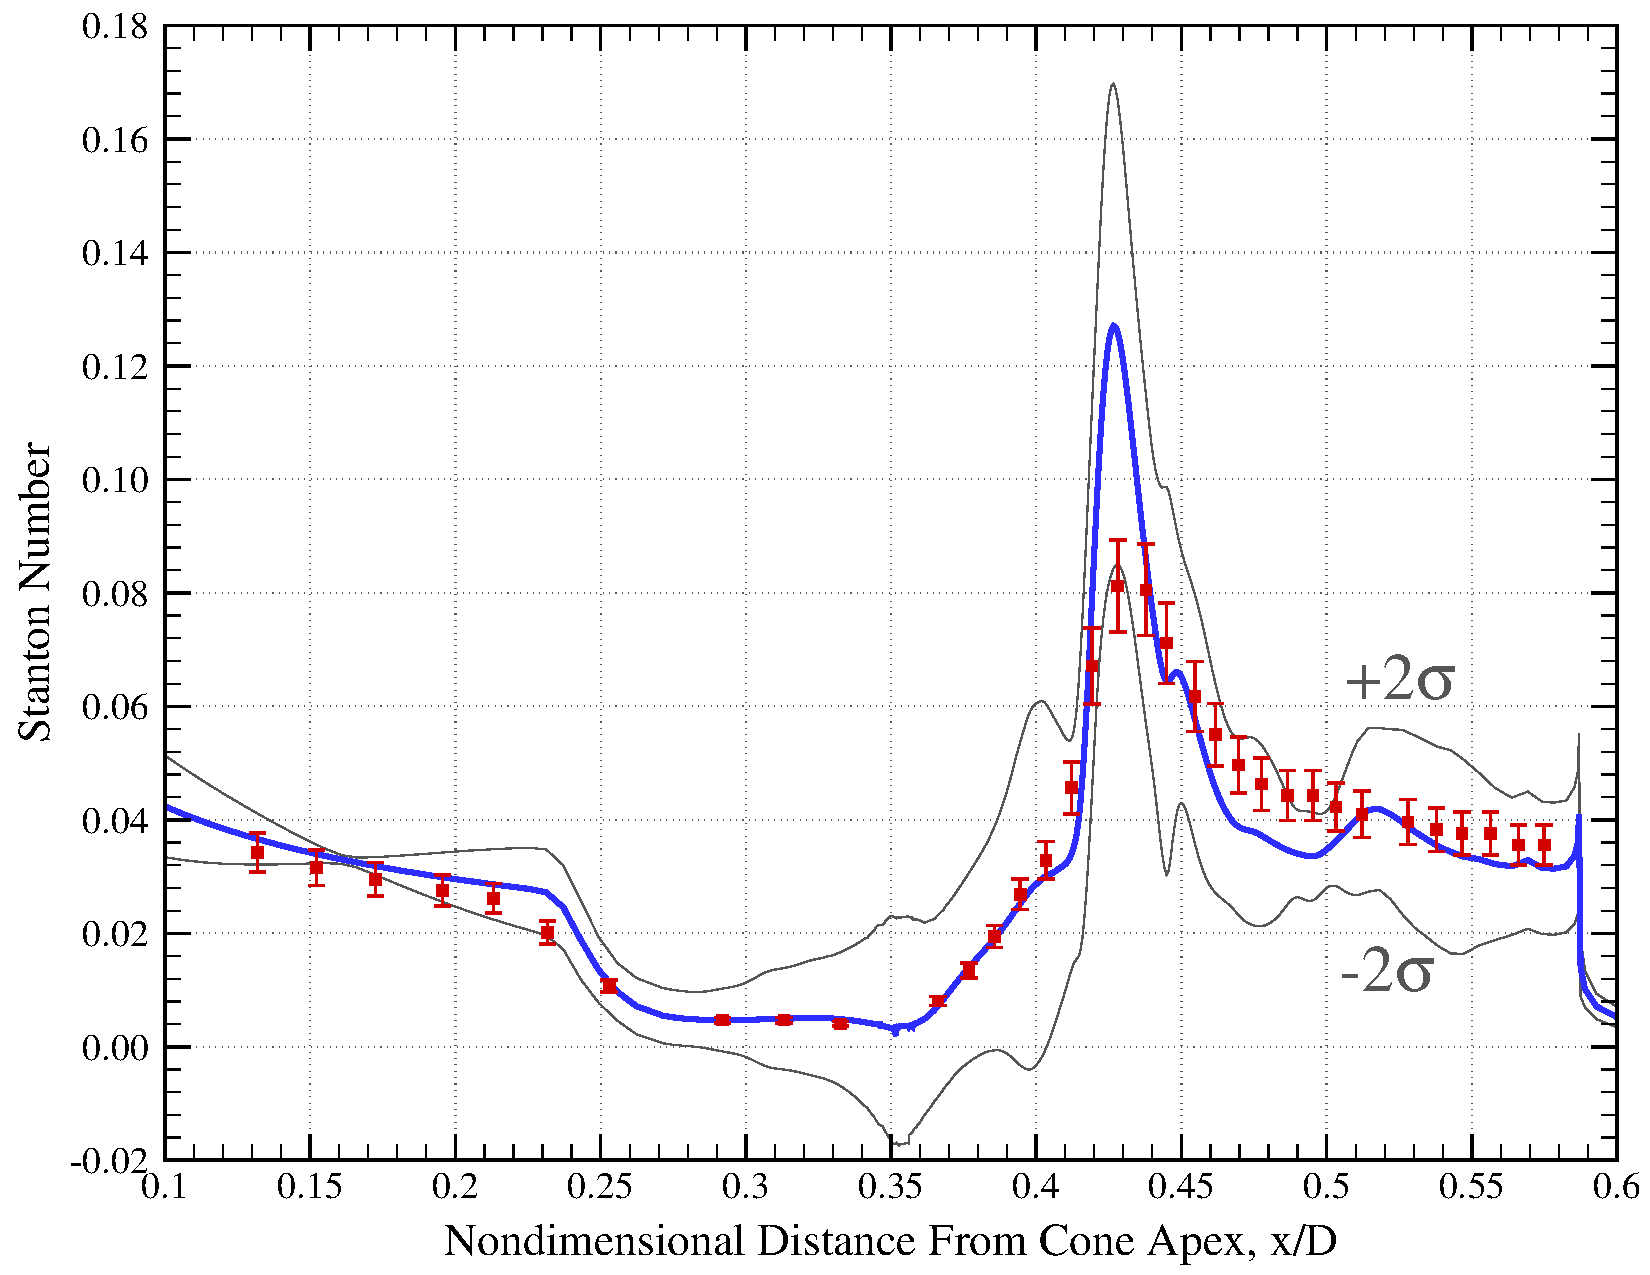
\includegraphics[width=.48\textwidth]{figures/aedc_double_cone/2894/St_25kHz_6percent}
\end{center}
}

\frame
{
\frametitle{\scriptsize Frequency Influence}
\begin{center}
  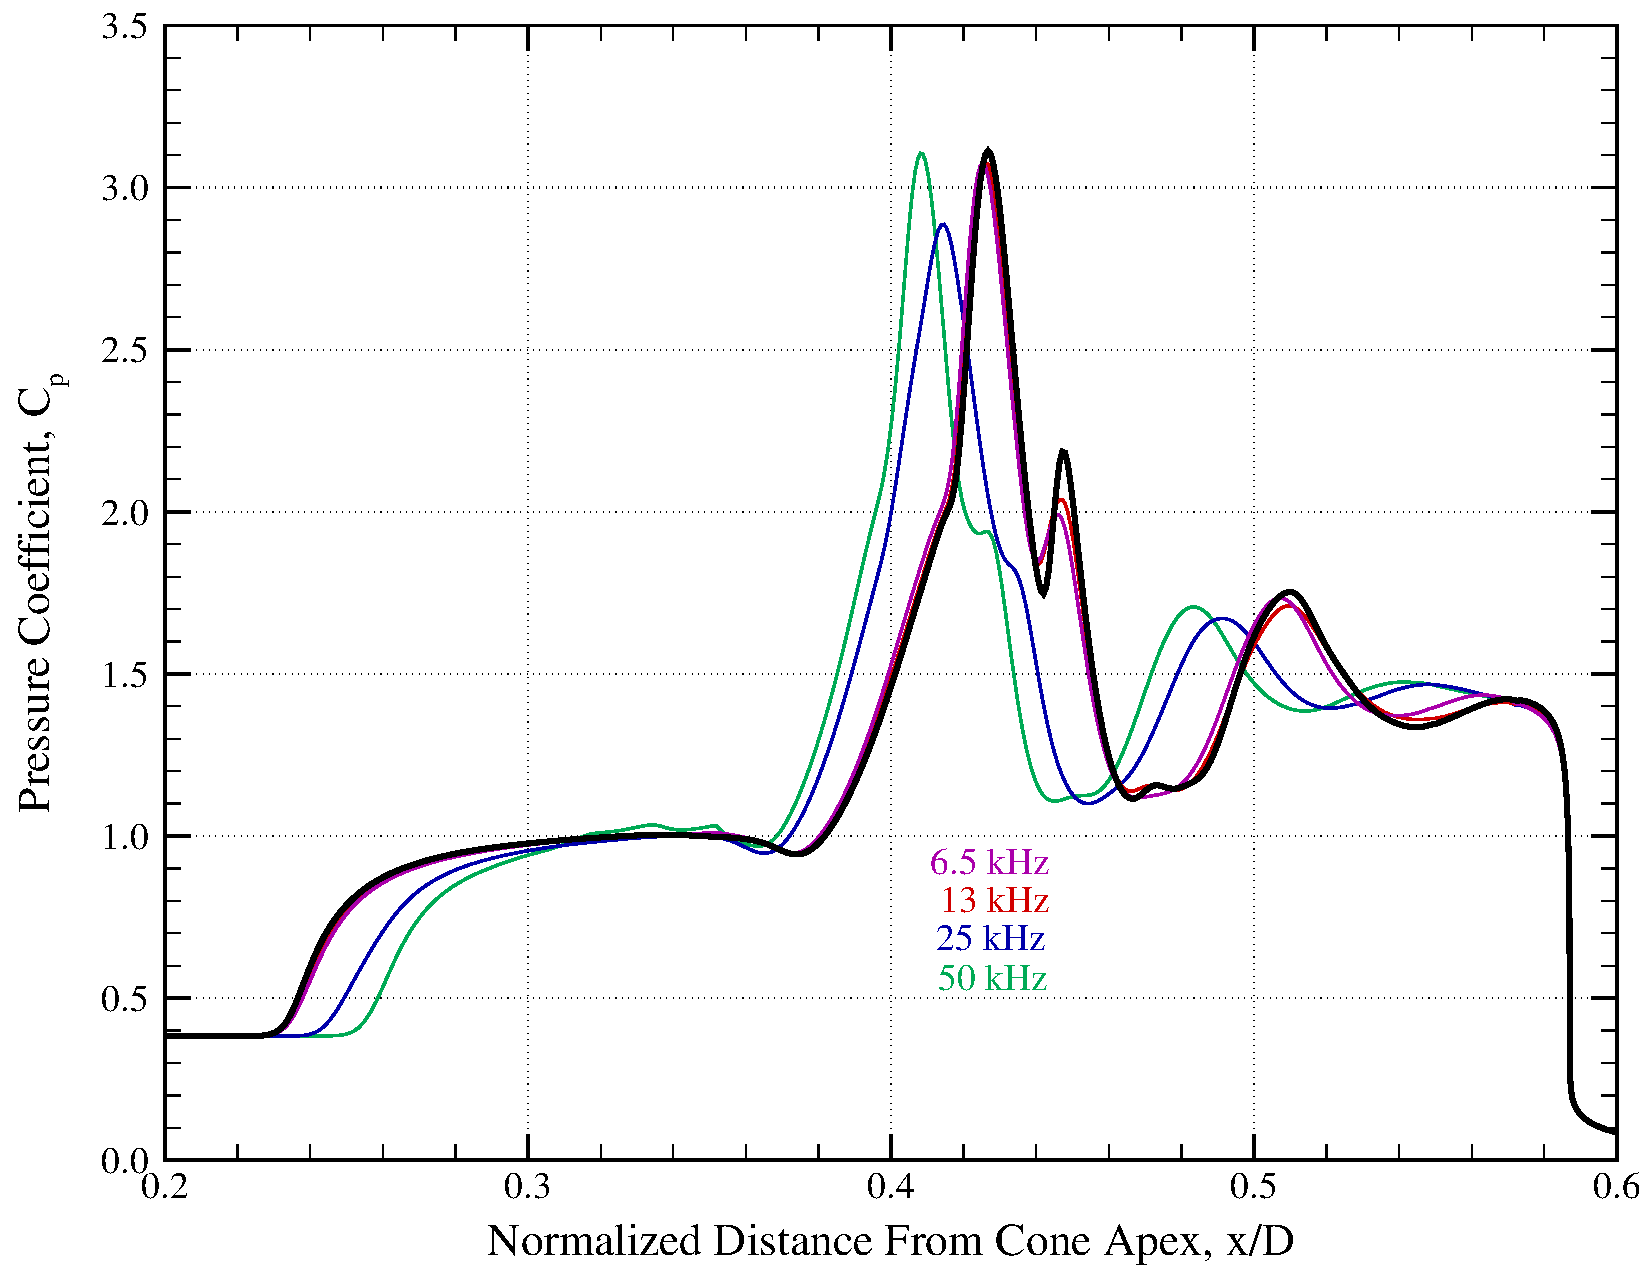
\includegraphics[height=.85\textheight]{figures/aedc_double_cone/2894/Cp_freq_comp}
\end{center}
}

\section*{Potential Collaboration}
\frame
{
  \frametitle{\scriptsize Potential Collaboration}
  \begin{itemize}
    \item Three-way comparisons between finite volume, SUPG finite element, and discontinuous Galerkin finite element methods for~\eqref{eq:pde_comp_mass}--\eqref{eq:pde_comp_energy} for problems of interest in aerothermodynamic design:
      \begin{itemize}
	\item Viscous/inviscid interactions
	\item Shock/boundary layer interaction
	\item Shock/shock interaction
      \end{itemize}
      \item Comparison of shock-capturing operator used here and novel developments by MIT ACDL faculty/students
      \item Rigorous evaluation of unstructured mesh quality and its influence in aerothermodynamic applications
  \end{itemize}
}

\section{Bibliography}
\setbeamertemplate{bibliography item}{}
\begin{frame}[allowframebreaks]{}
  \bibliographystyle{unsrt}
  \vspace{-1em}
  \tiny
  \bibliography{slides}
  \normalsize
\end{frame}

%% \frame
%% {
%%   \frametitle{\tiny Linear vs. Nonlinear Problems}
%%   \begin{columns}[t]
%%     \column{.5\textwidth}
%%     \begin{block}{Linear}
%%       \begin{itemize}
%%       \item Existence/Uniqueness usually proven
%%       \item Galerkin orthogonality
%% 	\begin{equation}
%% 	  \nonumber
%% 	  B(e,v^h) = 0 \;\;\;\forall v^h
%% 	\end{equation}
%%       \item Error representation
%% 	\begin{equation}
%% 	  \nonumber
%% 	  B(e,v) = L(v) - B(u^h,v) \;\forall v
%% 	  \end{equation}
%%       \end{itemize}
%%     \end{block}
%%     \pause
%%     \column{.5\textwidth}
%%     \begin{block}{Nonlinear}
%%       \begin{itemize}
%%       \item Existence/Uniqueness only under certain restrictions
%%       \item Galerkin orthogonality
%%        \begin{equation}
%% 	 \nonumber
%% 	 (\mathscr{R}(u), v) = 0 \;\;\;\forall v
%%        \end{equation}
%%        \item Error representation
%% 	 \begin{equation}
%% 	   \nonumber
%% 	   (\mathscr{R}(u-u^h), v) = ?
%% 	 \end{equation}
%%       \end{itemize}
%%     \end{block}

%%     \end{columns}
%% }


%% \section{Explicit A Posteriori Error Estimators}
%% \subsection{Kelly et. al Error Estimator}
%% \frame
%%     {
%%       \frametitle{\tiny A Model Problem}

%%       \begin{eqnarray}
%% 	-\Delta u &=& f \;\;\; \in \Omega \\
%% 	u&=&g \;\;\; \in \partial \Omega
%%       \end{eqnarray}

%%       \uncover<2->
%% 	  {
%%       \begin{block}{Regularity}
%% 	Under certain assumptions on $\Omega$ and the data,
%% 	the solution $u\in C^2(\Omega)$ exists and is unique.
%%       \end{block}
%%       }
%%     }

%% \frame
%%     {
%%       \frametitle{\tiny The variational form}
      
%%       %\begin{itemize}
%% 	\only<1>
%% 	{
%% 	  \begin{equation}
%% 	    \nonumber
%% 	    \int_{\Omega} \nabla u \cdot \nabla v \;dx =
%% 	    \int_{\Omega} fv \; dx \;\;\;\forall v \in V
%% 	  \end{equation}
%% 	  }
	
%% 	\only<2>
%% 	{
%% 	  \begin{equation}
%% 	    \nonumber
%% 	    \int_{\Omega^{\alert{h}}} \nabla u^{\alert{h}} \cdot \nabla v^{\alert{h}} \;dx =
%% 	    \int_{\Omega^{\alert{h}}} fv^{\alert{h}} \; dx \;\;\;\forall v^{\alert{h}} \in V^{\alert{h}}
%% 	  \end{equation}
%% 	}
%%       %\end{itemize}
%%     }

\end{document}


% LocalWords:  AEDC LaRC forebody DPLR Lomax blayer Freestream cccccc eq pde ij
% LocalWords:  upwinding SUPG Galerkin Petrov shockwaves discretization udot un
% LocalWords:  discretizations semidiscrete discretized unm euler ccc DOF GMRES
% LocalWords:  ILU linearization de rospatiales ONERA flowfield freestream CFD
% LocalWords:  autoplay CUBRC nonequilibrium rrrrl schlieren Navier calorically
% LocalWords:  Aerothermodynamics aerothermodynamics LeBeau Tezduyar al Krylov
% LocalWords:  Edney's ccccl CFL Multiscale ACDL aerothermodynamic superorbital
